\documentclass[dissertation, copyright, final, gsmodern]{uothesis_3}
\setcounter{tocdepth}{2}
\setcounter{secnumdepth}{4}
\usepackage[linktocpage]{hyperref}
\usepackage[USenglish]{babel}
\usepackage{todonotes}
\usepackage{subfig}
\usepackage{enumitem}
\usepackage{caption}
\usepackage{notoccite}
\usepackage{siunitx}
 %\sisetup{separate-uncertainty,table-format=6.3(6)}
\usepackage{booktabs}
\usepackage{slashed}
\usepackage{amsmath}
\usepackage{amssymb}
\usepackage{feynmp}
\usepackage[utf8]{inputenc}
\usepackage{pdflscape}
\usepackage{url}
\usepackage{lineno}
%\linenumbers %%%%%%%%%%%%%%LINE NUMBERS - Only works once, need to compile without and then uncomment to work
\usepackage{multicol}
%\usepackage{appendix}
%\usepackage{itemize}
\linenumbers
\usepackage{longtable}
\usepackage{pdflscape}
\usepackage{xfrac}
\usepackage{hhline}
\usepackage{tabularx}
\setcounter{tocdepth}{3}% Include \subsubsection in ToC
%\usepackage{hyperref} %If you get an error due to hyperref package, delete your old INT.aux file then recompile.
%\usepackage[nonatbib]
\usepackage[style=numeric-comp,backend=biber,sorting=none]{biblatex}
\addbibresource{main.bib}
\pdfstringdefDisableCommands{\let\uppercase\relax}

\justifiedtrue

% hold floats in their (sub)section
\usepackage{placeins}
\let\Oldsection\section
\renewcommand{\section}{\FloatBarrier\Oldsection}
\let\Oldsubsection\subsection
\renewcommand{\subsection}{\FloatBarrier\Oldsubsection}
\let\Oldsubsubsection\subsubsection
\renewcommand{\subsubsection}{\FloatBarrier\Oldsubsubsection}

\renewcommand{\labelitemi}{$\bullet$}

\newcommand*{\ifb}{\mbox{fb$^{-1}$}}
\newcommand*{\ipb}{\mbox{pb$^{-1}$}}
\newcommand*{\pt}{\ensuremath{p_{\text{T}}}\xspace}
\newcommand*{\mjj}{\mbox{$m_{jj}$}}

%\setcounter{tocdepth}{0}
\begin{document}

\covertitle{Search for the Flavor-Changing Neutral Current in Top Pair Events With an Associated Photon Using 13 TeV Proton-Proton Collision Data Collected With the ATLAS Detector}
\abstracttitle{Search for the Flavor-Changing Neutral Current in Top Pair Events With an Associated Photon Using 13 TeV Proton-Proton Collision Data Collected With the ATLAS Detector}
\author{Jason Tyler Barkeloo}
\department{Department of Physics}%Make sure to capitalize physics
\narrowdepartment{Department of Physics}
\degreetype{Doctor of Philosophy}
\degreemonth{March}%The month you earn the degree, different than the month you defend - CHANGE CHECK
\degreeyear{2019}
\advisor{James Brau}
\chair{David Strom}
\committee{Spencer Chang & Core Member \\
Dev Sinha & Institutional Representative \\	}
\graddean{Janet Woodruff-Borden}%CHANGE CHECK THIS
\abstract{
Abstract for FCNC here.

%Need to end with this statement if you're working from papers published or soon to be published.
This dissertation includes previously published and unpublished co-authored material.
}
\author{Benjamin William Allen}
\school{University of Oregon, Eugene}%Graduate school
\school{University of California, Irvine}%Undergraduate school

\degree{Doctor of Philosophy, Physics, 2018, University of Oregon, Eugene}%Change year
\degree{Bachelor of Science, Physics, 2010, Univeristy of California, Irvine}%Undergraduate degree

%%There is a known issue if you do not fill in the interests section.  If you want to skip this section, comment out line#526 of uothesis.cls file \cvitem{GRANTS, AWARDS AND HONORS}{\@awards}
%\interests{}%Your interests. French movies, long walks on the beach, baking tarts...

\position{\textbf{University of Oregon}, Graduate Research Assistant, ATLAS Experiment, June 2014-Present}
\position{\textbf{University of Oregon}, Graduate Teaching Assistant, September 2012-June 2014}%Your job while at UO, probably graduate research assistant.


\award{Fall Qualifying Exam Award -- October 2014}%If you didn't get any awards you'll have to comment out things in the uothesis. I dug up something from my undergraduate
\publication{ATLAS Collaboration, "Search for new phenomena in dijet mass and angular distributions from pp collisions at with the ATLAS detector", Physics Letters B, Volume 754, 10 March 2016, Pages 302-322}
\publication{ATLAS Collaboration, "Search for new phenomena in dijet events collected in 2015 and 2016 pp collisions with the ATLAS detector at $\sqrt{s}$ = 13 TeV", ATLAS-CONF-2016-069, 2016}
%Fill this out with your publications.



%\acknowledge{%Thanks go here.

To my fellow undergrads, grads, and post-docs at Oregon: Walter, Kate, Aparajita, Chris, Liza, Max, Peter, Ian, Jason, John, Johan, Elliot, Bri, Amanda, Aaron, and many more. Thank you all for for encouragement, help, questions, and camraderie.

My dijet partners-in-crime: James, Marco, Matteo, Karishma, Kate, Meghan, Caterina.  Thank you for showing me the ropes and suffering along side me through each pressing deadline.

For Sarah, who kicked my butt into going to grad school, who thought we'd never end up in Oregon, much less Europe.  Thank you for being my support and my travel buddy, and forcing me to go outside.

For January, who refused to nap and let this be written.

}

  %%acknowledgements page optional
\maketitle

\newpage
\section{Introduction}
\label{sec:intro}
%Deep thoughts go here.

The Standard Model of particle physics has proven itself an exceptional and resilient theory since the combination of the electromagnetic and weak interactions in 1961\cite{SM1Glashow}.  Further theoretical work combined the Higgs Mechanism\cite{Higgs1,Higgs2} with the electroweak theory\cite{SM2Weinberg, SM3Salam}.  The resiliency of this theoretical model has been tested to further degrees of accuracy over the decades with one of my most recent portions being the experimental confirmation of the Higgs Boson in 2012\cite{Higgs3,Higgs4} using the Large Hadron Collider (LHC).  Further precision measurements are ongoing at various experiments at the LHC, including the ATLAS experiment.

However, the Standard Model is known to have flaws and disagreements with nature.  For example, the Standard Model predicts massless neutrinos which is in conflict with experimental observation of neutrino flavor oscillation and doesn't provide an explanation for dark matter particles or their interactions with currently known particles.  While these large gaps in the Standard Model are well known every precision measurement made has yet to give any significant new hints toward physics beyond the Standard Model.  One new pathway to look for these hints at the LHC is through top quark decays.

\subsection{The Standard Model Top Quark}
The top quark was first observed at Fermilab's Tevatron in 1995\cite{TopObs} but the increase in energy and amount of data at the LHC has produced orders of magnitude more top quarks than previously seen opening up a pathway to precision measurements of the properties of the top quark.  The top quark is the heaviest fundamental particle with a mass of 172.51 $\pm$ 0.27 (stat) $\pm$ 0.42 (syst)\cite{TopMass2017}.  This large mass also means that top top quark lifetime is very short (5 * 10$^{-25}$ s) and decays before it can hadronize.  This allows us to probe its' branching ratios and decay modes directly.  The Standard Model predicts that the top quark decays through the charged current mode nearly 100\% of the time; t$\rightarrow$ qW (q = b,s,d)\cite{PDG2018}.   The Standard Model also predicts a rare branching ratio of the top quark through a flavor changing neutral current (FCNC) process, to a neutral boson (photon, Z boson, Higgs Boson, or gluon) and up type quark with a branching ratio on the order of 10$^{-14}$.

\subsection{Searching for FCNC Top Quark Decays}
Precision measurements are an important litmus test for the Standard Model.  Predicted branching ratios for FCNC processes in top quark decays are far beyond the experimental reach of the LHC and any observation of these decay modes would be a sure sign of new physics.  Branching ratios are an important measurement due to a litany of theories for new physics beyond the Standard Model (BSM).  These BSM theories predict enhancements in the top sector by many orders of magnitude such as Minimal Supersymmetric models\cite{MSSM}, R-parity-violating Supersymmetic models\cite{RPVSUSY} and two Higgs doublet models\cite{2HDM} can all increase this branching ratio many orders of magnitude.  Even a null result to a search will set an upper limit on the branching ratio that can assist in ruling out future physical models based on their amount of large top sector enrichment.

This dissertation presents a search for top FCNCs using the entire Run 2 dataset at the LHC, containing combined 2015-2018 datasets taken by the ATLAS experiment totaling 139 fb$^{-1}$ of integrated luminosity taken at $\sqrt{s}$= 13 TeV.  The analysis presented looks for an excess of events coming from top quark pair produced events where one top quark decays to the most likely decay mode (a bottom quark and W boson) and the other to an up type quark (up or charm) and a photon. Section \ref{ch:Theory} a theoretical background will be presented for both the Standard Model with a closer view on the usual extensions to include the FCNC vertices.  Following this  Section \ref{ch:LHCDetector} will discuss the LHC and the ATLAS experiment used in the creation of the dataset used in the analysis.  In Section \ref{ch:Simulation} the special signal simulation requirements will be presented as well as the common background event simulation methodology.  The search strategy including the creation of signal, control and validation regions and the training of a neural network will be examined in Section \ref{ch:SearchStrategy}.  Section \ref{ch:Results} will discuss the results and the conclusions drawn from these results will be presented in Chapter \ref{ch:Conclusion}.

\chapter{Theory}
\label{ch:Theory}

In this chapter a theoretical background will be presented on the Standard Model of particle physics with special attention paid to the top quark's properties and decays.  This will include discussion of all of the fundamental particles and their interactions through the fundamental forces of nature: electromagnetism and the strong and weak nuclear forces.

%%%%%%%%%%%%%%%%%%%%%%%%%%%%%%%%%%%%%%%%%%%%%%%
%%%%%%%%%%%%%%%%%%%%%%%%%%%%%%%%%%%%%%%%%%%%%%%
\section{The Standard Model Particles}
\label{SMParticles}
The Standard Model of Particle Physics is the cornerstone of our understanding of the basic building blocks of nature and their interactions with one another.  Typical matter is made up of atoms consisting of electrons around an inner nucleus consisting of protons and neutrons.  These protons and neutrons are made up of a collection of up and down type quarks along with sea quarks and gluons.  Protons consist of two up type quarks and a down type quark while neutrons contain two down type quarks and a single up type quark.  

Within the Standard Model all matter (quarks and leptons) is made up of fermions (spin-$\frac{1}{2}$ particles).  In addition to the up and down type quarks and the electron the remaining fermions can be decribed as additional 'generations' that are similar, each consisting of two quarks and a lepton.  Every generation consists of quarks with electric charge $+\frac{2}{3}$ and $-\frac{1}{3}$ and a lepton with charge $-1$ along with an electrically neutral lepton called a neutrino.  All of these fermions are listed in Table \ref{tab:SM}.  

While we can observe the leptons in nature free quarks do not exist.  We can observe quarks only as part of a bound state called a hadron.  If a hadron consist of a quark-antiquark pair ($q\bar{q}$) it is called a meson.  Sets of three quarks or three antiquarks ($qqq$ or $\bar{q}\bar{q}\bar{q}$) are called baryons.  Protons and neutrons are baryonic matter.

In addition to the fermions the Standard Model contains gauge, or vector, bosons which are spin-1 particles that carry the fundamental forces of nature.  The electromagnetic foce is mediated by the massless, charge neutral photon ($\gamma$). The nuclear weak force is carried by two massive bosons: the electrically neutral Z boson and the charged ($\pm 1$) W boson.  These bosons together dictate electroweak interactions within the Standard Model.  The remaining force, the nuclear strong force, is carried through the gluon ($g$).  Gluons are massless and chargeless but carry color, an analog of electric charge in the electroweak interaction.  The last remaining piece of the Standard Model is the scalar (spin-0) Higgs boson.  This Higgs boson is a massive electrically neutral boson that is responsible for giving mass to the massive fundamental particles.  All of these bosons are also shown in Table \ref{tab:SM}.  

\begin{table}[h]
\begin{center}
\footnotesize
\begin{tabular}[h]{|c||c|c|c|c|}
\hline
 & Particle & Spin & Charge & Mass \\
\hline\hline
Quarks &&&&\\
\hline
u type &u& & &${2.4^{+0.6}_{-0.4} \text{ MeV}}$\\
 &c&${\frac{1}{2}}$&${\frac{2}{3}}$&${1.28\pm{0.03} \text{ GeV}}$\\
 &t& & &${173.1\pm{0.6} \text{ GeV}}$\\
\hline
d type & d& & & ${4.7^{+0.5}_{-0.4} \text{ MeV}}$\\
 & s & ${\frac{1}{2}}$ & ${-\frac{1}{3}}$ & ${96^{+8}_{-4} \text{ MeV}}$\\
 & b & & & ${4.18^{+0.04}_{-0.03} \text{ GeV}}$\\
\hline\hline
Leptons &&&&\\
\hline
e doublet & e & ${\frac{1}{2}}$ & -1 &${0.5109989461\pm{}0.000000003 \text{ MeV}}$\\
 & ${\nu_{e}}$ & & 0 & ${< 2 \text{ eV}}$\\
 \hline
${\mu}$ doublet & ${\mu}$ & ${\frac{1}{2}}$ & -1 &${105.6583745\pm{}0.0000024 \text{ MeV}}$\\
 & ${\nu_{\mu}}$ & & 0 & ${< 2 \text{ eV}}$\\
 \hline
${\tau}$ doublet & ${\tau}$ & ${\frac{1}{2}}$ & -1 &${1776.86\pm{}0.12 \text{ GeV}}$\\
 & ${\nu_{\tau}}$ & & 0 & ${< 2 \text{eV}}$\\
 \hline\hline
 Bosons &&&&\\
 \hline
 Vector & ${\gamma}$ & 1 & 0 & ${< 10^{-18} \text{ eV}}$\\
 & ${g}$ & 1 & 0 & ${0}$\\
 & ${W}$ & 1 & ${\pm}$ & ${80.385\pm{}0.0015 \text{ GeV}}$\\
 & ${Z}$ & 1 & 0 & ${91.1876\pm{}0.0021 \text{ GeV}}$\\
 \hline
 Scalar & H & 0& 0 & ${125.09\pm{}0.21\pm{}0.11 \text{ GeV}}$\\
 \hline
\end{tabular}
\caption[Particles of the Standard Model]{Particles of the Standard Model ~\cite{PDG2018}}
\label{tab:SM}
\end{center}
\end{table}


%%%%%%%%%%%%%%%%%%%%%%%%%%%%%%%%%%%%%%%%%%%%%%%
%%%%%%%%%%%%%%%%%%%%%%%%%%%%%%%%%%%%%%%%%%%%%%%
\section{The Standard Model Interactions}
In addition to describing these particles the Standard Model also describes the ways in which these particles are capable of interacting.  All of the particles decribed in the previous section are included in the following theory.  The Standard Model Lagrangian is simply a function of fields and their derivatives taken at one point in spacetime, $x^{\mu}$.  
 \[ \mathcal{L} \lbrack \phi_{i}(x),\partial_{\mu}\phi_{i}(x) \rbrack \] 
The Standard Model is defined having a gauge symmetry
\[ G_{SM} =SU(3)_C \times SU(2)_L \times U(1)_Y \]
where all of the particle content descibed in Section \ref{SMParticles} is described under this symmetry in Table \ref{tab:SMGaugePart}\cite{GrossmanLecture}.  The eight color-anticolor combinations of spin-1 gluons are associated with $SU(3)_C$ where the C denotes 'color' quantum numbers of the gauge group.  Any particle that carries color will interact with gluons via the strong nuclear interaction.  The three spin-1 gauge bosons $W_a$, $a=1,2,3$ conduct the weak isospin $SU(2)_L$ symmetry where the L denotes that only left-handed chiral fermions transform with respect to this symmetry.  The left-handed fermions are $SU(2)$ doublets while the right-handed components are singlets.  The remaining spin-1 gauge boson, B, is associated with $U(1)^Y$ weak hypercharge.  
\begin{table}[]
\begin{center}
\begin{tabular}{|c|c|c|c|}
 \hline
Name             & Field Components    & $(SU(3)_C, SU(2)_L, U(1)_Y)  $  &   Comments                            \\   \hhline{====}
\multicolumn{4}{|c|}{Spin-1/2 Quarks} \\ \hline
Q 		&($u_L$  $d_L$)          &   (3,2,$\frac{1}{6}$)		&			\\
	           &$u_R$          	    &	(3,1,$\frac{2}{3}$)		&   x3 generations \\
           	&$d_R$		    &    (3,1, $-\frac{1}{3}$)           &           		\\
\hhline{====}
\multicolumn{4}{|c|}{Spin-1/2 Leptons}\\ \hline
L 		&($\nu_L$  $e_L$)          &   (1,2,$-\frac{1}{2}$)		&			\\
	           &$e_R$          	    &	(1,1,$-1$)		&   x3 generations \\
\hhline{====}
\multicolumn{4}{|c|}{Spin-0 Higgs}\\ \hline
$\phi$ 		&($\phi^{+}$  $\phi^0$)          &   (1,2,$\frac{1}{2}$)		&			\\
\hhline{====}
\multicolumn{4}{|c|}{Spin-1 Gauge Bosons} \\ \hline
Gluons 	& $G^{1,...,8}$          	      &   (8,1,0)		&			\\
W       		&($W^1$ $W^2$  $W^3$)     &	(1,3,0)		&   			 \\
B          	&$B^0$		    &    (1,1,0)           &           				\\
\hhline{====}
\end{tabular}
	\caption{Summary of the Standard Model field contents and their representations in the gauge group, labeled by their dimension ($SU(3)_C$ and $SU(2)_L$) and weak hypercharge ($U(1)_Y$)}
	\label{tab:SMGaugePart}
\end{center}
\end{table}


The $W^\pm$, $Z$, and photon ($\gamma$) are produced by spontaneous symmetry breaking $SU(2)_L \times U(1)_Y$ implied by the Higgs potential discussed Section \ref{sec:EWSB}.

 One general way of expressing the Standard Model Lagrangian is 
\[
\mathcal{L}_{SM} = \mathcal{L}_{kinetic}+\mathcal{L}_{Higgs}+\mathcal{L}_{Yukawa}
\]
where we have a kinetic term for the bosons and fermions, a Higgs term which includes the Higgs kinetic term and potential, and a term that dictates the Yukawa interactions.  This can be expanded out
\[ \mathcal{L} = (-\frac{1}{4} F_{\mu\nu}F^{\mu\nu} + i \bar{\psi}\slashed{D}\psi +\text{h.c.} ) + (\psi_i Y_{ij}\psi_j \phi +\text{h.c.})+ (|D_{\mu}\phi|^2+V(\phi))
\]
All of the gauge field strengths are included within $F_{\mu\nu}$.  To maintain gauge invariance for the kinetic terms the derivative must be replaced by the covariant derivative .
\[ \partial^\mu \rightarrow D^\mu = \partial^\mu +ig_s G^{\mu}_a L_a + i g W^{\mu}_a T_a +i g' B^\mu Y
\]

The eight gluon fields are described by $G^{\mu}_a$, the three weak interaction boson fields are decribed by $W^{\mu}_a$ and the hypercharge boson field is $B^{\mu}$.  Here $g_s$, $g$, and $g'$ are the gauge coupling constants and $L_a$, $T_a$, and $Y$ are the generators for $SU(3)_C$, $SU(2)_L$, and $U(1)_Y$ respectively.   The generators are described by the Gell-Man matricies for $L_a$ ($\frac{1}{2}\lambda_a$ for triplets, 0 for singlets) and the Pauli matricies for $T_a$($\frac{1}{2}\sigma_a$ for doublets, 0 for singlets) and the $U(1)_Y$ charges for $Y$.


%%%%%%%%%%%%%%%%%%%%%%%%%%%%%%%%%%%%%%%%%%%%%%%
%%%%%%%%%%%%%%%%%%%%%%%%%%%%%%%%%%%%%%%%%%%%%%%

\section{Electroweak Symmetry Breaking}
\label{sec:EWSB}
  The spin-1 particles within the SM are massless, however we know that the real bosons made up of these states are massive (i.e. the $W^\pm$ and $Z$).  This comes about from a spontaneous symmetry breaking of $SU(2)_L \times U(1)_Y$ by a particle whose ground state is not invariant under the symmetry.  The scalar Higgs field is capable of doing this while at the same time not breaking the $SU(3)_C$ symmetry leaving the gluons massless because $\phi$ is an $SU(3)_C$ singlet.

Expanding the Yukawa term of the Lagrangian we see that the covariant derivative of the scalar field becomes:
\[ D_{\mu} \phi = \partial_\mu \phi - \frac{i}{2}(gW_{\mu}^{a} \frac{\sigma^a}{2}+g' B_\mu)\phi
\]
and the potential:
\[ V(\phi) = \lambda (\phi^{\dagger} \phi - \frac{\mu^2}{2 \lambda})^2 = \lambda(\phi^\dagger \phi)^2 -\mu^2 \phi^\dagger \phi + \frac{\mu^4}{4\lambda}
\]

It follows that if $\frac{\mu^2}{\lambda}>0$ than this potential has a non-zero vacuum expectation value $v^2 \equiv \frac{\mu^2}{\lambda}$.  The condition $\lambda>0$ is a requirement on the vacuum stability of the model such that $\mu^2 <0$ is the requirement for spontaneous symmetry breaking.  Therefore we can make a gauge transformation such that 
\[ \left<{\phi}\right>=\frac{1}{\sqrt{2}}\begin{pmatrix} 0\\v\end{pmatrix}
\]

\subsection{Gauge Boson Masses}
The mass eigenstates of the spin-1 bosons can be recovered from this by writing out the mass part of the gauge boson kinetic term $|D^\mu \phi|^2$
\[ \mathcal{L}_{mass} = -\frac{1}{8}\begin{pmatrix} 0 & v\end{pmatrix}\begin{pmatrix}gW_3+g' B & g(W_1 -iW_2)\\g(W_1+iW_2) & -gW_3+g'B\end{pmatrix}^2\begin{pmatrix}0\\v\end{pmatrix}
\]
and if we define the weak mixing angle as $\text{tan}\theta_W \equiv \frac{g'}{g}$ and the mass eigenstates of the bosons
\[W^\pm\equiv\frac{1}{\sqrt{2}}(W_1\mp iW_2)\]
\[Z \equiv \text{cos}\theta_W W_3 -\text{sin}\theta_W B\]
\[A \equiv \text{sin}\theta_W W_3 +\text{cos}\theta_W B\]

the mass matrix can be diagonalized then to give us
\[ \mathcal{L}_{mass} = -\frac{1}{4} g^2 v^2 W^+ W^- -\frac{1}{8}(g^2 + g'^2)v^2 Z^2 \]
which gives us the masses of our bosons: $M_W^2 = \frac{1}{4}g^2 v^2$, $M_Z^2=\frac{1}{4}(g^2 +g'^2)v^2$, and $M_A^2=0$.  Since the field A is massless there is an unbroken $U(1)$ and this is identified as the photon and $U(1)_{EM}$.

%%%%%%%%%%%%%%%%%%%%%%%%%%%%%%%%%%%%%%%%%%%%%%%
\subsection{Fermion Masses}
Fermions acquire their masses from the Yukawa term in the Lagrangian.  If we transform into the mass basis, also using the replacement of the scalar field corresponding to a physical Higgs boson:
\[ \phi=\frac{1}{\sqrt{2}}\begin{pmatrix}0\\v+H(x)\end{pmatrix} \]
we can write the $SU(2)_L$ quark doublets into their components \[Q_{Li}=\begin{pmatrix}U_{Li}\\D_{Li}\end{pmatrix}\]
The Yukawa term can be broken down into a baryonic and leptonic portion.  The lepton portion leads to charged lepton masses after the Higgs acquires a vacuum expectation value after electroweak symmetry breaking.
\[ -\mathcal{L}^\text{leptons}_\text{Yukawa} = Y_{ij}^e \overline{L_{Li}}\phi E_{Rj} \]
This leads to three physical parameters which are generally chosen to be the three charged lepton masses (electron, muon, tau).  The baryonic term leads to quark masses and flavors. Ten physical parameters arise from the baryonic Yukawa interactions  
\[ -\mathcal{L}^{\text{quarks}}_\text{Yukawa} = Y_{ij}^d \overline{Q_{Li}} \phi D_{Rj} + Y_{ij}^u \overline{Q_{Li}} \tilde{\phi}U_{Rj} + \text{h.c.}\]
Expanding this in terms of the above $SU(2)_L$ components
\[-\mathcal{L}=(M_d)_{ij}\overline{D_{Li}} D_{Rj} +(M_u)_{ij}\overline{U_{Li}}U_{Rj} +\text{h.c.} \]
such that $M_q = \frac{v}{\sqrt{2}}Y^q$.  Unitary matricies ($V_{qL}$ and $V_{qR}$) that take us to the mass basis can always be found. 
\[V_{qL} M_q V_{qR}^{\dagger} =M_q^\text{diag}, \text{  for q=u,d} \]
The quark mass eigenstates that follow from this are: \[q_{Li}=(V_{qL})_{ij}q_{Lj}^I \text{  and  } q_{Ri} = (V_{qR})_{ij}q_{Rj}^I \] being transformed from the interaction basis $I$.

%%%%%%%%%%%%%%%%%%%%%%%%%%%%%%%%%%%%%%%%%%%%%%%
\subsection{The CKM Matrix}
\label{sec:CKM}
In the interaction basis interactions between quarks and $W^\pm$ come from the $\psi\slashed{D}\psi$ kinetic term in the Lagrangian.  We can explicitly write this out in both the interaction and mass basis such that:
\[\text{Interaction Basis: } -\mathcal{L}^q_{W^\pm} =\frac{g}{2}\overline{Q_{Li}}\gamma^{\mu}W_{\mu}^a\tau^a Q_{Li} +\text{h.c.}\]
\[\text{Mass Basis: } -\mathcal{L}^q_{W^\pm} =\frac{g}{\sqrt{2}}\begin{pmatrix}\bar{u}_L &\bar{c}_L &\bar{t}_L\end{pmatrix}\gamma^\mu (V_{uL}V_{dL}^{\dagger})_{ij}W_{\mu}^+ \begin{pmatrix} d_L \\s_L \\b_L\end{pmatrix}+\text{h.c.} \]
The term $V=V_{uL}V_{dL}^{\dagger}$ in the previous equation is a unitary $3\times3$ matrix known as the Cabibbo-Kobayashi-Maskawa (CKM) matrix \cite{CKM1,CKM2} which describes quark mixing.  The CKM matrix can be expressed simply:
\[
V_{CKM} = 
\begin{bmatrix}
V_{ud} & V_{us} & V_{ub} \\
V_{cd} & V_{cs} & V_{cb} \\
V_{td} & V_{ts} & V_{tb}
\end{bmatrix}
\]
The components of the CKM matrix are not all arbitrary.  We can express this in the Wolfenstein parametrization\cite{Wolfenstein} and show that there are only four parameters, three real and one complex.  The wolfenstein parameterization is an expansion in $V_{us}=\lambda \approx 0.2243$.
\[
V_{CKM}^\text{Wolfenstein} = 
\begin{bmatrix}
1-\frac{1}{2}\lambda^2 	& \lambda			  & A \lambda^3(\rho - i \eta) \\
-\lambda 			& 1-\frac{1}{2}\lambda^2	  & A\lambda^2 \\
A\lambda^3(1-\rho -i\eta) & -A \lambda^2		 & 1
\end{bmatrix}
\]

This formulation allows us to see quite clearly that the CKM matrix is almost diagonal but has small off-diagonal terms.  This means that interactions between quarks is strongest within a generation i.e. up and down quarks, charm and strange quarks, and top and bottom quarks experience the largest degree of mixing between each other. So a top quark directly decays to a bottom quark and W boson almost all of the time ($\approx 99.83\%$ of the time).  The mixing does not prohibit decaying to a strange or down quark instead of a bottom but it is a significantly more rare event ($\approx 0.16\%$ and $\approx 0.01\%$, respectively).  The values for all of these parameters have been measured experimentally and are collected by the Particle Data Group\cite{PDG2018}: 

\[ V_{CKM} =
\begin{bmatrix}
0.97420 \pm 0.00021 & 0.2243 \pm 0.0005 & 0.00394 \pm 0.00036 \\ 
0.218 \pm 0.004 & 0.997 \pm 0.017 & 0.0422 \pm 0.0008 \\
0.0081 \pm 0.0005 & 0.0394 \pm 0.0023 & 1.019 \pm 0.025 
\end{bmatrix}
\]


%%%%%%%%%%%%%%%%%%%%%%%%%%%%%%%%%%%%%%%%%%%%%%%
%%%%%%%%%%%%%%%%%%%%%%%%%%%%%%%%%%%%%%%%%%%%%%%
\section{The Top Quark}

This dissertation will pay particular interest to the top quark, the heaviest of all of the fundamental particles, over 40 times heavier than its generational partner the bottom quark and $40\%$ larger than the Higgs boson the next heaviest particle.  One of its most interesting properties,due to its large mass, is that it has an extremely small lifetime ($\approx 5 \times 10^{-25} s$).  This lifetime is orders of magnitude shorter than the characteristic time over which the strong nuclear interaction takes place ($\approx 10^{-23}s$) meaning that it decays before it can hadronize by combining with another quark to form a mesonic or baryonic system.  This allows us to observe the decays of the top quark directly as opposed to the decay products of a top quark system.
The top quark was first proposed as an explanation of CP violation in kaon decays by Kobayashi and Maskawa in 1973\cite{CKM2} which predicted a third generation of quarks.  At the time there was little evidence for this but with the later discovery of the charm quark predicted to exist due to a suppresion caused by the GIM mechanism\cite{GIM}, upon which much of Kobayashi and Maskawa's work was built upon.  The discovery of the charm filled out a complete 2 generation standard model (up, down, strange, and charm quarks and the electron and muon).  However the further observation of the tau lepton meant that the required symmetry within the GIM mechanism would be broken without the existence of a third generation of quarks, the top and bottom.  Within just a few years, in 1977, the bottom was also discovered\cite{BDiscovery} and the theoretical predictions of the Standard Model at the time heavily favored the existence of a 6th quark, the 3rd and heaviest up-type quark.  

%%%%%%%%%%%%%%%%%%%%%%%%%%%%%%%%%%%%%%%%%%%%%%%
\subsection{Discovering The Top Quark}

Almost 20 years went by after the discovery of the bottom quark and many experiments came up empty handed in searching for it while discovering the W and Z bosons (the Super Proton Synchrotron at CERN) before direct evidence for the top quark was observed at Fermilab's Tevatron in both the CDF and D0 experiments in 1995\cite{TopObs,TopObsD0}.  However, as the Tevatron only operated at a maximum energy of 1.96 TeV during its lifetime further properties of the top quark could not be probed in detail due to a lack of statistics.  Not until the LHC began operation at a center of mass energy of 7 TeV in 2010 did we begin to produce enough top quarks to study the details of its interactions. 
\begin{figure}[h!]
	\centering
	\includegraphics[width=\columnwidth]{../ThesisImages/Theory/ttprodxsec.png}
	\caption[Summary of $t\bar{t}$ production cross sections as a function of center of mass energy at Fermilab's Tevatron and CERN's LHC]{Summary of $t\bar{t}$ production cross sections as a function of center of mass energy at Fermilab's Tevatron and CERN's LHC.  For a top mass of 172.5 GeV and center of mass energy of 13 TeV the central value cross section is calculated to be 831 pb }
	\label{fig:ttbarXSec}
\end{figure}

\begin{figure}[h!]
	\centering
	\includegraphics[width=\columnwidth]{../ThesisImages/Theory/singtprodxsec.png}
	\caption{Summary of single-top production cross sections as a function of center of mass energy at Fermilab's Tevatron and CERN's LHC.}
	\label{fig:singtXSec}
\end{figure}

 The amount of top quarks we produce scale up by the energy as seen in Figure \ref{fig:ttbarXSec} as well as the integrated luminosity, or number of events produced, of the accelerator and detector setup.  The LHC has significantly more of both than the Tevatron did.  Throughout the entirety of Run 2 at the LHC we expect there to be more than 115,000 top pair events produced within the ATLAS detector.  This will allow us to probe the details of the top quark better than ever before.  


\subsection{Production and Decay At Hadron Colliders}

There are multiple ways to produce top quarks at the LHC.  The most prevelant production mechanism of top quarks is through producing top/anti-top quark pairs.  This can be done, to leading order, either by quark-antiquark annihilation (Figure \ref{fig:LOprod}a) or gluon gluon fusion (Figure \ref{fig:LOprod}b-d).  At the Tevatron, a proton anti-proton collider the leading diagram was quark-antiquark annihilation because of the significantly larger amount of antiquarks in the collisions.  At the LHC the major production mechanism is gluon-gluon fusion, $\approx 90\%$, while quark-antiquark annihilation accounts for only $\approx 10\%$  of top quark pair production.  This is a strong interaction process and is therefore quite common, the cross sections are shown in Figure \ref{fig:ttbarXSec}.

\begin{figure}[h!]
	\centering
	\includegraphics[width=\columnwidth]{../ThesisImages/Theory/LOPairProdDiags.png}
	\caption[Leading order diagrams for $t\bar{t}$ production at hadron colliders]{Leading order diagrams for the production of top/anti-top quark pairs at hadron colliders.  Quark-antiquark annihilation diagram in (a) while (b)-(d) show various gluon-gluon fusion diagrams}
	\label{fig:LOprod}
\end{figure}

Single top quarks can also be produced through weak interactions, which is less common and the leading diagrams are shown in Figure \ref{fig:LOprodSing} and their cross sections as measured at the LHC and Tevatron are shown in Figure \ref{fig:singtXSec}.  Comparing the leading production mechanisms at 13 TeV it can be seen that $t\bar{t}$ production is about a factor of 4 larger than single top production.  This means there are about 8x as many top quarks looking at pair produced events as you get two per event while giving you an additional experimental handle in looking for an invariant mass of final state products around the top quark mass.

\begin{figure}[h!]
	\centering
	\includegraphics[width=\columnwidth]{../ThesisImages/Theory/LOSingProdDiags.png}
	\caption[Leading order diagrams for single top quark production]{Leading order diagrams for the production of single top quarks at hadron colliders.  The t-channel diagram is shown in (a), the s-channel in (b), and production in association with a W-boson is shown in (c)}
	\label{fig:LOprodSing}
\end{figure}

Since the top quark decays before hadronization we can study the branching ratios to various products directly.  Figure \ref{fig:SMDecays} shows various ways the top quark is allowed to decay in the standard model.  Figure \ref{fig:SMDecays}a shows the most likely decays where the top quark goes to a down-type quark and a W boson.  The branching ratio of these decays goes as the square of the corresponding matrix element in the CKM matrix as shown in Section \ref{sec:CKM}.  The sum of those branching ratios is unity within standard error bars such that the implication that the diagrams, corresponding to the flavor-changing neutral current decays, shown in Figure \ref{fig:SMDecays}b are highly supressed which will be explored further in Section \ref{sec:FCNC}.  


\begin{figure}[h!]
	\centering
	\includegraphics[width=\columnwidth]{../ThesisImages/Theory/SMTopDecays.png}
	\caption[Top quark decays in the Standard Model]{Top quark decays in the Standard Model.}
	\label{fig:SMDecays}
\end{figure}

Since the matrix element $V_{tb}$ in the CKM matrix is essentially unity each top usually decays to a b quark and a W boson.  The final state of the top pair events are then typically categorized by the decay of the W bosons.  The W boson can decay leptonically to a lepton (electron, muon, or tau) and its associated neutrino or hadronically to quarks.  This means top pair events are described as "all-hadronic" where both W bosons decay hadronically, "leptonic" if both W bosons decay leptonically, or "semi-leptonic" if one W boson decays hadronically and the other leptonically.  The ratios of these events is shown in Figure \ref{fig:ttdecayprods}.  However, because of how the tau decays and interacts these events are typically treated separately and only the electron and muons are considered as the leptons in the "semi-leptonic" final state of a $t\bar{t}$ event.  A quick counting (neglecting final state particle masses) of the final states of W bosons  is shown in Table \ref{tab:WFinals}.  The unitarity condition of the CKM matrix then implies that $|V_{ud}|^2 + |V_{us}|^2 + |V_{ub}|^2 =1$.  The phase space of the final product then has 1 state for each of the leptons and approximately 3 for each of the up type quarks so we expect a single top to decay into a lepton $\approx \frac{3}{9}$ of the time or any combination of quarks the other $\approx \frac{6}{9}$ of the time.  This holds when looking at the branching ratios of top quark pairs in Figure \ref{fig:ttdecayprods}.  The end result of this is that the regions of special interest for this dissertation, the electron and muon semi-leptonic final states occur $\approx 30\%$ of the time.  While this is not the largest selection of the final state branching ratios the presence of a lepton makes these final states easier to look for.

\begin{table}[]
\begin{center}
\begin{tabular}{|c|c|c|c|c|c|}
 \hline 
Decay Mode           			        & States   & Decay Mode                             &  States			   &     Decay Mode 		 	   &     States                          \\   \hline
$W^+ \rightarrow e^+ \nu_e$ 	        &1          &   $W^+ \rightarrow u\bar{d}$   &  $\times 3 |V_{ud}|^2$  &   $W^+ \rightarrow c\bar{d}$  &   $\times 3 |V_{cd}|^2$\\
$W^+ \rightarrow \mu^+ \nu_\mu$   &1          &  $W^+ \rightarrow u\bar{s}$    &  $\times 3 |V_{us}|^2$   &   $W^+ \rightarrow c\bar{s}$  &    $\times 3 |V_{cs}|^2$\\
$W^+ \rightarrow \tau^+ \nu_\tau$  &1	 &  $W^+ \rightarrow u\bar{b}$    &  $\times 3 |V_{ub}|^2$  &    $W^+ \rightarrow c\bar{b}$ &  $\times 3 |V_{cb}|^2$ \\ \hline
\end{tabular}
	\caption[Summary of final states of a W boson, when accounting for color permutations and the CKM matrix]{Summary of final states of a $W^+$ boson, when accounting for color permutations and the CKM matrix.  The table holds true if you flip all particles to their antiparticles}
	\label{tab:WFinals}
\end{center}
\end{table}

\begin{figure}[h!]
	\centering
	\includegraphics[width=.5\columnwidth]{../ThesisImages/Theory/topdecayproducts.jpg}
	\caption[Categorization of top quark pair decays in the Standard Model based on the decays of the W bosons]{Categorization of top quark pair decays in the Standard Model based on the decays of the W bosons.}
	\label{fig:ttdecayprods}
\end{figure}


\subsection{Beyond the Standard Model Top Quark Physics}

Many questions remain open with the intricacies of the Standard Model involving top quarks.  The mass of the top quark is at a mass scale similar to the W, Z, and Higgs bosons.  Does this imply the top plays a special role in the mechanism of electroweak symmetry breaking?  After the discovery of the Higgs: why do the top quark and Higgs boson have the exact masses they do which allows the electroweak potential to be stable up to very high energy scales as well as allowing the Universe to sit in a meta-stable state\cite{TopReview}.  The top quark is the main destabilizer of the Higgs potential because of its large mass it may be possible that new physics models will predict phenomena that can be more easily found in the properties of the top quark.  Many new physics models will present most dramatically in top quarks as radiative corrections to new massive particles will effect tops first before presenting in deviations in properties of the other, significantly lighter, fermions.  For example, a new Higgs like particle would most likely couple most strongly to the top quark.  
 Now that we have access to an unprecedented number of top quarks we can test the predictions of the Standard Model with much greater precision than ever before.  Top quark production modes, decay modes, couplings and various other properties are now being measured and providing limits on the phase spaces of any new physical models that exist or ruling out entire classes of models that have yet to be written down.  Arguably the properties of top quark are one of the most likely places that will point to a new understanding of our Universe.

 

\section{The Flavor-Changing Neutral Current}
\label{sec:FCNC}
  The idea of "flavor" in the Standard model refers to copies of the $SU(3)_C \times U(1)_{EM}$ representation as shown previously in Table \ref{tab:SMGaugePart}.  Specifically it will be used in the discussion in the generational change of one quark into another through some interaction.  For example, Figure \ref{fig:SMDecays}b shows a flavor-changing neutral current interaction.
\subsection{The Standard Model Flavor Sector}
Quarks that interact with $W^\pm$ bosons have interactinos that stem from the kinetic term of the Standard Model Lagrangian.  If we write this out explicitly in the mass eigenstates the interaction looks like:
\[ -\frac{g}{\sqrt{2}}\begin{pmatrix} \bar{u}_L & \bar{c}_L &\bar{t}_L \end{pmatrix} \gamma^\mu W_\mu^+ V\begin{pmatrix} d_L\\s_L\\b_L\end{pmatrix}+\text{h.c.}
\]
where the W interacts directly to change the flavor of quarks from an down(up)-type to an up(down)-type quark.  We can think of the CKM matrix as a rotation between the mass and interaction basis and the fact that the CKM matrix is non-diagonal means that the W boson interacts with quarks of different flavors.  The small off-diagonal elements of the CKM matrix mean that this generational change is a significantly smaller effect than interactions that change flavors within a generation, i.e. a top quark going to a bottom quark and W boson is much more likely than a top quark decaying to a down or strange quark and a W boson.  Going two generations away you get further from the diagonal and the mixing from the CKM matrix is even smaller.  The interaction with a W between two quarks is the only interaction vertex in the Standard model that allows for both flavor and generation changes.

As opposed to this flavor changing charged current interaction the flavor changing neutral current (FCNC) is an interaction between neutral gauge bosons and fermions.  These FCNC processes involve either up or down type quarks or involves charged or neutral leptons.  The flavor of the fermion is changed but the electric charge is conserved because it interacts with a neutral boson as opposed to the $W^\pm$ like in the charged current interaction.  FCNC interactions are forbidden at tree-level in the Standard model but can occur via higher order processes such as loops (as shown in Figure \ref{fig:SMDecays}b)

There are four neutral bosons in the Standard Model: the gluon, photon, Higgs boson, and Z boson.  Each of these can mediate FCNC interactions but all are forbidden at tree-level.  The gluon and photon correspond to exact gauge symmetries and have diagonal, flavor universal couplings since their interactions with fermions come through the kinetic terms.  The ramification of this is that they only interact with fermions of the same flavor.  The Standard Model Higgs cannot couple to fermions of different flavor since the Standard Model fermions are chiral and the Higgs couplings to fermions align with the fermion mass matrix.  In the Standard Model there is only a single Higgs doublet and the only source of the fermionic masses is the Higgs vacuum expectation value.  The Z boson can only connect to quarks from the same type (up or down).  When you move from the interaction to the mass eigenstates the rotation matricies only include terms such as $U_{uL}U_{uL}^\dagger = 1$ as opposed to the CKM matrix terms ($U_{uL}U_{dL}^\dagger$) which means these couplings are also flavor universal. 
The Standard Model FCNC suppression is built in though these means as opposed to generation-changing charged current processes.  The charged current processes rely on the CKM parameters which are free parameters of the Standard Model and as such they are measured and "put in".  These FCNCs are suppressed multiple ways in the Standard Model.

\subsection{The GIM Mechanism}
Historically the original Cabibbo model of particle physics only had three quarks; the up, down and strange.  Studies of Kaon decay during the late 1960's suggested there were no neutral current interactions in the Standard Model at the time.  The decay $K^+ \rightarrow \mu^+ \nu_\mu$ was observed but the process $K_L^0 \rightarrow \mu^+ \mu^- $ which was predicted was not observed.  Even in the absence of a tree level decay the $K_L^0$ decay the box diagram would be possible through the exchange of W bosons seen in Figure \ref{fig:KaonBox}.

\begin{figure}[h!]
	\centering
	\includegraphics[width=.4\columnwidth]{../ThesisImages/Theory/GIMDiagramsa.png}
	\caption{Box diagram of $K_L^0 \rightarrow \mu^+ \mu^-$ through the exchange of W bosons.}
	\label{fig:KaonBox}
\end{figure}

Interactions at the time were thought to have strangeness quantum number interactions that changed strangeness in the following way:
\[ \Delta S=0 : u\bar{u} +d\bar{d}\text{cos}^2\Theta_C + s\bar{s} \text{sin}^2\Theta_C \]\[
\Delta S =1: (s\bar{d} + d\bar{s})\text{sin}\Theta_C \text{cos}\Theta_C  \]

The non-observation of the predicted decay led Glashow, Iliopoulous, and Maiani to predict the existence of a fourth quark, the charm, in 1970\cite{GIM}.  The addition of the charm led to two quak doublets and an almost perfect cancellation between the box diagrams:

\begin{figure}[h!]
	\centering
	\includegraphics[width=.9\columnwidth]{../ThesisImages/Theory/GIMDiagrams.png}
	\caption{Box diagrams of $K_L^0 \rightarrow \mu^+ \mu^-$ through the exchange of W bosons after the inclusion of the charm quark.}
	\label{fig:KaonBox2}
\end{figure}

These box diagrams mean that we can rewrite strangeness change in interactions as 
\[ \Delta S=0 : u\bar{u} + c\bar{c} +(d\bar{d}+s\bar{s})\text{cos}^2\Theta_C + (s\bar{s}+d\bar{d}) \text{sin}^2\Theta_C \]\[
\Delta S =1: (s\bar{d} + d\bar{s} -d\bar{s}-s\bar{d})\text{sin}\Theta_C \text{cos}\Theta_C  \]

The addition of the charm means that, in the approximation $m_c = m_u$, the $\Delta S =1$ terms cancel exactly, the new box diagrams can be seen in Figure \ref{fig:KaonBox2}.  The FCNC interactions in top quark decays are suppressed through this mechanism as well, with the further inclusion of the bottom and top quarks.  They are further suppressed by being proportional to the quark mixing of off-diagonal elements in the CKM matrix, which are significantly less than 1.  A loop diagram for top quark FCNC is shown in Figure \ref{fig:FCNCLoop}.  This loop process is very rare.  The Standard Model branching ratio for these top FCNC interactions are shown along predicted enhancements from a variety of models of physics beyond the Standard Model in Table \ref{tab:FCNCLimits}.

\begin{figure}[h!]
	\centering
	\includegraphics[width=.5\columnwidth]{../ThesisImages/Theory/FCNCLoop.png}
	\caption{An example loop diagram of a top quark decaying to a light quark and a photon.}
	\label{fig:FCNCLoop}
\end{figure}


\begin{table}[]
\begin{center}
\begin{tabular}{lllllll}
 \hhline{=======}
Process                                    & SM                        & 2HDM                   & QS                           & MSSM                   & RPV                          & XD                                 \\   \hline 
$t\rightarrow u\gamma $ &    $ 4*10^{-16} $        & $ -  $                   & $ \leq 4*10^{-8} $   & $ \leq 10^{-8} $ & $ \leq 10^{-9} $      &  $- $                                             \\
$t\rightarrow c\gamma $ &    $ 5*10^{-14} $        & $ \leq 10^{-7}   $ & $ \leq 4*10^{-8} $ & $ \leq 10^{-8} $ & $ \leq 10^{-9} $     & $ \leq 10^{-9}  $\\ \hline
$t\rightarrow u Z                    $ & $ 7*10^{-17} $  & $ -                     $ & $ \leq 6*10^{-4} $ & $ \leq 10^{-7} $ & $ \leq 10^{-6} $     & $ -  $                                             \\
$t\rightarrow c Z                    $ & $ 1*10^{-14} $  & $ \leq 10^{-6}   $ & $ \leq 6*10^{-4} $ & $ \leq 10^{-7} $ & $ \leq 10^{-6} $     & $ \leq 10^{-5} $ \\
$t\rightarrow u g                    $ & $ 4*10^{-14} $  & $ -                     $ & $ \leq 9*10^{-7} $ & $ \leq 10^{-7} $ & $ \leq 10^{-6} $     & $ -  $                                             \\
$t\rightarrow c g                    $ & $ 5*10^{-12} $  & $ \leq 10^{-4}   $  & $ \leq 9*10^{-7} $ & $ \leq 10^{-7} $ & $ \leq 10^{-6} $    & $ \leq 10^{-10} $ \\
$t\rightarrow u H                    $ & $ 2*10^{-17} $  & $ \leq 6*10^{-6} $ & $ -                      $ & $ \leq 10^{-5} $ & $ \leq 10^{-9} $     & $ -    $                                           \\
$t\rightarrow c H                    $ & $ 3*10^{-15} $  & $ \leq 2*10^{-3} $ & $ -                      $ & $ \leq 10^{-5} $ & $ \leq 10^{-9} $     & $ \leq 10^{-4} $ \\
\hhline{=======}
\end{tabular}
	\caption[Expected branching ratios for various flavor-changing neutral current processes in the Standard Model and multiple theories that predict enhancements to the branching ratio.  Two-Higgs Double Models with flavor-violating Yukawa couplings (2HDM), quark single models (QS), minimal supersymmetry models with 1TeV squarks and gluinos (MSSM), R-parity violating supersymmetry models (RPV), and extra-dimensional models (XD).]{Expected branching ratios for various flavor-changing neutral current processes in the Standard Model and multiple theories that predict enhancements to the branching ratio.  Two-Higgs Double Models with flavor-violating Yukawa couplings (2HDM) \cite{2HDM-2,2HDM-3}, quark single models (QS) \cite{QS-1,QS-2}, minimal supersymmetry models with 1TeV squarks and gluinos (MSSM) \cite{MSSM}, R-parity violating supersymmetry models (RPV) \cite{RPVSusyFCNC}, and extra-dimensional models (XD) \cite{XDFCNC}.}
	\label{tab:FCNCLimits}
\end{center}
\end{table}

\subsection{New Physics With Enhancements to FCNCs}
\label{sec:bsmFCNC}
Various theoretical models that include physics beyond what is included in the Standard Model are proposed to solve problems that exist with the Standard Model or an explanation of known phenomena that are not in agreement with the Standard Model.  Various models seek to solve different problems, e.g. providing a dark matter candidate or fixing the naturalness problem of the Standard Model resulting from an unexpectedly high amount of fine-tuning from loop corrections to the Higgs mass.  
Top quark FCNCs in the Standard Model are so currently so far from experimental reach ($\approx 10$ orders of magnitude) that they are impossible to observe even with major improvements to the accelerator and detector techonologies.  Table \ref{tab:FCNCLimits} also shows a variety of theories beyond the Standard Model which predict large enhancements to FCNC top couplings.  For the most part these enhancements come from terms that have very heavy particles moving in the loops.  Therefore searching for FCNCs with top quarks provides a particularly good handle to study models of new physics and rule out the phase spaces of these models by lowering the expected limit.  An explanation of the various models explored in Table \ref{tab:FCNCLimits} follows.

\textbf{Two-Higgs-Doublet Models (2HDM): } 2HDM are a simple extension of the SM which contain two Higgs doublets instead of the one currently contained in the Standard Model.  This leads to a much more rich phenomenology in the Higgs sector with two CP even neutral Higgs bosons ($h$ and a heavier $H$), a CP odd psudoscalar $A$ and two charged Higgs bosons $H^\pm$.  The currently discovered Higgs boson can be mapped to either h or H depending on various limits in the model of choice.  These models can typically be described by an additional six parameters: the four Higgs masses ($m_h, m_H,m_A,m_{H^\pm}$), the ratio of the two vacuum expectation values and a mixing angle that diagonalizes the mass matrix of the neutral CP even Higgs bosons.  Many Supersymmetric models predict the existence of an extra Higgs doublet.  Some of these models also attempt to explain the baryon asymmetry of the Universe\cite{Trodden:1998ym}.
2HDM Models predict very large enhancements to FCNC interactions due to an extension of the electroweak symmetry breaking sectors.  Some of these models (type III 2HDM, and models of minimal flavor violation) include tree level FCNCs\cite{Branco:2011iw} which is why the enhancement brings the branching ratio up to an observable level.

\textbf{Quark Singlet Models (QS): } QS involve an extension to the Standard Model in the form of an extra vector-like quark singlet that couples strongly to the top quark, typically in the form of a top-partner quark.  These heavier $t'$ quarks could explain the fine-tuning of the Higgs boson mass through cancelation of some or all of the top loop diagrams present in the radiative corrections to the Higgs mass.  These models generally imply then that the CKM matrix is no longer unitary and tree level FCNCs are then allowed which offers a great enhancement to potential branching ratios\cite{QS-1,QS-2}.

\textbf{Minimal Supersymmetric Models (MSSM): }  Supersymmetric Models were every Standard Model particle has a super particle partner typically aim to solve multiple problems with the Standard Model at once.  This is generally the fact that the lightest supersymmetric particle, which is stable, provides a good dark matter candidate.  MSSM models have super partner quarks (squarks) and super partner gluons (gluinos) on a mass scale of $\approx 1 \text{ TeV}$.  Top FCNCs can then occur through loop diagrams still, as they do in the Standard Model, but the loop is enhanced as it includes the supersymmetric particle of the top quark (the heavier stop quark)\cite{MSSM, MSSM-2}.

\textbf{R-Parity Violating Supersymmetric Models (RPV): }  Another supersymmetric model where R parity ($P_R = (-1)^{3 B + L +2 s}$), where B is baryon number, L is lepton number, and s is spin is no longer conserved.  FCNCs can also occur at the one loop level in these models in loops which no longer conserve baryon or lepton number.\cite{RPVSusyFCNC}

\textbf{Extra-dimensional Models (XD): }  XD Models are Randall-Sundrum models that describe the Universe as a warped-geometry higher dimensional space where elementary particles are localized on a (3+1)-dimensional brane.  These models offer a potential solution to the hierarchy problem of the Standard Model by adding in a mechanism to explain the difference between the typicaly scales over which FCNCs take place (the electroweak scale) and the Planck scale.  In these models FCNCs exist due to flavor-violating couplings between Standard Model fermions and Kaluza-Klein excitations of the gauge bosons in the Standard Model\cite{XDFCNC}.  Due to their overlap with Kaluza-Klein guage modes The flavor-violating couplings will be largest in the top sector.


\subsection{Current Measurements of Top FCNCs}

All four the neutral boson mediated FCNC channelss can be searched for individually and model independentally.  Each channel will have its own signature and various advantages and disadvantages in preforming the search.  Each of the potential tree-level diagrams is shown in Figure \ref{fig:AllFCNCs}, all of which are forbidden in the Standard Model.  Searching in the production of single top quarks %%%%%%%%%%%%%%%%
\begin{figure}[h!]
	\centering
	\includegraphics[width=\columnwidth]{../ThesisImages/Theory/AllFCNCDiagrams.png}
	\caption{Flavor-changing neutral current top quark decays.}
	\label{fig:AllFCNCs}
\end{figure}

The channels involving the all of the various neutral bosns can be serached for with the ATLAS detector in both single-top production modes as well as the decay mode through $t\bar{t}$ events.  All of the production channels provide a sharp separation between $u\rightarrow tX$ and $c\rightarrow tX$ but have fewer statistics than decays in the decay mode using $t\bar{t}$ events.  Some final states of these variouos FCNC events such as those involving the decay mode search for $t\rightarrow q Z$ can explot a tri-lepton final state ($Z\rightarrow ll$, with the other top decaying leptonically$t\rightarrow bW\rightarrow bl\nu$).  The process that involves the Higgs boson has the advantage of looking at a wide range of potential final states of the Higgs and can be successfully tackled using different methods.

\begin{figure}[h!]
	\centering
	\includegraphics[width=.5\columnwidth]{../ThesisImages/Theory/fcnc_tXu_sep18.png}
	\includegraphics[width=.5\columnwidth]{../ThesisImages/Theory/fcnc_tXc_sep18.png}
	\caption{Flavor-changing limits from a variety of expeiments in every channel $t\rightarrow uX$(top) and $r\rightarrow cX$(bottom).}
	\label{fig:FCNCLimsBox}
\end{figure}

Limits have been set on these FCNC processes at various expierments in the past.  The electron-prodon collider HERA at DESY, the electron-proton collider LEP at CERN, and the proton-proton colliders the Tevatron at Fermilab and the LHC at CERN have all had experiments searching for the FCNC proccesses.  The collected limits of these experiments are shown in Figure \ref{fig:FCNCLimsBox}.  Due to the energy of these early colliders 209 GeV center of mass energy for LEP and 318 GeV for HERA only production modes could be searched for as they are below the production threshold for $t\bar{t}$ pairs. The diagrams looked for at these experiments are shown in Figure \ref{fig:fcncHera} (HERA) and Figure \ref{fig:fcncLep} (LEP).
\begin{figure}[h!]
	\centering
	\includegraphics[width=.4\columnwidth]{../ThesisImages/Theory/HeraFCNC.png}
	\caption{FCNC diagram for the search in single top production at the electron-proton collider HERA.}
	\label{fig:fcncHera}
\end{figure}
\begin{figure}[h!]
	\centering
	\includegraphics[width=.4\columnwidth]{../ThesisImages/Theory/LepFCNC.png}
	\caption{FCNC diagram for the search in single top production at the electron-positron collider, LEP.}
	\label{fig:fcncLep}
\end{figure}

Shown in Figure \ref{fig:FCNClimits} are the Standard Model theoretical predictions, various beyond the Standard model predictions (as discussed in Section \ref{sec:bsmFCNC}), and experimental limits for all processes $t\rightarrow Xq$ where q is an up-type quark and X is any neutral boson.  
\begin{figure}[h!]
	\centering
	\includegraphics[width=.9\columnwidth]{../ThesisImages/Theory/AllFCNCLimits.png}
	\caption{Flavor-changing neutral current theoretical branching ratios and experimental limits (both ATLAS and CMS) updated through 2018.}
	\label{fig:FCNClimits}
\end{figure}

Since the publication of Figure \ref{fig:FCNClimits} the ATLAS experiment has published a result in the production mode of the $t\rightarrow q\gamma$ vertex using 81 $\text{fb}^{-1}$ of data (LHC data runs between 2015-2017).  Upper limits have been set on $t\rightarrow u \gamma$ left-handed (right-handed) branching ratio of $2.8\times 10^{-5}$ ($6.1\times 10^{-5}$) and upper limits on $t \rightarrow c \gamma$ left-handed (right-handed) branching ratio of $22\times10^{-5}$ ($18\times10^{-5}$) \cite{GregorFCNC}.  Production mode searches offer better reach for $t\rightarrow u \gamma$ over $t\rightarrow c \gamma$ due to the higher prevelance of up quarks in the parton distribution function of the colliding protons.

This dissertation presents a complementary search for the process $t\rightarrow q \gamma$ to the ATLAS single top production search in the decay channel using top quark pair events.  The process $t\bar{t} \rightarrow bWq\gamma \rightarrow bl\nu q\gamma$ will be searched for using the ATLAS detector.  This final state ($b l \nu q \gamma$) is a straightforward channel in that it has one of each type of object that can be reconstructed with ATLAS.  There are 2 jets from the quarks but one is a b-jet that has qualities that can distinguish it from a normal quark jet which will be discussed in Section \ref{sec:bjetReco}.  In addition to the jets the final state also has a charged lepton (here we will look in the electron and muon channels), a photon, and a neutrino.  The reconstruction of these objects is discussed in Chapter \ref{ch:Simulation}.  The FCNC process is a unique process where a top quark decays directly into an up-type quark and a photon we can require that the jet and photon we measure can be reconstructed into a top quark by making a mass requirement which gives an excellent handle for separating signal and background.






%
%CKM Matrix\cite{PDG2018}:
%\[
%\begin{pmatrix}
%d' \\ s' \\ b'
%\end{pmatrix}
%=
%\begin{pmatrix}
%V_{ud} & V_{us} & V_{ub} \\
%V_{cd} & V_{cs} & V_{cb} \\
%V_{td} & V_{ts} & V_{tb} 
%\end{pmatrix}
%= 
%\begin{pmatrix}
%d \\ s \\ b
%\end{pmatrix}
%\]

%
%%%%%%%%%%%%%%%%%%%%%%%%%%%%%%%%%%%%%%%%%%%%%%%
%%%%%%%%%%%%                                                                                                   %%%%%%%% 
%%%%%%%%%%%%                           BEN                                                                  %%%%%%%% 
%%%%%%%%%%%%                                                                                                   %%%%%%%% 
%%%%%%%%%%%%%%%%%%%%%%%%%%%%%%%%%%%%%%%%%%%%%%%

%\begin{figure}[]
%	\centering
%	\subfloat[]{\includegraphics[width=0.35\columnwidth]{figures/Theory/SChannel.png}}
%	\hspace{0.1\columnwidth}%
%	\subfloat[]{\includegraphics[width=0.35\columnwidth]{figures/Theory/TChannel.png}}
%	\caption{Feynman diagrams for (a) $s$-channel processes which could produce a new resonance and (b) $t$-channel background processes.
%	}
%	\label{fig:Feynman}
%\end{figure}



\chapter{The Large Hadron Collider and the ATLAS Detector}
\label{ch:LHCDetector}

This chapter details the experimental details of the collider complex at the LHC and specifically the ATLAS detector used to produce, collect, and measure various particle properties.  The subsystems of the ATLAS detector are described in detail.
\section{The Large Hadron Collider}
\label{Section:LHC}
The LHC is the world's largest and most energetic particle accelerator.  As a hadron collider the LHC collides particles made up of quarks, typically proton-proton collisions.  Protons, as opposed to electrons/positrons at a previous collider such as LEP, have much higher mass and have a significantly smaller amount of energy loss during acceleration due to synchrotron radiation (which scales as $\frac{1}{m^4}$).  Due to this the LHC is able to reach a much higher center of mass energy using the same circular ring used by LEP.  
This higher energy comes at a cost though.  Due to hadrons being made up of constituent partons (quarks and gluons) not all of which interact in any given collision the particles that dont take place in the hard interaction are left over and create a 'messier' environment in the detectors.  Whereas in lepton colliders all of the energy that goes into the collision is present in the final state particles coming from the interaction point.  The implication of this is that hadron colliders cannot known the momentum along the beam axis and only know the momentum in the transverse plane due to conservation of momentum.

\begin{figure}[h!]
	\centering
	\includegraphics[width=\columnwidth]{../ThesisImages/LHCImages/LHCDetecPlacement.png}
	\caption[Map of LHC and the various detector experiments: ATLAS, CMS, LHCb, and ALICE located under the Franco-Swiss border near Geneva]{Map of LHC and the various detector experiments: ATLAS, CMS, LHCb, and ALICE  located under the Franco-Swiss border near Geneva\cite{ATLASCoords}}
	\label{fig:LHCDetPlace}
\end{figure}

The LHC is housed in a 27 km ring running beneath the Franco-Swiss border near Geneva, Switzerland and accelerates beams of protons (ions) to a center of mass energy of 13 TeV (5 TeV) using two counterpropagating circular beams around the ring.  The particles are then collided at one of the four primary interaction points, each of which house a dedicated detector as shown in Figure \ref{fig:LHCDetPlace}. 

In addition to the LHC beam line the accelerator uses a series of smaller accelerators to increase the energy of the particles before being introduced into the LHC.  This accelerator complex is detailed in Figure \ref{fig:AcceleratorMap}.  The start of the accelerator chain, and source of LHC protons, is the Linear Accelerator 2 (LINAC 2, purple) where hydrogen gas is placed inside of an electric field which separates the protons and electrons.  The remaining protons are passed through radiofrequency (RF) cavities and accelerated to 50 MeV using electric fields which oscillate at a frequency specific to the distance between any two RF cavities.
\begin{figure}[h!]
	\centering
	\includegraphics[width=\columnwidth]{../ThesisImages/LHCImages/AcceleratorComplex.png}
	\caption[Schematic of the CERN accelerator complex.]{Schematic of the CERN accelerator complex.\cite{LHCAccComplex}
	}
	\label{fig:AcceleratorMap}
\end{figure}

After leaving LINAC 2 the protons are injected into the Proton Synchrotron Booster (BOOSTER, light purple) and accelerated to 1.4 GeV before being passed to the Proton Synchrotron (PS, magenta) in two batches with a separation of 1.2 seconds.  The PS accelerates the protons to 25 GeV to be injected into the Super Proton Synchrotron (SPS, blue) in a series of four batches seperated by 3.6 seconds and are accelerated to 450 GeV.  The SPS is the second largest accelerator in the complex.  After being reaching the 450 GeV of the SPS the particles are split and injected into the LHC in opposing directions where they are further accelerated to a collision energy of 6.5 TeV per beam leading to a center of mass energy of 13 TeV for the LHC during Run-2.

The first proton-proton collisions were produced in the LHC in 2008 at the injection energy of the SPS, $\sqrt{s} =900$ GeV.  During testing a faulty electrical connection caused a magnet quench, a sudden loss of superconductivity, to occur.  This broke the nearby magnets and caused a delay in operations until late 2009 when LHC Run-1 began at a collision energy of $\sqrt{s} = 7$ TeV and later raised to $\sqrt{s}=8$ TeV in 2012 to complete Run-1.  Various upgrade and repairs on the LHC occured throughout the long shutdown between 2012-2015 where the center of mass energy was increased to the LHC Run-2 energy of $\sqrt{s} = 13$ TeV.

\subsection{LHC Magnets}
The energies achieved in the collisions are only possible due to the LHC magnets that bend and focus the colliding particles.  The LHC uses the most powerful magnet technology that can be produced on an industrial scale.  There are 1232 superconducting dipole magnets each being 15m in length, weighing 35 tonnes, and producing uniform magnetic fields of up to 8.4 T.  The niobium-titanium cables must be cooled to 1.9 K and operate with a current of 11,800 A.  Of these 1232 magnets 1104 are used to bend the particles around the ring and the remaining 128 are used in the beam dump.  To achieve the same center of mass energy using standard non-superconducting magnets the 27 km LHC would instead have to be upwards of 120 km long.

Since the bunches of particles are charged they will naturally diverge while traveling if not focused.  To correct for this an additional 392 quadrupole magnets, 5-7m in length, are used to focus the beam.  These quadrupoles are used in pairs: one which focuses in the horizontal plane and defocuses in the vertical plane and the other focuses in the vertical plane and defocuses in the horizontal plane.  Together these magnets can keep the beam squeezed to a usable size.  All of these magnets have two aperatures, one for each of the counter-propagating beams.

\subsection{Luminosity}
The amount of data collected at collider experiments is determined not only by the center of mass energy of colliding particles but also the rate of events produced.  This rate is called the luminosity and can be determined by the square of the number of particles in each bunch (since any one in one bunch can interact with any one in the other), the time between bunches, and the cross section of the bunch (or probability of a collision).
\[ \mathcal{L}=\frac{1}{\sigma}\frac{dN}{dt} \]
For any given proton-proton pair the luminosity can be expressed as:
\[ \mathcal{L}=\frac{1}{4\pi \sigma_x \sigma_y} \]
and can be expanded for the whole beam with the inclusion of the number of protons per bunch ($N_1$ and $N_2$), the number of bunches ($N_b$), and the frequency at which the bunches overlap ($f$) to:
\[ \mathcal{L}=\frac{N_1 N_2 N_b f}{4 \pi \sigma_x \sigma_y} \]
which can be iterated over the running time of the LHC (the total time with beams of proper size and energy propagating through the LHC) giving the total delivered luminosity.  This total integrated luminosity as a function of time during LHC Run-2 is shown in Figure \ref{fig:ATLASLumi}.  This luminosity value can be mulitplied by the probability, or cross section, of any particular final state to obtain the number of times that final state is produced with a given luminosity.
\begin{figure}[h!]
	\centering
	\includegraphics[width=.7\columnwidth]{../ThesisImages/LHCImages/ATLASLumi.png}
	\caption{Total integrated luminosity as a function of time delivered by the LHC(green), recorded (yellow) and declared good for physics analysis (blue) by the ATLAS detector throughout Run 2 consisting entirely of 13 TeV $pp$ collisions (figure from the ATLAS Collaboration).}
	\label{fig:ATLASLumi}
\end{figure}


\subsection{Pileup}

Increasing the luminosity is very beneficial for increasing the statistics needed when searching for rare events but it brings additional challenges as well.  Most interactions at any given detector are not hard-scatter events that correspond to poentially interesting physics cases but are instead soft collisions which create noise in the various detector experiments.  The LHC works hard to deliver as much data to the experiments as possible and delivers bunches of protons at a time.  It is possible for multiple pairs of protons to undergo these soft ineleastic collisions at a time.  The average number of interactions per bunch crossing, or pileup $\langle{\mu}\rangle$, for Run-2 was 33.7, shown in Figure \ref{fig:ATLASmeanIntperCrossing}. 
\begin{figure}[h!]
	\centering
	\includegraphics[width=.7\columnwidth]{../ThesisImages/LHCImages/meanIntperCrossing.png}
	\caption{Luminosity-weighted distribution of the mean number of interactions per bunch crossing for the entirety of Run 2 shown by individual years, 2015 (yellow), 2016(orange), 2017 (purple), 2018 (green), as well as an integrated total (blue) (figure from the ATLAS Collaboration).
	}
	\label{fig:ATLASmeanIntperCrossing}
\end{figure}
 The pileup must be accounted for when separating the tracks and energy deposited within a detector from an interesting hard-scatter event from the other soft collisions which occur at nearly the same time.  The difficulty of separating out one event from another can be seen in Figure \ref{fig:HighPileup} where there are 28 reconstructed verticies.  An extreme case of 65 reconstructed verticies is also shown in Figure \ref{fig:HighPileup2}.  As the LHC will continue to operate in the future at higher and higher luminosities the amount of pileup that will need to be dealt with will continue to increase.  
\begin{figure}[h!]
	\centering
	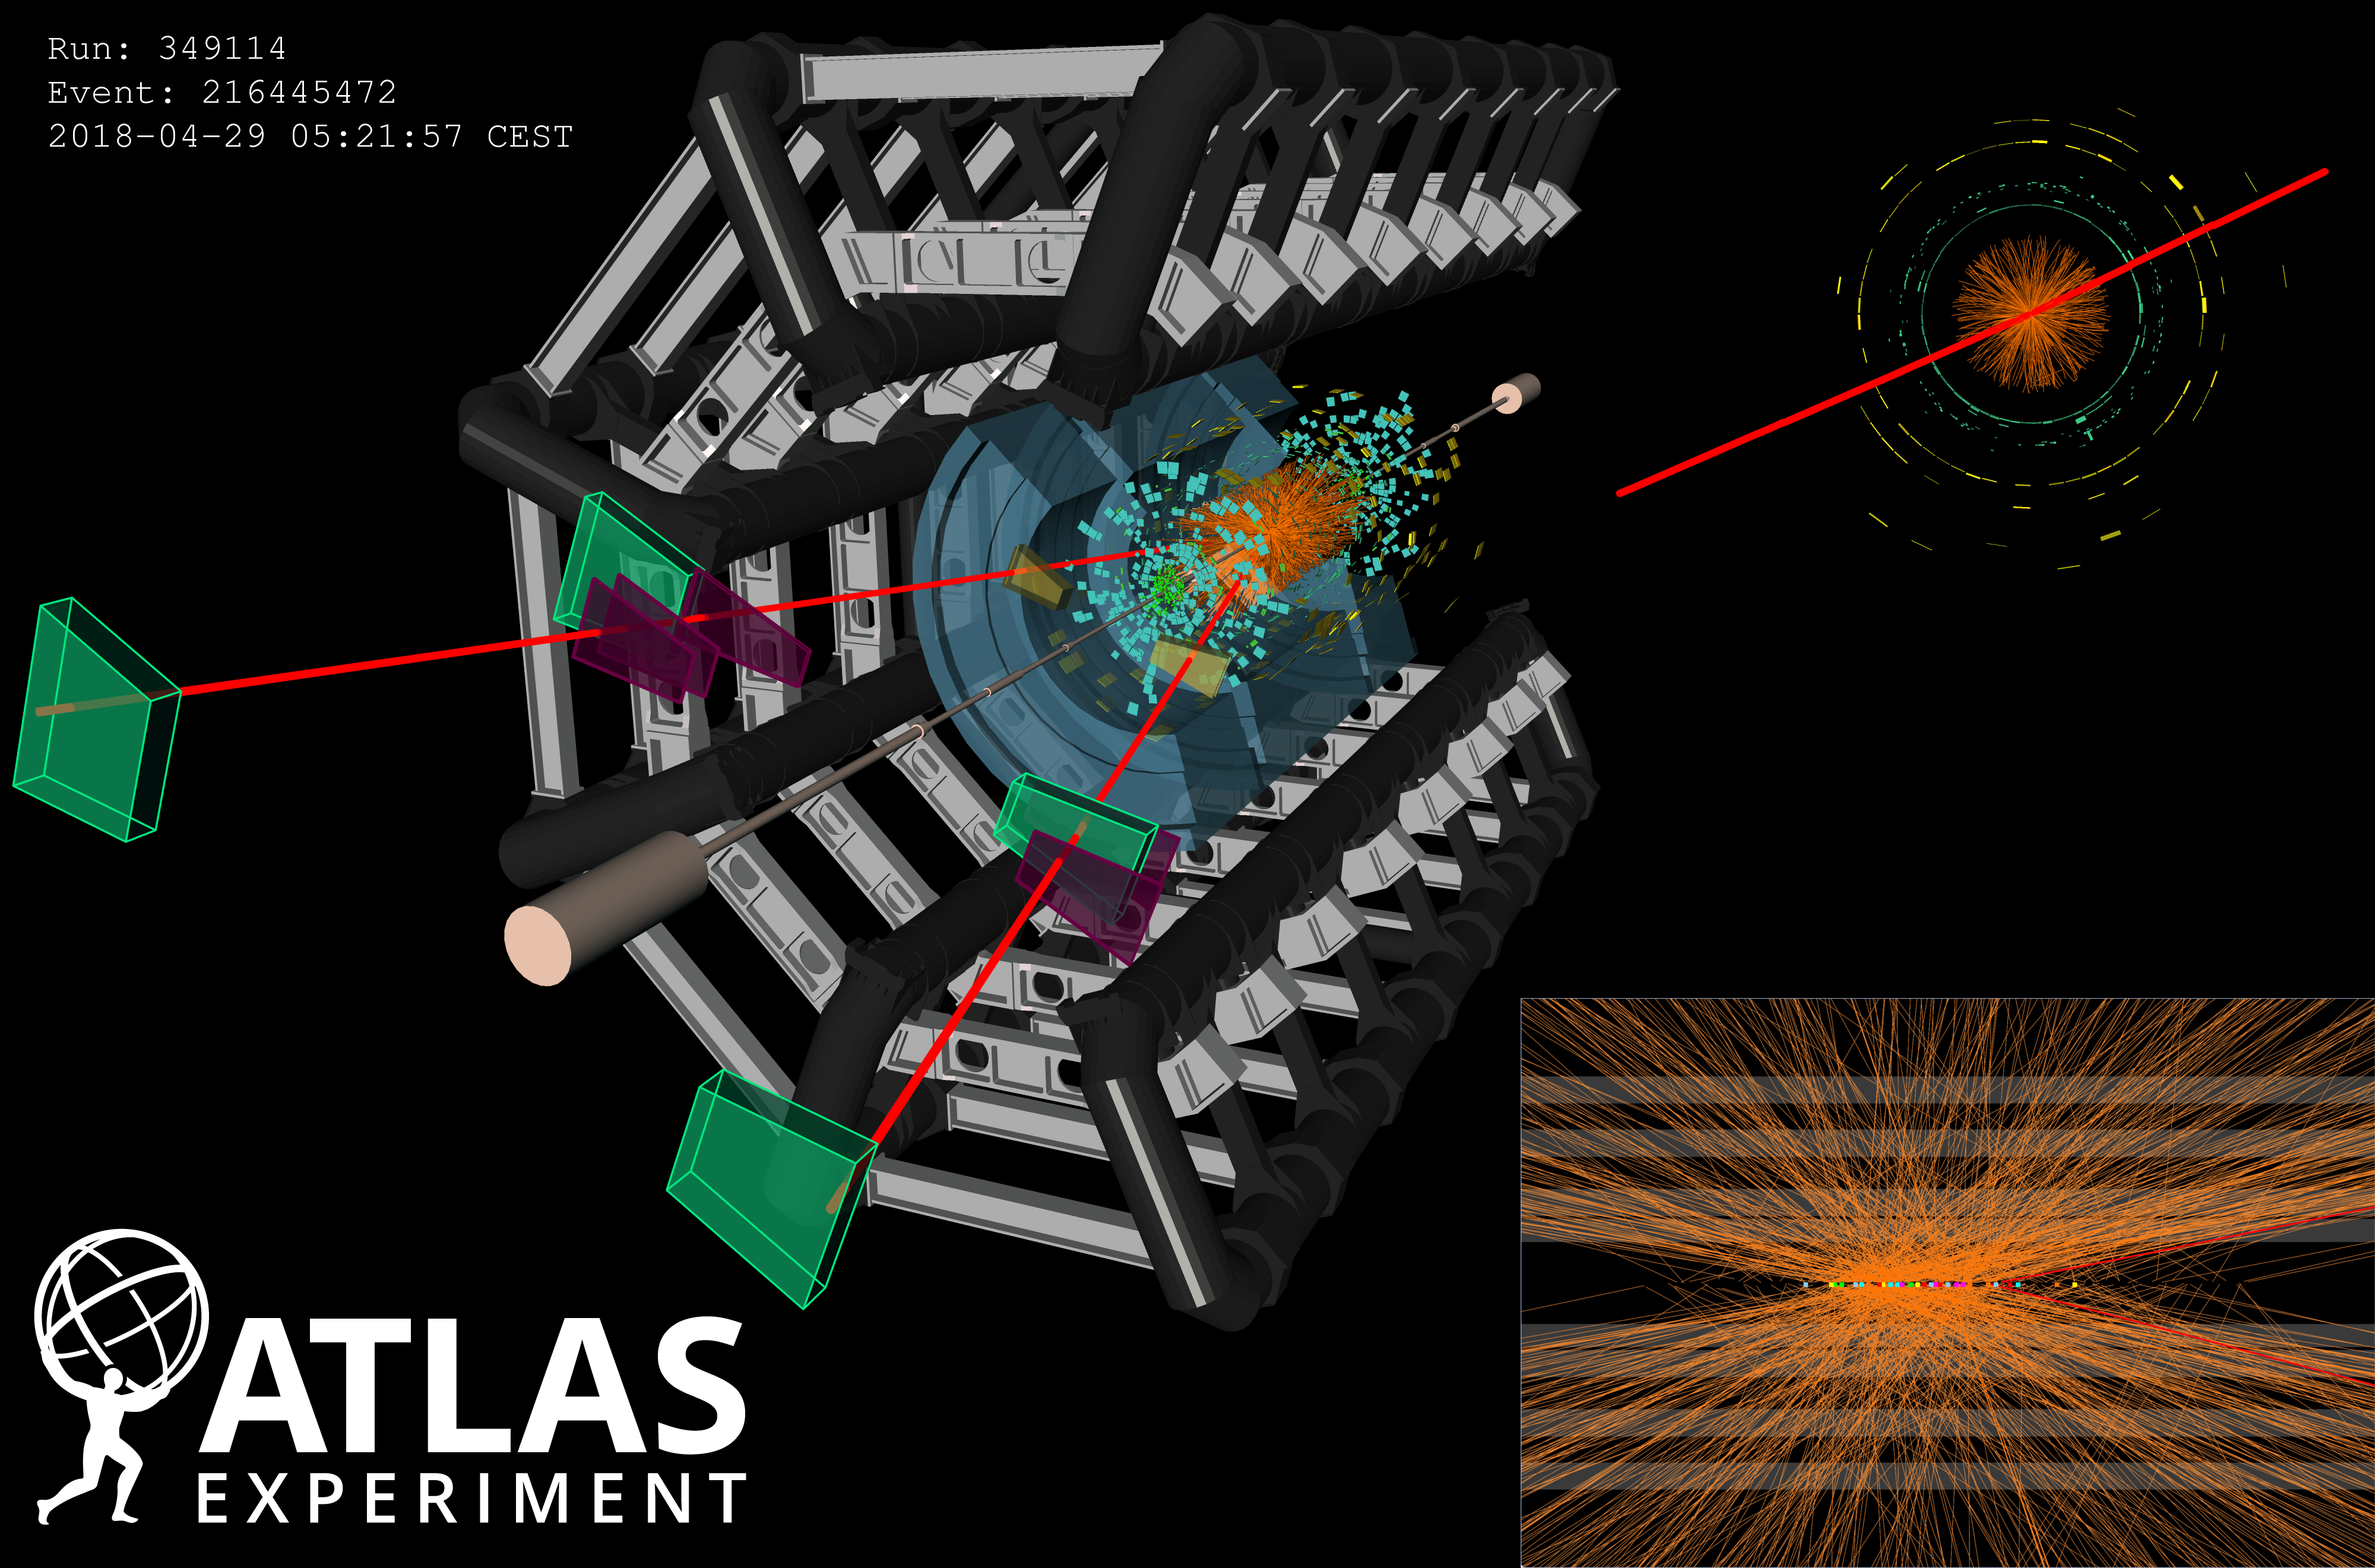
\includegraphics[width=.7\columnwidth]{../ThesisImages/LHCImages/28VertexPileup.png}
	\caption{ A candidate dimuon event ($Z\rightarrow \mu^+ \mu^-$) with 28 reconstructed verticies collected in 2018 with the ATLAS detector.
	}
	\label{fig:HighPileup}
\end{figure}

\begin{figure}[h!]
	\centering
	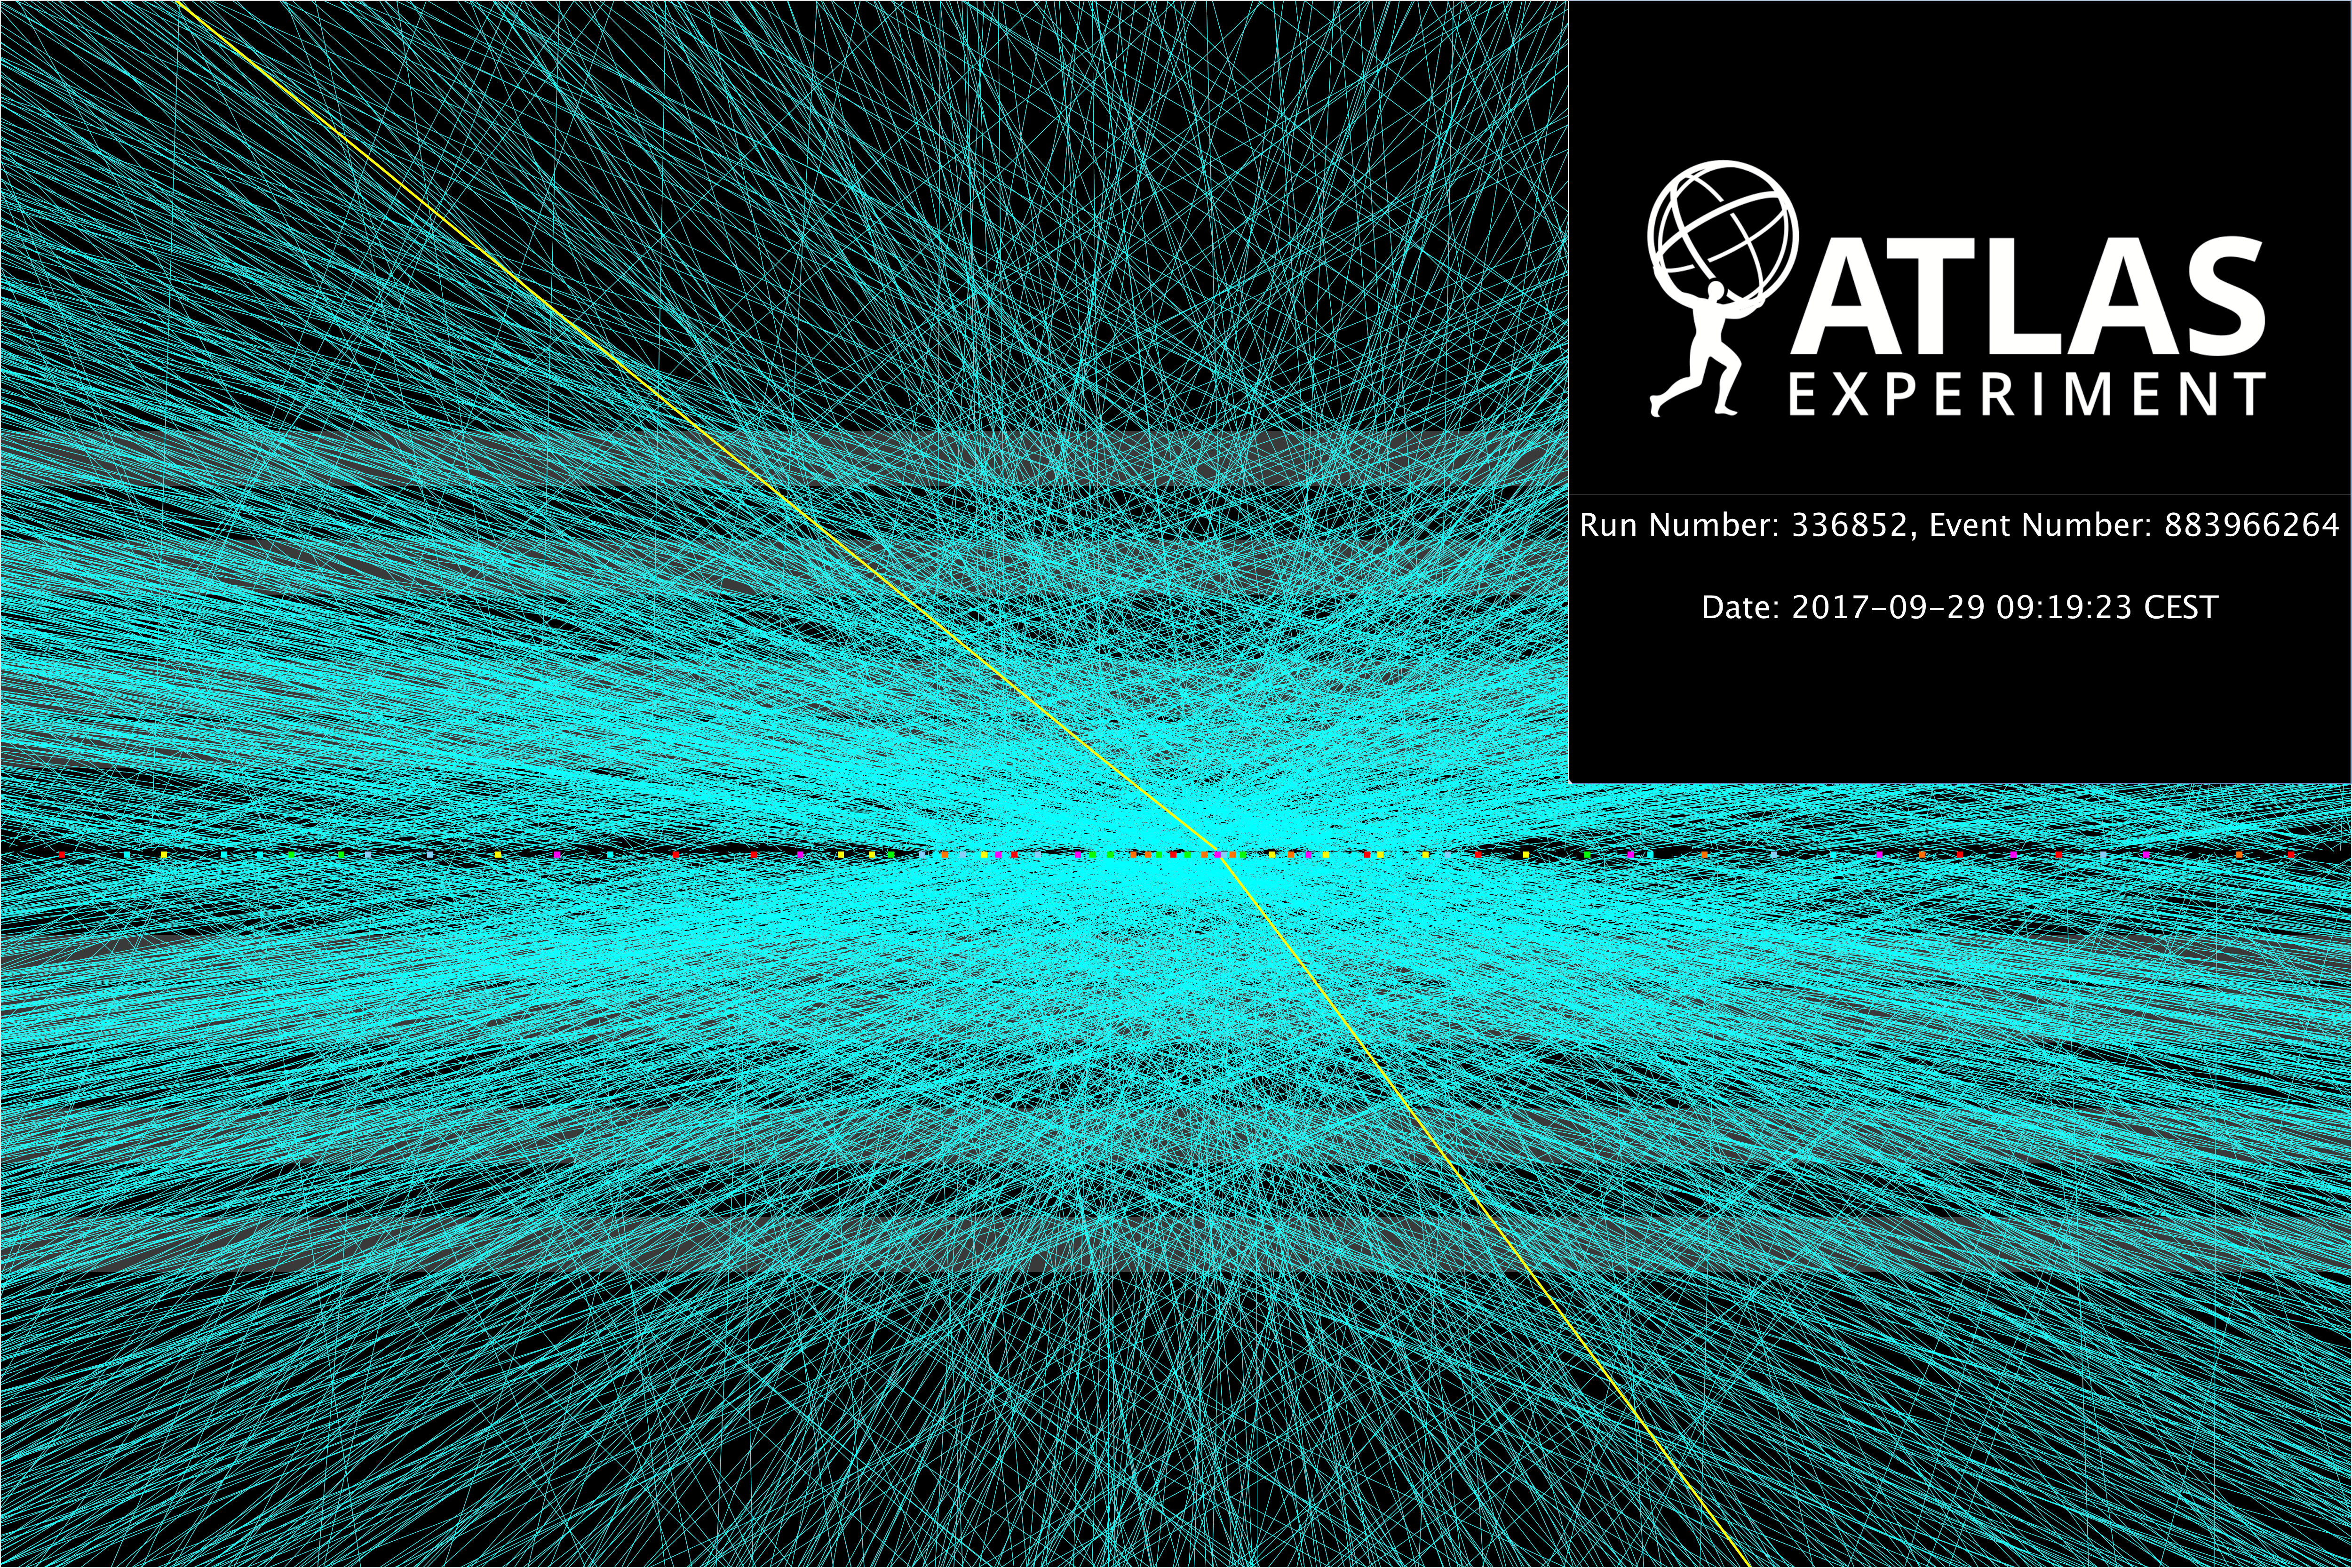
\includegraphics[width=.7\columnwidth]{../ThesisImages/LHCImages/65VertexPileup.png}
	\caption{ A candidate dimuon event ($Z\rightarrow \mu^+ \mu^-$) with 65 reconstructed verticies collected in 2017 with the ATLAS detector.
	}
	\label{fig:HighPileup2}
\end{figure}

\section{The ATLAS Detector}
\label{sec:ATLAS}
The ATLAS dectector, depicted in Figure \ref{fig:ATLASOverview}, is one of the two general-purpose detectors at the LHC.  It is the largest detector of its kind ever built at 46 meters in length, 25 meters in diameter, weighing 7000 tons, and containing around 3000 kilometers of cables\cite{ATLAS}.  Around the interaction points within the detector the ATLAS detector covers nearly the entire solid angle and is nominally symmetric.  ATLAS is built up of a variety of concentric subsytems, which will be discussed throughout this section, each with a specialized task and optimized for the measurement of different particle signatures.  
\begin{figure}[h!]
	\centering
	\includegraphics[width=\columnwidth]{../ThesisImages/LHCImages/AtlasDetector.png}
	\caption[Schematic of the ATLAS detector.]{Schematic of the ATLAS detector.\cite{ATLAS}
	}
	\label{fig:ATLASOverview}
\end{figure}
The primary subsystems used to measure particle trajectories and momenta accurately are the inner detector (Section \ref{sec:InnerDet}), the hadronic and electromagnetic calorimeters (Section \ref{sec:EMHCal}) and the muon system (Section \ref{sec:MuCal}).  The inner detector measures the paths of charged particles, called tracks.  The electromagnetic and hadronic calorimeters measure the energy of charged and neutral particles. The muon system measures the momenta of minimum ionizing particles (MIPs).  How various particles interact within these subsystems is shown schematically in Figure \ref{fig:ATLASInteractions}.
In addition to the various detectors and calorimeters the ATLAS detector has a magnet system (Section \ref{sec:ATLASMagnet}) which bends charged particles in the detector allowing for a measurement of their charge and momentum and distingushing them from neutral particles.  Between the inner detector and the calorimeters is a solenoid which provides an axial magnetic field.  Between the calorimeters and the muon system is a toroidal maget, from which ATLAS got its original acronym (\textbf{A} \textbf{T}oroidal \textbf{L}HC \textbf{A}pparatu\textbf{S}).

\begin{figure}[h!]
	\centering
	\includegraphics[width=\columnwidth]{../ThesisImages/LHCImages/ParticleInteractions.jpg}
	\caption[Cross section of a simulated ATLAS detector showing how various particles interact with ATLAS subsystems.]{Cross section of a simulated ATLAS detector showing how various particles interact with ATLAS subsystems.  Solid lines indicate interactions while dashed lines indicate that no interactions typically occur in that section of the detector. \cite{ParticleInteractions} 
	}
	\label{fig:ATLASInteractions}
\end{figure}


\subsection{Common Detector Variables and the ATLAS Coordinate System}
The ATLAS detector uses a right-handed coordinate system with the origin at the interaction point.  In a Cartesian coordinate system the z-axis is defined to be along the beam pipe (positive towards LHC Point 8) while the x-axis points toward the center of the LHC ring which means the positive y-axis points upwards as shown in Figure \ref{ATLASCoords}.  In practice coordinates used are a modified polar coordinate system.  In the transverse (xy-)plane to the beam line the azimuthal angle, $\phi$, is measured around the beam axis and radius, $r$, are used.  Away from the transverse plane the pseudorapidity, $\eta$, is defined by the polar angle (from the y-axis), $\theta$, to be $\eta= -\text{ln}[\text{tan}(\theta/2)]$.  Differences in $\eta$ are Lorentz invariant under longitudinal boosts such that the differences in the rest frames of colliding particles are not important for massless particles.  Since the particles typically present in the ATLAS detector are highly energetic, therefore have a large boost, the pseudorapidity is a good estimate of the true rapidity of the particles.  Massless particles are also produced uniformly in $\eta$ and not the polar angle $\theta$ which is why $\eta$ is preferred.

\begin{figure}[h!]
	\centering
	\includegraphics[width=0.5\columnwidth]{../ThesisImages/LHCImages/ATLASCoords.png}
	\caption[Coordinate system used in the ATLAS Collaboration.]{Coordinate system used in the ATLAS Collaboration.\cite{ATLASCoords}
	}
	\label{fig:ATLASCoords}
\end{figure}

The distance between any two objects within the ATLAS detector can be described geometrically by the variable $\Delta R = \sqrt{\Delta \eta^2 + \Delta \phi^2}$.  Another common variable used it the missing transverse energy, $E^{\text{miss}}_T$.  The information known about the missing energy is limited to the transverse plane because the momenta of the colliding particles is unknown along the beamline (only single quarks or gluons out of collection making up any beam proton interact).




\subsection{Magnet Setup}
\label{sec:ATLASMagnet}

The ATLAS detector has two magnet systems of note.  The first is the superconducting solenoid that surrounds the inner detector with a magnetic field aligned with the beam axis.  The solenoid has a magnetic field of 2T that makes the tracking of charged particles possible with the inner detector.  This magnet is a thin single layer coil, which is imperative to minimize the amount of material in front of the calorimeters. 

The toroid system consist of two parts, the end-cap and the barrel magnets.  The indings of these magnets is shown in Figure \ref{fig:ATLASMagnetWinding}.  Each of these magnets consist of eight superconducting air-core coils, together weighing 830 tons.  The end-cap coils are interleaved with the barrel coils.  A peak magnetic field strength of 3.9T (4.1T) is acheived in the barrel (end-cap) toroid which assist in the track and momentum measurement of high energy muons as they leave the ATLAS detector.  The barrel toroids covers a range of $|\eta|<1.4$ while the endcap toroids cover the range $1.6 < |\eta| <2.7$.  The remaining region is covered by a combination of the field of the two sets of toroids.
\begin{figure}[h!]
	\centering
	\includegraphics[width=0.7\columnwidth]{../ThesisImages/LHCImages/ATLASMagnetWinding.png}
	\caption[Schematic of the windings of the ATLAS magnet.]{Schematic of the windings of the ATLAS magnet.\cite{ATLAS}
	}
	\label{fig:ATLASMagnetWinding}
\end{figure}

%\subsection{SubDetectors}
\subsection{Inner Detector}
\label{sec:InnerDet}
The inner detector sits inside the solenoid magnet and is used to reconstruct charged particle tracks as they bend due to the magnetic field.  The inner detector is made up of four distinct parts.  The Insertable B-Layer (IBL) \cite{Capeans:1291633}, the Pixel Detectors, the Semiconductor Tracker (SCT), and the Transition Radiation Tracker (TRT)\cite{CERN-LHCC-97-016}.  The inner detector provides complete coverage for charged particle tracking, extending to $|\eta|<2.5$.  Momentum resolution as well as primary and secondary vertex measurements are done using the inner detector.  Secondary verticies are important and used in the identification of particles with delayed decays such as bottom quarks (Section \ref{sec:bjetReco}), charm quarks, and tau leptons. A schematic of the inner detector can be seen in Figure \ref{fig:ATLASInnerDet}.

\begin{figure}[h!]
	\centering
	\includegraphics[width=0.8\columnwidth]{../ThesisImages/LHCImages/ATLASInnerDetector.png}
	\caption[Schematic of the ATLAS inner detector.]{Schematic of the ATLAS inner detector.\cite{ATLAS}
	}
	\label{fig:ATLASInnerDet}
\end{figure}

The IBL was added during Long Shutdown I (2016) of the LHC and is closer to the interaction point than the innermost layer in Run 1.  This required adding a smaller beam pipe (reduction in radius from 29 mm to 25mm) but was able to improve the resolution of verticies and thus improve the reconstruction of events involving bottom quark decays as well as allowing for charm quark decays to be classified better than ever before.  This improvement is shown in Figure \ref{fig:impParamIBL} in a study of the impact parameter resolution.  The IBL functions as a fourth layer of the Pixel Detector and uses planar sensors (similar to the Pixel Detector) as well as 3D sensors which allowelectrons to interact with the bulk of the sensor as opposed to just the surface. 

\begin{figure}[h!]
	\centering
	\includegraphics[width=0.5\columnwidth]{../ThesisImages/LHCImages/tracking.png}
	\caption[Unfolded transverse impact parameter resolution measured with (Run 2) and without (Run 1) the IBL as a function of $p_T$.]{Unfolded transverse impact parameter resolution measured with (Run 2) and without (Run 1) the IBL as a function of $p_T$.\cite{Takubo:2017wvt}
	}
	\label{fig:impParamIBL}
\end{figure}

The next layer from the beam pipe, as detailed in Figure \ref{fig:ATLASInnerDet}, is the Pixel Detector which is a series of high granularity silicon pixel detectors which measure a position when a charged particle passes through them.  These silicon pixels are n-doped silicon wafers biased with a high voltage that will allow for the creation of electron hole pairs.  The electron then drifts toward the electrode which creates the position signal in the readout electronics.  In addition to the IBL there are three more cylindrical layers which are designed to ensure single pixel isolation and minimize leakage.  The pixels are $50 \times 400\mu\text{m}^2$ .  For complete coverage to the cylindrical system endcaps are placed on each side of the central barrel.  These endcaps consist of four wheels which have trapezoid shaped silicon pixels.  The three barrel layers consist of 67 million pixels and the endcaps total an additional 13 million pixels.
After the Pixel Detector is the Semiconductor Tracker (SCT) which is also made up of barrel and endcap detecors.  The barrel SCT is four cylindrical layers of silicon microstrip trackers where the endcaps are nine discs on each side of the barrel made up of either silicon or galium arsenide semiconductors.  The SCT contains over $60\text{m}^2$ of silicon detectors with over 6 million readout channels..

\begin{figure}[h!]
	\centering
	\includegraphics[width=0.5\columnwidth]{../ThesisImages/LHCImages/ATLASInnerStructure.png}
	\caption[Blown up schematic of the ATLAS inner detector with more detail.]{Blown up schematic of the ATLAS inner detector with more detail.\cite{Potamianos:2016ptf}
	}
	\label{fig:ATLASInnerDet}
\end{figure}

The final part of the Inner Detector is the Transition Radiation Tracker (TRT) \ref{Mindur:2017nqn}.  The TRT is a straw detector surrounding the SCT.  Every straw is a 4 mm in diameter Kapton tube with a 0.03 mm diameter gold-plated tungsten wire in its center.  In the barrel region there are 50,000 straws that are each 144 cm long and an addition 250,000 straws in both endcaps which are 39 cm in length.  Each straw is filled with an active gas mixture made up of mostly Xenon or Argon
When charged particles traverse across the TRT straws they ionize the active gas mixture and produce ionization clusters which depend on how far they traveled through the TRT (5-6 clusters per mm).  The straw walls are held at a high negative voltage such that the primary electrons are acclerated toward the gold-plated tungsten wire anode creating more ionization by liberating more electrons from the active gas and producing a detectable signal which is amplified and read out.  Trasition radiation occurs when a particle makes a transition between materials with different dielectric constants and the energy radiated is directly proportional to the Lorentz factor of the particle.  This allows for an excellent discrimination between electrons and charged pions.



\subsection{Electromagnetic and Hadronic Calorimeters}
\label{sec:EMHCal}
While the inner detector focuses on tracking the charged particles as they pass through the detector the ATLAS Calorimeter system is designed to absorb and measure the energy of neutral and charged particles.  The exceptions being muons which are able to penetrate through the calorimeters into the muon and neutrinos which do not interact at all within the ATLAS detector.  The calorimeters can be broken down into two major systems, the Liquid Argon (LAr) calorimeter\cite{CERN-LHCC-96-041} and the tile calorimeter (TileCal)\cite{CERN-LHCC-96-042}.  Both of these systems are shown in Figure \ref{fig:ATLASCaloSys}.

\begin{figure}[h!]
	\centering
	\includegraphics[width=\columnwidth]{../ThesisImages/LHCImages/ATLASCaloSystem.png}
	\caption[Schematic of the ATLAS hadronic and electromagnetic calorimeter systems.]{Schematic of the ATLAS hadronic and electromagnetic calorimeter systems.\cite{ATLAS}
	}
	\label{fig:ATLASCaloSys}
\end{figure}

The LAr calorimeter is a sampling calorimeter.  Sampling calorimeters use alternating layers of a dense absorbing material and an active material to measure the signal produced by showering particles.  The LAr calorimeter uses lead as the absorbing material and the active material is liquid argon and measured with copper-tungsten sensors.  The layers in the LAr calorimeter are arranged in an "accoridan-shaped" geometry shown in Figure \ref{fig:LArAccordian} to provide complete azimuthal coverage.  This allows for the electromagnetic energy resolution to be uniform in the azimuthal direction.  The issue with a sampling calorimeter is that it does not directly measure the entire energy of the particle, only the interactions that occur in the active layers.  Sampling also means that youre subjected to sampling statistics in that large fluctuations can occur through an electromagnetic shower that are are not measured correctly because of the absorber.  
\begin{figure}[h!]
	\centering
	\includegraphics[width=0.5\columnwidth]{../ThesisImages/LHCImages/LArAccordian.png}
	\caption[Sketch of the accordian structure used in the LAr Calorimeter]{Sketch of the accordian structure used in the LAr Calorimeter.\cite{CERN-LHCC-96-041}
	}
	\label{fig:LArAccordian}
\end{figure}

For sampling calorimeters it is important to know the ratio $\frac{E_{\text{visible}}}{E_{\text{deposited}}}$ so that you can reconstruct the energy of a particle based on only the energy measured by the active layers.  This ratio must be measured with test beams where the original beam energy is known precisely.  Sampling calorimeters do allow the complete detection of electromagnetic showers as there is a large amount of material to traverse through so all of the energy can be deposited within the detector. The amount of material travesed by each particle is an important aspect as it includes not only the active material and absorber but also the support structures and cables which can play a role in particle interactions.  The thickness of of material passed through is typically measured in radiation lengths ($X_0$), where an electron passing through one radiation length will lose 1/e of its energy to bremsstrahlung.  The amount of radiation lengths in the LAr calorimeter is shown in Fugre \ref{fig:MaterialBudget}.  

\begin{figure}[h!]
	\centering
	\includegraphics[width=\columnwidth]{../ThesisImages/LHCImages/MaterialBudget.png}
	\caption[Number of radiation lengths throughout the LAr calorimeter as a function of $|\eta|$]{Number of radiation lengths throughout the LAr calorimeter as a function of $|\eta|$\cite{ATLAS}
	}
	\label{fig:MaterialBudget}
\end{figure}

Forward from the barrel there are two electromagnetic endcap (EMEC) wheels with a similar accordion structure to the modules in the barrel that cover ranges $1.4<|\eta|<2.5$ and $2.5<|\eta|<3.2$.  Outside of the EMEC wheels it the LAr hadronic endcap (HEC) with a simpler parallel plate structure.  The last part of the LAr calorimeter is the LAr forward calorimeter (FCal).  Due to the FCal's proximity to the beamline the particle flux is very high so a dense calorimeter is used to avoid losing energy into other pieces of the detector.  The FCal is made up of three layers the first is copper and the others are tungten.  

The remaining calorimeter system is the TileCal which is primarily responsible for hadronic calorimetry in the central region $|\eta|<1.7$.  TileCal is also a sampling calorimeter with iron plate absorbers and plastic scintillating tiles. The scintillating tiles are placed orthogonal to the beamline and readout using wavelength shifting fibers connected to photomultiplier tubes on the outside of the system.  TileCal has a fixed central barrel and two extended barrel sections as shown in Figure \ref{fig:ATLASCaloSys}.  The extended barrel sections can be moved.  The total nuclear interaction length of the TileCal is $7.4\lambda$ where $\lambda$ is the mean distance a hadronic particle will travel before experiencing an inelastic interaction with the material it is traveling through.  The total interaction length for each section of the calorimeter is shown in Figure \ref{fig:InteractionLengths}.


\begin{figure}[h!]
	\centering
	\includegraphics[width=0.8\columnwidth]{../ThesisImages/LHCImages/InteractionLengths.png}
	\caption[Number of interaction lengths throughout the LAr calorimeter as a function of $|\eta|$]{Number of radiation lengths throughout the LAr calorimeter as a function of $|\eta|$\cite{ATLAS}
	}
	\label{fig:InteractionLengths}
\end{figure}


\subsection{Muon System}
\label{sec:MuCal}
The final and outermost subdetector of the ATLAS detector is the muon spectrometer, which measures the momentum of muons.  Different technologies are used in the barrel and endcap regions for both measurement and triggering (deciding which events to keep when only a small fraction of events can be recorded).  For the barrel region, $|\eta|<2.7$, three layers of Monitored Drift Tubes (MDT) are used for precision energy and tracking measurements and Resistive Plate Chambers (RPC) for triggering.  In the forward region, $2.0<|\eta|<2.7$ , where the flux is higher Cathode Strip Chambers (CSC) are used for energy and position measurements and Thin Gap Chambers (TGC) are used for triggering.  These systems, shown in Figure \ref{fig:ATLASMuonSys} are aided by the magnetic field created by the toroid system discussed in Section \ref{sec:ATLASMagnet}.
\begin{figure}[h!]
	\centering
	\includegraphics[width=\columnwidth]{../ThesisImages/LHCImages/ATLASMuonSystem.png}
	\caption[Schematic of the ATLAS muon detector.]{Schematic of the ATLAS muon detector.\cite{ATLAS}
	}
	\label{fig:ATLASMuonSys}
\end{figure}

MDTs are arranged in chambers of up to 6 layers of aluminum tubes ranging in length from one to six meters.  Each tube is 30 mm in diameter and contains a sense wire $50\mu\text{m}$ in diameter.  The chambers are arranged with a support spacer in between layers of MDTs that have a built-in optical sensor to monitor the drift tubes (hence the name) for deformations.  This ensures the precision of measurements does not change over time.  The MDTs are only used in the barrel and not the forward region because they are inappropriate in areas with high rates, in this case a high flux of muons. 

For the forward region CSCs are used.  CSCs consist of arrays of positively charged wires crossed with negatively charged strips within a gas.  As muons pass through they knock electrons from atoms in the gas which go toward the anode wires. Since the strips and wires are perpendicular to each other two position coordinates are read out.  CSCs have the benefit of giving good single and two-track resolution in a high flux environment.

The trigger system for muons in the barrel region uses RPCs which are parallel plates with opposite charge separated by a gaseous volume. A muon passing through an RPC knocks electrons from the gas which cause an avalance of electrons which do not get picked up by the electrode but instead by external metal strips.  The pattern of metal strips that gets hit gives a quick measurement of the muon momentum which is used by the trigger to make the immediate decision about the event.
The endcap muon trigger relies on TGCs.  TGCs are anode wires with graphite cathods in between thin layers of fiberglass laminate.  Similarly to why CSCs are used over MDRs in the forward region TGCs have excellent timing resolution and can handle the high flux of muons in the forward regions.


\subsection{Trigger and Data Acquisition}
\label{sec:TDAQ}
The amount of data the LHC is capable of producing is staggering and the ATLAS trigger system is required to reduce the enormous amount of data produced to a reasonable amount while keeping the most interesting events.  The LHC provides collisions at a rate of 40MHz.  Every event saved to tape requires about 1.6MB of space \cite{Outreach:1457044}. To keep all of the data produced 64TB/s would need to be saved or 230PB of data for a 12-hour run or 400EB of data per year (150 days of uptime). 

In order to reduce this to a level that can actually be dealt with the ATLAS trigger system uses a two level trigger system.  A hardware trigger, Level 1 or L1 trigger, is used to lower the rate from 40MHz to between 75 and 100kHz which is sent to the next level of the trigger system, the High Level Trigger (HLT).  Another factor of 50 in rate reduction is achieved by this software based HLT to reduce the rate below 2kHz.  A flowchart of the ATLAS trigger and data acquisition system is shown in Figure \ref{fig:ATLAStdaq}.  When combined with partial event readouts and the $<$2kHz full event readout the total bandwidth requirement is around 3GB/s to be written.  This means that only around $0.004\%$ of data is stored.
\begin{figure}[h!]
	\centering
	\includegraphics[width=\columnwidth]{../ThesisImages/LHCImages/ATLASTDAQR2.png}
	\caption[Flow diagram of the ATLAS trigger and data acquisition system used in Run 2.]{Flow diagram of the ATLAS trigger and data acquisition system used in Run 2.\cite{ATLASTDAQ}
	}
	\label{fig:ATLAStdaq}
\end{figure}

\subsubsection{Level 1 Calorimeter}
The Level 1 hardware trigger uses coarse information from some of the subdetectors.  Information from the calorimeters is sent to the Level 1 Calorimeter (L1 Calo) system.  L1 Calo uses low granularity information to identify Regions of Interest (RoIs) from objects that interact in the calorimeters (photons, electrons, jets, taus), events with high total energy, as well as events with an imbalance of energy coming from missing transverse energy.  The information is fed into the L1 Calo system and put through a preprocessor that allows L1 Calo to handle the effects within ATLAS from pileup events.
Information from TileCal and the trigger portions of the muon systems goes to the Level 1 Muon (L1 Muon) system which applies various logical processes to determine if an event should be kept.  
Outputs from L1 Calo and L1 Muon are passed to the Central Trigger Processor (CTP) which provides a level 1 trigger accept and LHC timing information to the detector read out.  At the same time the CTP gives RoIs to the HLT.

\subsubsection{High Level Trigger}
The HLT takes RoIs from the CTP as well as full detector granularity and makes a further decision if that event should be saved.  This is done using a computing farm of over 40,000 cores that run over 2,500 independent algorithms (trigger chains) on the RoIs.  The HLT can provide partial and full event reconstruction depending on the event stream the event is decided to be within.  The main event stream is the physics analysis stream which gets full event reconstruction but other the other streams typically only require partial event reconstruction.  The other streams are used for a variety of things such as trigger level analysis, monitoring of the subsystems, or calibrating the detector.
%\subsubsection{Data Farm Information}
%\subsubsubsection{Trigger Rates}
%\subsubsubsection{Amount of Data}


%%%%%%%%%%%%%%%%%%%%%%%%%%%%%%%%%%%%%%%%%%%%%%%
%%%%%%%%%%%%                                                                                                   %%%%%%%% 
%%%%%%%%%%%%                           BEN                                                                  %%%%%%%% 
%%%%%%%%%%%%                                                                                                   %%%%%%%% 
%%%%%%%%%%%%%%%%%%%%%%%%%%%%%%%%%%%%%%%%%%%%%%%
%The particle physics program at CERN uses some of the most complex machines ever built, and have required the efforts of thousands of people to design, commission, and maintain.  This section outlines the systems which are used to provide the collisions and measure their products.
%
%\section{The Large Hadron Collider}
%
%The Large Hadron Collider (LHC) is the worlds largest and most powerful particle accelerator, at over 27\,km in circumference and capable of accelerating protons a center of mass energy of 13\,TeV.  It is located 100 meters underground along the French-Swiss border at CERN, just outside Geneva, Switzerland.  The beams are brought to collisions at different points along the ring to four major experiments: ATLAS~\cite{ATLAS}, CMS~\cite{CMS}, ALICE~\cite{ALICE}, and LHCb.\cite{LHCb}
%
%Protons in the LHC start as hydrogen gas which is ionized, the protons of which are accelerated to 50\,MeV by the LINAC2 linear accelerator.  From here, particles are accelerated in a series of circular accelerators of increasing size, starting with the Proton Synchrotron Booster which raises their energy to 1.4\,GeV.  This is followed by the Proton Synchrotron (PS) (25\,GeV) and Super Proton Synchrotron(SPS) (450\,GeV), after which proton bunches are finally injected into the LHC where they are ramped up to their final collision energy.  For Run 1, the LHC operated $\sqrt{s}$ = 7 and 8\,TeV, while in the ongoing Run 2 at $\sqrt{s}$ = 13\,TeV.  The CERN accelerator complex is shown in Figure~\ref{fig:AcceleratorMap}.
%
%\begin{figure}[h!]
%	\centering
%	\includegraphics[width=\columnwidth]{figures/Detector/CERNAcceleratorComplex.jpg}
%	\caption{Schematic of the CERN accelerator complex.\cite{DeMelis:2119882}
%	}
%	\label{fig:AcceleratorMap}
%\end{figure}
%
%\subsection{Bunches and bunch trains}
%
%The LHC operates at a radio frequency (RF) of 400\,MHz which can be filled with bunches every 10 RF buckets for a separation of 25\,ns between bunches.\cite{Boussard:410377}  During Run 1 and the early part of Run 2 the LHC operated with 50\,ns spacing to reduce the effect of the electron cloud, but moved to the design spacing of 25 ns for the remainder of Run 2 data taking at the insistence of the detector collaborations.  This spacing, coupled with the $\sim27$\,km circumference of the LHC, means there are 3564 bunches which could be filled in the ring at any time.  In practice the LHC never fills all of these bunches at once, but instead the bunches are organized into $trains$.
%
%Bunch trains are groups of sequentially filled bunches in the machine and are driven by the design of the PS and SPS rings.  For a typical 2016 run, a single injection from the PS to the SPS was 72 sequential bunches, while the SPS transferred 288 bunches (4$\times$72) at a time over to the LHC.\cite{Bartmann:IPAC2017-TUPVA007}  The gaps between each of these bunches are driven by the kicker magnet rise times for each of these systems.  The minimum kicker times for the PS and SPS are 200\,ns and 800\,ns respectively, so each 72 bunch train is separated by 8 empty bunches, and each grouping of 288 is separated by 32 empty bunches.  The filling scheme also includes an abort gap, a space of approximately 100 empty bunches which is used in the case that the beam needs to be redirected to the beam dump.  In total, the number of filled bunches in the machine caps out around 2800 at a time.
%
%While the overall luminosity can be directly increased by upping the number of bunches in the machine at one time, the LHC has also tested other filling schemes which reduce the number of filled bunches but increase the charge in each bunch, or decrease the beam emittance, leading to a higher instantaneous luminosity and overall integrated luminosity.
%
%\section{The ATLAS Detector}
%
%The ATLAS detector is a multipurpose physics detector, located at Point 1 on the LHC ring near the main CERN site.  ATLAS weighs in at around 7000 tons, and is 44\,m long and 25\,m in diameter.  The detector is composed of multiple layers which measure their own unique portions of the collision products, which are described in the following section.  Figure~\ref{fig:AtlasDetector} shows how these systems are laid out.
%
%\begin{figure}[h!]
%	\centering
%	\includegraphics[width=\columnwidth]{figures/Detector/AtlasDetector.png}
%	\caption{A cutaway view of the ATLAS detector showing the various components.\cite{ATLAS}
%	}
%	\label{fig:AtlasDetector}
%\end{figure}
%\subsection{Coordinate System}
%
%The ATLAS experiment uses a right-handed coordinate system, with the origin at the nominal interaction point (IP) in the center of the detector.  The x-axis points from the IP towards the center of the LHC ring, and the y-axis points upward towards the surface.  ATLAS uses a cylindrical coordinate system which defines a radial distance $r = \sqrt{x^2+y^2}$ and azimuthal angle $\phi$ around the z-axis.  Instead of using the polar angle from the beamline $\theta$, pseudorapidity is typically used, defined as $\eta = -\ln{(\tan{\frac{\theta}{2}})}$.
%
%Massive objects, such as jets, are measured to have a rapidity defined as $ y = \frac{1}{2}\ln{\frac{E+p_z}{E-p_z}}$.  In the limit where $\pt \gg m$, as is often the case in this search, $y \approx \eta$, meaning that the rapidity of a jet and its detector location given by pseudorapidity are approximately interchangeable.  Differences in rapidities are Lorentz-invariant under z-axis boosts, making them useful for measuring if two jets are back-to-back in their rest frame.
%
%\subsection{Magnet System}
%
%ATLAS is composed of four separate magnets: one central solenoid encompassing the ID, one barrel toroid, and two endcap toroids.  The central solenoid provides a 2.0\,T magnetic field and is responsible for bending charged particle tracks near the IP to measure their momentum.  The namesake toroids provide a peak field of 4.0\,T, bending muons in a different plane than the solenoid field does to improve their momentum measurement.
%
%\subsection{Inner Detector}
%
%The ATLAS Inner Detector (ID) is comprised of three different subsystems: the silicon pixel layers (including the Insertable B-Layer (IBL) new in Run 2), the semiconductor tracker (SCT), and transition radiation tracker (TRT).  In total, the system covers the angular range $|\eta|<2.5$.  Information from all three subsystems is used to reconstruct tracks down to \pt = 0.4\,GeV.\cite{IDPerf}
%
%\subsubsection{Pixel and Semiconductor Trackers}
%
%The pixel detector system is composed of four concentric layers of silicon pixels, providing multiple high-resolution hits for charged particles traveling through.  The closest layer to the beampipe, the IBL, was added during Long Shutdown 1 (LS1) before the start of Run-2 operations.  At only 3.3\,cm away from the beamline, this additional tracking layer greatly improved the efficacy of tracking algorithms by an additional hit for tracks passing through multiple layers, and allowing for better resolution of secondary decay vertices, such as those originating from b-quarks.  The IBL also contains newer technologies than the rest of the pixel system which allow it to withstand the harsh radiation close to the beampipe.  This will allow the IBL to continue performing well as the innermost layer of the old pixel system degrades due to radiation, allowing for the maintenance of the current tracking performance.
%The SCT uses silicon microstrips and sits just outside the pixel system.  It is comprised of four barrel layers and 18 endcap disks (9 on each side of the detector), and range from 30 to 51\,cm from the beamline, adding additional position information for track finding.
%
%\subsubsection{Transition Radiation Tracker}
%
%The TRT operates on a very different principle than the other two tracking systems, taking advantage of the energy emitted when high energy particles transition between media with differing indices of refraction.  It is comprised of nearly 300,000 polyimide straws with an external aluminum layer and central gold-plated, tungsten wire at the center of each 4mm diameter tube.  The straws are filled with a gas mixture of Ar, CO$_2$, and O$_2$, and are ionized either by charged particles passing through or by emitted transition radiation.  Each straw hit provides additional 2-D hit information for track finding, as well as acting as a discriminant in electron identification.
%
%The TRT is scheduled to be removed as part of the ATLAS Phase-II upgrade starting in 2025, as the pileup conditions in Run 4 are expected to create TRT occupancies near 100\%, significantly degrading the performance of the system. The average TRT occupancy as a function of the number of interactions per crossing is shown in Figure~\ref{fig:TRTOccupancy}.  
%
%\begin{figure}[h!]
%	\centering
%	\includegraphics[width=0.6\columnwidth]{figures/Detector/TRTOccupancy.png}
%	\caption{Average track region TRT occupancy as a function of track $\eta$ using data taken during the 2015 and 2016 ATLAS runs for four different values of the average interactions per bunch crossing.
%	}
%	\label{fig:TRTOccupancy}
%\end{figure}
%
%\subsection{Calorimeters}
%
%ATLAS uses two different types of calorimeters to measure the energies of leptons, hadrons, and photons.  First is the liquid argon (LAr) electromagnetic calorimeter, which captures most of the energy from EM showers.  Second is the steel-scintillator Tile calorimeter which captures the energy from hadronic showers.  Optimal performance of the calorimeter systems under challenging conditions is vital to nearly every physics signature ATLAS searches for.  The system has nearly hermetic coverage in $\phi$ but is made up of several overlapping systems and varying thicknesses of material in $\eta$, and so special care must be taken to accurately calibrate the detector response in each region of the detector.
%
%The journey from calorimeter hits to the eventual trigger is discussed in detail in Chapter~\ref{ch:Calorimetry}.
%
%\subsubsection{Electromagnetic Calorimeter}
%
%The EM calorimeter uses liquid argon as an active medium, a choice motivated by the need for radiation-hardness, especially over the 30+ year run time of the LHC.  The calorimeter is composed of accordion shaped absorbers of lead with steel backing, with liquid argon flowing between and copper electrodes which measure the energy deposited.
%
%The LAr calorimeter is a sampling calorimeter, meaning that only a small fraction of the total energy from a particle traversing it is actually measured.  The power of an absorbing material is given by its radiation length ($X_0$), the distance an electron must travel in that material for its energy to be reduced by a factor of $\frac{1}{e}$.  Liquid argon is not dense enough as a medium to fit in a reasonable size calorimeter, and so lead (with a radiation length 20$\times$ shorter) is used to slow down the particles.  The EM calorimeter contains enough material to fully contain all but the largest electromagnetic showers, typically 25-30 interaction lengths depending on the region of the detector.  The actual pulse observed in the calorimeter is created when charged particles, showering from interactions in the absorber layers, cause the LAr to ionize and then release electrons which are accelerated by an electric field to the electrodes to become the calorimeter pulse.  The amount of energy actually measured by the LAr is much less than the total shower energy, and so it must be scaled back up by comparing the behavior of particles using test beam data where the incoming particle energy is well known.
%
%The EM Barrel covers the central region out to $|\eta|<1.475$, and two endcaps cover the range $1.375<|\eta|<3.2$.  The calorimeter is divided up into four layers of varying granularity, the first of which is the presampler.  This layer is closest to the inner tracker and has no absorber material in it, but instead is used to measure the amount of energy which has dissipated due to interactions with the material in the inner detector before it reaches the calorimeters.  The other three layers vary in thickness and granularity, and the values from each of these layers help determine the shape evolution of the shower as it progresses through the calorimeter, an important tool for electron/photon identification.  These pulses are read out and given to the level-1 trigger at coarse level, and if an event passes the trigger they are passed with full granularity to the high-level trigger.
%
%\subsubsection{Hadronic Calorimeter}
%
%Situated immediately outside the EM calorimeter, the hadronic calorimeter systems capture the remaining energy from hadrons which have already deposited a fraction of their energy in the EM layers.  The depth of material is characterized by the number of nuclear interaction lengths, the distance a hadron travels before undergoing an inelastic collision.  The depth varies as a function of $\eta$, but the hadronic calorimeters typically comprise 8-12 interaction lengths, enough to stop all but the most powerful showers.  In the barrel region, it is comprised of steel absorbing layers and scintillating polystyrene tiles, and the deposited energy is measured by molecular excitations in the scintillator emitting UV light which is then read out by photomultiplier tubes (PMTs).  The barrel systems covers the region $|\eta|<1.7$, but a different, more radiation-hard technique is required for the more forward regions.
%
%The Hadronic Endcap (HEC) covers the range $1.5<|\eta|<3.2$, and operates in largely the same manner as the EM systems.  Instead of the lead-steel combination of the EM layer, the HEC uses much thicker copper layers as the absorbers, with LAr still acting as the active medium.  The forward calorimeter (FCAL) covers the range $3.1<|\eta|<4.9$ and uses a combination of copper and tungsten plates as the absorbers.  Overall the hadronic calorimeters are much coarser than their EM counterparts, with a granularity of 0.1$\times$0.1 ($\Delta\eta\times\Delta\phi$) in the region $|\eta|<2.5$, and $0.2\times0.2$ in the forward regions.  
%
%\subsection{Muon Spectrometers}
%
%Muons interact very little with the calorimeters in ATLAS, leaving behind only tracks in the inner detector before they reach the outermost systems in ATLAS, the muon spectrometers.  In the muon systems, ATLAS's namesake toroids bend the tracks of passing muons to determine their momenta.  The muon system uses different technologies in the barrel and endcap regions, as well as different systems for triggering and momentum measurement.
%
%In the central region, monitored drift tubes (MDTs) are used to measure the tracks, and thus the momenta, of muons, while resistive plate chambers (RPCs) are used for triggering.  This split is required because of the long drift time of the MDTs of ~700\,ns, which is outside of the window the level-1 trigger system can use.  To deal with the higher backgrounds in the forward regions, cathode strip chambers (CSCs) are used for momenta measurements and thin-gap chambers (TGCs) are used for triggering.
%
%The muon system operates under the assumption that all other particles will be fully absorbed in the calorimeter layers, and thus any detected particles in the region must be muons.  However, in the case of very high-\pt jets some of the energy can "punch through" the calorimeters and register hits in the muon system.  This effect must be compensated for and is discussed later in the context of jet calibration.
%
%\subsection{Forward Detectors}
%
%Further down the beampipe from the IP are the various forward detectors for ATLAS which are primarily used for luminosity and cross-section measurements.  LUCID (LUminosity measurement using Cerenkov Integrating Detector) sits 17\,m down from the IP and consists of quartz fiber bundles connected to PMTs which detect Cherenkov radiation as charged particles pass through the quartz.  The multiplicity is proportional to the amount of interactions taking place at the IP, and is therefore used to measure the instantaneous luminosity.  ALFA (Absolute Luminosity For ATLAS) uses Roman Pots 240\,m from the IP to detect protons at angles very close to the beamline; ALFA is used in dedicated runs to measure the total proton-proton cross-section.  ZDC (Zero Degree Calorimeter) sits 140\,m from the IP and is used to measure the amount of neutral particles (neutrons and photons) left as beam remnants once the rest of the beam has been bent away by the steering magnets of the LHC; this information is used as a minimum-bias trigger for ATLAS, and as a centrality measurement for heavy-ion collision data.  Finally, AFP (ATLAS Forward Protons) is new for Run 2, primarily focusing on diffractive physics in special low-luminosity runs.
%
%\subsection{Trigger and Data Acquisition}
%During nominal operations, the LHC provides collisions at a rate of 40\,MHz, or an event every 25\,ns.  As each event is slightly under 2\,MB of data, this represents an extraordinary amount of information, and is far more than could be conceivably be written to disk, much less properly analyzed.  In order to reduce the data rate to a manageable level, and to ensure that only the events with the most interesting physics are saved, a two-tiered trigger system is used.
%\subsubsection{Level-1 Trigger}
%The level-1 (L1) trigger is hardware based, making decisions on whether or not to keep an event within 2.5\,$\mu$s.  For Run-2 operation, the L1 trigger reduces the event rate to a maximum of 100\,kHz.  The L1 trigger is made up of several subsystems which bring together decisions from different areas of the detector to make a final decision on whether or not to keep an event.
%
%The L1 calorimeter trigger (L1Calo) uses information from the EM and hadronic calorimeters in the form of rough 0.1$\times$0.1 ($\eta\times\phi$) trigger towers.  From this information, candidates for jets, electrons/photons, and taus are constructed and passed along as regions of interest (RoI) to the next stages in the trigger telling the type of object, its transverse momentum as measured at L1, and its location in the detector.  The amount of global missing transverse energy (MET) is also calculated and used as part of the trigger signature.  The L1Muon system uses a coincidence of hits in the RPCs and TGCs to identify muon candidates.  Since precision momentum information from the MDTs and CSCs takes too long for the L1 decision, the muon momentum is roughly estimated using the hit pattern, and then marked as being above one of a set number of \pt thresholds.
%
%Within each system, a list of pre-determined triggers are compared against the RoIs found in the event.  For example, the muon system has triggers for muons above 20\,GeV (L1\_MU20) as well as for two muons above 6\,GeV (L1\_2MU6).  The list of all triggers passed in each system is passed along to the Central Trigger Processor (CTP) where the final determination on whether or not to save an event is made.
%
%RoIs from both L1Calo and L1Muon are then sent to the L1 Topological trigger. (L1Topo)  Newly commissioned in 2016, L1Topo allows for more advanced combinations of trigger objects from the two systems, including operations such as invariant mass, angular separation between objects, and transverse mass.\cite{L1Topo}  This additional processing step greatly reduces the background rates for certain processes, allowing for much lower energy thresholds when using objects triggered from L1Topo.  Similar to L1Calo and L1Muon, the list of triggers passed by an event is passed along to the CTP.
%
%The CTP is the final stage of the L1 trigger.  It receives a list of all passed triggers from the other subsystems and compares it against an L1 trigger menu.  The trigger menu determines which triggers should be turned on or off during a given run, as well as the prescale, or rate reduction, rates for triggers.  Triggers with lower energy thresholds are often prescaled, meaning that only a fraction of events that pass a given trigger are kept.  For example, a physics menu item with a prescale of 20 will have only 1 out of 20 events that pass the trigger saved, while the other 19 times the event is not saved unless some other trigger is also passed and and marks the event for saving.  The L1 trigger menu evolves over the course of time as well as within a single physics run, changing the prescales of physics items to keep the rate of saved data as close to 100\,kHz as possible as the instantaneous luminosity decays.  If the CTP determines that an event passes at least one trigger after prescaling, then the event is saved.  At this point a level-1 accept signal is sent which triggers the readout of the full granularity detector data.  The result of which triggers were passed at the CTP, along with the RoIs, are then passed along to the high-level trigger.
%
%\subsubsection{High Level Trigger}
%
%Events passing the L1 trigger are fed to the High-Level Trigger (HLT), which uses the full detector readout and granularity to measure physics quantities at close to offline precision.  For Run 2, the HLT accepts events at nearly 100\,kHz and reduces this rate down to 1\,kHz for the general physics stream.  The HLT runs on a general computing cluster with thousands of cores and uses much more complex software algorithms for event analysis, such as b-tagging and anti-$k_t$ jet clustering.
%
%HLT trigger chains are seeded by an matching relevant L1 trigger.  For example, the single-jet trigger HLT\_j380 is seeded by the L1 trigger L1\_J100.  As events can pass multiple trigger thresholds and types, multiple HLT algorithms can be run on a single event.  Each HLT item corresponds to a chain of processing steps which are optimized to reject events as early as possible, using the full readout and precision processing steps only on the most likely candidates.  There are several different types of HLT chains which are used, including primary chains, the unprescaled standards used by most analyses, supporting chains, which are typically prescaled and are used mainly for determining backgrounds for other analyses in regions which can not support an unprescaled trigger, and monitoring chains, which readout only a small portion of the whole detector and are used to check the performance of specific subsystems.
%
%The debug stream includes events which are unable to be processed in the HLT, either due to them timing out after taking too long to process, or because of some issue which caused a crash.  All events which cause errors in the HLT are saved to the debug stream to ensure no interesting events are lost, and to troubleshoot which algorithms are problematic.  The debug stream typically only contains a handful of events per run, but on occasion HLT farm crashes have caused hundreds of thousands of events to be saved to it.  ATLAS also uses a data scouting stream which supports lower threshold physics searches by giving them drastically increased event rate in exchange for saving only a small portion of the event data.  This stream is used by the ATLAS Trigger Level Analysis (TLA) to look at dijet events in the invariant mass range below the reach of the standard dijet search.
%
%\subsection{Dead Time}
%
%The ATLAS detector is limited in how many events in can process in a given amount of time, leading to "dead time" for the detector when collisions are occurring and the detector is operating nominally, but events are unable to be saved.  The first type is referred to as simple dead time, which occurs after every L1Accept and takes about 100\,ns, or 4 bunch crossings.  During this time the detector is transferring the full readout to the front end buffers for processing in the HLT and can not save any other events.  The second type is complex dead time which comes about from the limited size of these readout buffers for individual subsystems and the rate at which data can be sent off-detector.  Complex dead time limits the number of accepted events in a given period of time; if too many events occur too quickly, the readout buffers fill up and events must be vetoed until there is space for another event in the buffer.  The complex dead times are controlled by four "buckets" which are adjustable between runs depending on the requirements of the different hardware subsystems, characterized by a max number of L1Accepts in a given number of BCs.  For example, 15/430 means that up to 15 events can be saved within a window of 430 BCs, and triggers are put on hold until the rate drops down below this level.
%For the dataset used in this analysis, ATLAS recorded data with 92\% efficiency. The total amount of dead time varies based on the luminosity, but typically covers $\sim3\%$ of collision time.  The remaining inefficiency comes from reducible sources such as detector errors which send a busy signal and hold triggering while the system fixes an issue or resets a component.
%
%\subsection{Data Processing}
%
%Events which are accepted by the HLT are written to disk and are passed to the ATLAS Tier-0 computing facility at CERN, where the detector readout is transformed from raw data into the physics objects that will eventually be used for analyses.  Immediately after a run is taken, the express stream (a small subset of the full physics data stream) is run through what is known as the calibration loop, a $\sim48$ hour process in which the geometry and conditions for the run are calculated to properly process the whole dataset.
%
%Once calibration is complete, the data enters bulk reconstruction where the full dataset is run through the standard ATLAS software to change the data from raw detector readout to containers which describe objects such as electrons and jets, or more granular objects such as track-candidates or calorimeter clusters.  This data format is known as xAOD, or Analysis Object Data.  This dataset is then duplicated around the world to the various computing facilities around the globe.  From here, the data is run through the Derivation Framework.
%
%To prevent analyses from needing to run over the entire ATLAS dataset, each group of analyses sharing a similar signature creates a specialized derivation which skims through the full dataset and only keeps events which are likely to be relevant to the analysis, and allows groups to remove unneeded data containers, or to create their own data containers which are not part of the standard set.  For example, the derivation which the dijet analysis uses keeps only events which pass one of the single- or multi-jet HLT chains, and gets rid of muon and electron data as those objects are not used in any way in the analysis.  The typical derivation is only$\sim1-2\%$ of the full AOD in size, making it much more manageable for analyses to run their search over.  These derived AODs (DxAODs) are then duplicated to multiple places in the CERN computing grid and become available for analysis use.  The main physics stream for ATLAS recorded 1.7 billion events in 2015 and 5.4 billion in 2016, comprising some 6.2 petabytes of raw data, making running over the full dataset exceedingly difficult!
\chapter{Simulation}
\label{ch:Simulation}

\section{Simulation of pp collisions}
\subsection{MC Generators Used for LHC Physics}
\subsection{Detector Simulation}
\subsection{Showering in the Detector}
\section{Object Reconstruction}
\subsection{Electrons}
\subsection{Photons}
\subsection{Jets}
\subsubsection{B-Jets}
\label{sec:bjetReco}
\subsection{Muons}
\subsection{Creation of FCNC Signal Events}
\subsubsection{MadGraph5 amc@NLO}
Comparison of kinematics between standard ttbar events
ATLAS Production of these events
TopQ1 Slimming/Skimming





%
%%%%%%%%%%%%%%%%%%%%%%%%%%%%%%%%%%%%%%%%%%%%%%%
%%%%%%%%%%%%                                                                                                   %%%%%%%% 
%%%%%%%%%%%%                           BEN                                                                  %%%%%%%% 
%%%%%%%%%%%%                                                                                                   %%%%%%%% 
%%%%%%%%%%%%%%%%%%%%%%%%%%%%%%%%%%%%%%%%%%%%%%%
%
%
%\chapter{The Strong Force and Jets}
%\label{ch:Jets}
%
%The cross-section for the collision of two hadrons can be written as
%\begin{equation}
%d\sigma_{AB\rightarrow J+X} = \sum_{a,b}^{}\int dx_a dx_b f_{a/A}(x_a, \mu_F^2) f_{b/B}(x_b, \mu_F^2) \times d\hat{\sigma}_{ab\rightarrow J+X} (\alpha_s(\mu^2_R),Q^2)
%\end{equation}
%where $A$ and $B$ are the incoming hadrons (in the case of the LHC, protons), $J+X$ are an observable plus any other particle, such as two jets, or a jet plus some invisible particle, $a$ and $b$ are the types of partons (the six quark flavors and the gluon), $d\hat{\sigma}_{ab\rightarrow X} (\alpha_s(\mu^2_R),\mu^2)$ is the cross-section for the collision of the two partons $a$ and $b$ to produce $X$, which can be calculated directly from theory and depends on the the scale of the interaction, $\mu$, and strong QCD coupling, $\alpha_s$, measured at renormalization scale $\mu^2_R$.  This formula is approximate and has corrections of surpressed by a factor of 1~GeV/$Q$.  For the energies probed in this analysis, with jets on the order of 1~TeV, these corrections are very small.
%
%The renormalization scale is used to absorb the ultraviolet divergences which come from the higher-order diagrams of the process, imposing a cutoff on the energy in exchange for making $\alpha_s$ depend on this scale.\cite{StrongCoupling}  This is the origin of the running coupling of the strong interaction, where the strength of the coupling decreases as the energy of the process increases.  Similarly, the parton distribution functions discussed in the next section depend on the choice of factorization scale.  
%
%While the choice of scale is arbitrary and should not have an effect on the cross-section, this is only true if one is able to expand out to infinite accuracy, as $\hat{\sigma}$ has an expansion in powers of $\alpha_s$.  With a good choice in scale, good accuracy to the full expansion can be obtained with only a few terms in the series.   With the choice of renormalization and factorization scales close to the scale of the given process such that $\mu^2_R = \mu_F^2 \simeq Q^2$, the cross-section can be characterized by only the energy scale of the interaction and is well described by the expansion.  This choice of scales is used for the remainder of this chapter.
%
%The final factors, $f_{a/A}(x_a, Q^2)$, are the parton distribution functions, or PDFs.  The PDFs represent the probability density for a parton of type $a$ to carry a fraction $x_a$ of the total momentum of the hadron.  The total cross section for the process is then the sum over all of the types of partons from the two incoming hadrons.
%
%
%
%\section{Parton Distribution Functions}
%
%Since the proton is a composite particle, its overall momentum is equivalent to the sum of the momenta of its constituents.  Given the large momenta of accelerated protons in the LHC for Run 2, this is equivalent to saying that the total energy of the proton (6.5\,TeV for Run 2) is divided up between the partons that comprise the proton.
%
%PDFs can not be calculated from theory but instead must be taken directly from data, much of which comes from deep inelastic scattering experiments from electron-proton colliders, in addition to Drell-Yan and inclusive jet production measurements from proton-proton colliders, including results from Run 1 of the LHC.  Once the PDF at a given energy transfer $Q$ is known, the PDF can be evolved to other energies using the Dokshitzer-Gribov-Lipatov-Altarelli-Parisi~(DGLAP) equations.\cite{DGLAP1,DGLAP2,DGLAP3}  Examples of the proton PDF at two different energy scales are shown in Figure~\ref{fig:CT14PDFs}.  
%
%While one would naively expect the momentum to be roughly split between the two up quarks and one down quark, this is not the case.  Rather, a sizeable portion of the momentum is carried by gluons which constantly radiate from and are reabsorbed by the valence quarks.  These gluons can also fluctuate into quark-antiquark pairs, referred to as $sea~quarks$.  At higher $Q$, shorter distance scales are probed, meaning larger fluctuations are accessible, and thus larger amounts of momentum are carried by the gluons and sea quarks rather than just by the valence quarks.
%
%\begin{figure}[h!]
%	\centering
%	\includegraphics[width=\columnwidth]{figures/Jets/CT14PDFs.png}
%	\caption{The measurement of parton distribution functions (PDFs) from the CTEQ collaboration. PDFs are shown at Q = 2\,GeV and Q = 100\,GeV for $u, \bar{u}, d, \bar{d}, s = \bar{s}$, and $g$.  The full results can be seen in Ref.~\cite{CT14PDF}.
%	}
%	\label{fig:CT14PDFs}
%\end{figure}
%
%The high-mass dijet search relies on interactions at high-$Q$ and partons at very high-$x$ in the PDF, where $x$ is the fraction of the total proton momentum carried by a given parton.  However, while the valence quarks are the most common at high-$x$, there are no quark-quark vertices in the standard model, only quark-antiquark and (anti)quark-gluon ones.  The t-channel quark-quark scattering is then the dominant background in a dijet search over s-channel processes from both Standard Model QCD and any possible new resonances.  Figure~\ref{fig:Feynman} shows a comparison of these two channels.  This background is suppressed in the analysis by imposing a maximum difference in rapidities between the two leading jets, as t-channel processes peak at very high rapidity near the beam line.  In the limit of massless quarks (a safe assumption given the energies probed by the high-mass dijet search), the Mandlestam variables can be written as:
%
%\begin{equation}
%\hat{s} = (p_1+p_2)^2 = \mjj^2
%\end{equation}
%\begin{equation}
%\hat{t} = -\frac{1}{2}\hat{s}(1-cos~\theta^*)
%\end{equation}
%where $\theta^*$ is the polar angle from the beam line to the outgoing parton in the center-of-mass frame, and \mjj~is the invariant mass of the dijet system.\cite{EllisQCD}  The matrix element for the $s$-channel process is proportional to $\hat{s}^{-1}$, while the $t$-channel process is proportional to $\hat{t}^{-1}$.  Thus, the $s$-channel production is independent of angle, while the $t$-channel mode peaks at angles close to the beam line and is minimized in the central region of the detector.
%
%\section{Anatomy of a Collision}
%
%While the Feynman diagrams for dijet production look simple, proton-proton collisions are extremely convoluted, as evidenced by Figure~\ref{fig:HadronEvent}.  In addition to the hard scatter and decays (in red), the event also contains many gluon emissions from the strongly charged particles (blue) as well as secondary interactions from the other proton constituents (purple).  These colored particles then group into colorless baryons and mesons, which in turn have their own decays (green).
%
%\begin{figure}[h!]
%	\centering
%	\includegraphics[width=\columnwidth]{figures/Theory/HadronEvent.jpg}
%	\caption{Simulation of a sample proton-proton collision.  The incoming partons are in blue, the underlying event interactions are in purple, the hard scattering event is in red, and the hadronization processes are shown in green.  Image from~\cite{Sherpa}.
%	}
%	\label{fig:HadronEvent}
%\end{figure}
%
%\subsection{Hard Scatter and Parton Showering}
%
%The hard scatter is the interaction of interest in an event, with two partons interacting and producing the high transverse energy final state of interest.  The Feynman diagrams for a collision correspond to the hard scatter, such as the $gg\rightarrow tth$ process shown in Figure~\ref{fig:HadronEvent}.  Here, the Higgs decays into a pair of quarks, and the two top quarks decay to $bW$, with one $W$ decaying hadronically and the other leptonically, as shown in red.  In addition, the free partons from the hard process undergo parton showering, whereby a quark or gluon can radiate a nearly-collinear gluon which carries away some portion of its momentum.  In addition, a gluon can produce a quark-antiquark pair.  This process continues until the splittings reach low enough virtuality that can no longer be described perturbatively, beyond which point confinement takes effect and the partons $hadronize$ into the colorless particles which can be observed by the detector.
%
%\subsection{Pileup and Underlying Event}
%
%The underlying event, shown in purple in Figure~\ref{fig:HadronEvent}, is the interaction of the remaining partons in the $pp$ collision which did not participate in the hard scatter.  These remnants can interact with each other and produce softer interactions which then overlay with the products from the hard scatter of interest.
%
%ATLAS produces collisions by colliding bunches with $\sim10^{11}$ protons each, and as such a variable number of collisions occur each bunch crossing.  For a typical data event taken in 2016, a single hard scatter event was also accompanied by some two dozen other softer scatters, often referred to as pileup.  The distribution of the number of pileup interactions can be seen in Figure~\ref{fig:LumiPileup}.  Pileup takes two forms: in-time pileup which produces particles which appear simultaneously in the detector with the hard scatter products, and out-of-time pileup where particles from previous bunch crossings are still traveling through the detector.
%
%The effect of both the underlying event and a single pileup event is roughly the same: it adds additional calorimeter noise and physics objects which make it more difficult to pick out only the hard scatter products.  An example event is shown in Figure~\ref{fig:PileupEvent} where a single $Z\rightarrow\mu\mu$ event with 24 pileup interactions is shown.  All of the energy deposited in the calorimeter, with the exception of the small amount along the path of the muons, comes from the underlying event and pileup interactions.  While this can have a large effect on searches using lower-momentum objects or missing transverse energy, the high-mass dijet search is relatively insensitive to their effects owing to the large discrepancy in energy scales between typical pileup interactions and the hard scatters of interest.
%
%\begin{figure}[h!]
%	\centering
%	\includegraphics[width=0.5\columnwidth]{figures/Jets/LumiPileup.png}
%	\caption{Luminosity-weighted distribution of the mean number of interactions per crossing for the 2015 and 2016 datasets.
%	}
%	\label{fig:LumiPileup}
%\end{figure}
%
%\begin{figure}[h!]
%	\centering
%	\includegraphics[width=\columnwidth]{figures/Jets/PileupEvent.png}
%	\caption{Event display of a $Z\rightarrow\mu\mu$ event with 24 other reconstructed vertices from pileup interactions.  The paths of the two muons are shown in red, while the blue lines are tracks with $\pt >$ 500\,MeV 
%	}
%	\label{fig:PileupEvent}
%\end{figure}
%
%\subsection{Hadronization}
%
%As the partons and their showering products in the collision move to longer distances, the process of hadronization occurs whereby the colored partons are formed into colorless baryons and mesons which will then decay into the final state particles which are seen by the detector.  An exact description of hadronization in QCD is not known, but there are several models used in Monte Carlo generators which work very well, including the Lund string model~\cite{LundStringModel} used in the Pythia~\cite{Pythia} generator, and the cluster model~\cite{ClusterModel} used in the Herwig~\cite{Herwig} generator.  The particular showering process used has almost no effect on the sensitivity of this analysis.
%
%\section{Jets}
%
%The partons from the hard scattering process are not experimentally observable, only the wide range of hadrons produced in the hadronization step.  However, momentum and energy are conserved throughout the showering process, and as such reflect the kinematics of the originating particle. Jets are the observable physics object for hadronic particles, roughly-conical sprays of particles which have their energies added together into a single object.
%
%The $jet$ $algorithm$ defines the method by which observables, such as the final-state particles in simulated data or calorimeter cells in a detector, are combined to create jets.  There is no one algorithm which is the correct one, and ATLAS uses several different jet definitions depending on the use case.  For example, the Level-1 jet trigger uses the very crude method of a square around a given high-energy trigger tower seed.  This is a very poor definition in general, but works very well given the constraints of the trigger.
%
%A good jet definition will be immune to small changes in the treatment of the clustered particles, often called infrared and collinear (IRC) safe.  The jet definition will return the same number of jets in both the case of an infinitesimally soft (infrared) particle being added to an event, and in the case of a hard single particle being split into two softer, collinear particles.  Some examples of the behavior of jet algorithms which are infrared or collinear unsafe are shown in Figure~\ref{fig:IRCSafety}.  IRC safety is important for linking experimental results and theoretical predictions, as these processes happen randomly through parton showering and should not change the interpretation between the original scattered particle and the jet it creates.
%
%\begin{figure}[h!]
%	\centering
%	\includegraphics[width=0.7\columnwidth]{figures/Jets/IRCSafety.png}
%	\caption{Examples of the behavior of infrared and collinear unsafe jet algorithms.  In the top two diagrams, the addition of a soft gluon becomes the seed which a jet is centered on, causing the two jets to merge together into one jet.  In the bottom diagram, the splitting of the most energetic seed into two collinear ones, shifting the jet location and lowering the jet energy.  Diagram from \cite{IRCDiagram}.
%	}
%	\label{fig:IRCSafety}
%\end{figure}
%
%\subsection{The Anti-$k_t$ jet algorithm}
%A jet algorithm begins with a list of subjets, the individual inputs which will be combined to make jets.  In the case of ATLAS, the subjets are calorimeter topoclusters which are discussed in more detail in Section~\ref{sec:Topoclustering}, while for truth-level jets individual final state particles are used as subjets. The ATLAS jet definition of choice is the anti-$k_t$ algorithm.\cite{AntiKt} The anti-$k_t$ algorithm belongs to a family of sequential recombination algorithms which take the form:
%
%\begin{equation}
%	d_{ij} = \mbox{min}(k_{ti}^{2p},k_{tj}^{2p})\frac{\Delta_{ij}^2}{R^2}
%\end{equation}
%\begin{equation}
%d_{iB} = k_{ti}^{2p}
%\end{equation} 
%where $\Delta_{ij}^2 = (y_i - y_j)^2 + (\phi_i - \phi_j)^2$ is the distance between two subjets with rapidities $y_i$ and azimuths $\phi_i$, $k_{ti}$ is the transverse momentum of the subjet, and $R$ is the radius parameter which sets the size of the jet.  The parameter $p$ determines the behavior of the algorithm; $p=1$ corresponds to the $k_t$ algorithm~\cite{JetAlgos}, while $p=0$ gives the Cambridge/Aachen algorithm.\cite{CambridgeAachen}  Setting $p=-1$ gives the anti-$k_t$ algorithm.
%
%The algorithm begins by calculating $d_{iB}$ for each subjet and $d_{ij}$ for each pair of subjets, where the subjets are the input type to the algorithm.  The recombination proceeds from the smallest value of $d$.  If a $d_{ij}$ is smallest, the two subjets are combined, both their energy and their position, and all $d$ are recalculated using the new set of subjets.  If a $d_{iB}$ is smallest, the subjet is considered to be a full jet and is removed from the list of subjets.  An illustration of how this method proceeds is shown in Figure~\ref{fig:AKTExample}.
%
%\begin{figure}[]
%	\centering
%	\subfloat[]{\includegraphics[width=0.45\columnwidth]{figures/Jets/AntiKt1.png}}
%	\hspace{0.1\columnwidth}%
%	\subfloat[]{\includegraphics[width=0.45\columnwidth]{figures/Jets/AntiKt2.png}}
%	\hspace{0.1\columnwidth}%
%	\subfloat[]{\includegraphics[width=0.45\columnwidth]{figures/Jets/AntiKt3.png}}
%	\hspace{0.1\columnwidth}%
%	\subfloat[]{\includegraphics[width=0.45\columnwidth]{figures/Jets/AntiKt4.png}}
%	\caption{An example of the anti-$k_t$ recombination algorithm.  a) The original input subjets to the algorithm.  b) The highest \pt~subjet combines with its nearest neighbor to produce a new combined subjet.  c) This subjet again combines with its neighbor to produce a new subjet.  d) The remaining subjets are separated by more than the radius parameter of the algorithm.  The subjets become the final jets.}
%	\label{fig:AKTExample}
%\end{figure}
%
%The general behavior of the anti-$k_t$ algorithm is that the subjets with the highest transverse energy will cluster first, gathering together all of the smaller radiation around them, before the softer subjets begin clustering together.  The algorithm tends to produce roughly-conical jets, and gives preference to more energetic jets when two jets are close together.  An example of the final result of the anti-$k_t$ algorithm is shown in Figure~\ref{fig:AntiKtExample}.  Here, a single simulated event is shown along with thousands of very soft "ghost" particles which are randomly distributed and do not contribute any meaningful energy to the event.  These ghosts are used along with the real physics energy deposits in the jet algorithm but do not change the shape or location of the jets, allowing for the visualization and measure of the area encompassed by each jet.  This area is used to correct for the amount of pileup energy which falls within a jet.
%
%
%
%\begin{figure}[]
%	\centering
%	\includegraphics[width=0.7\columnwidth]{figures/Jets/AntiKtExample.png}
%	\caption{A sample parton-level event together with many random soft particles, clustered together using the anti-$k_t$ algorithm.\cite{AntiKt}.
%	}
%	\label{fig:AntiKtExample}
%\end{figure}
%
%As mentioned previously, the model of hadronization used to simulate the processes studied in this analysis has no meaningful impact on the sensitivity.  This is because the treatment of the hadronization step does not impact the location of the high-\pt~particles, but rather the distribution of soft emissions between them, and as such will have little impact on the \pt~as measured by the jet algorithm.
%
%The anti-$k_t$ algorithm is both collinear and infrared safe.  In the case of a collinear splitting of a hard particle into two softer ones, their small angular separation $\Delta_{ij}$ ensures that they will be clustered together at the beginning of the recombination, recovering the single hard particle.  The algorithm is infrared safe because a soft emission will first cluster to a highly energetic one and will not shift the jet, preventing any change in the final jet.  The choice of jet radius is somewhat arbitrary and depends on the physics process being investigated.  The standard ATLAS jet uses R=0.4, but other radii are used in specialized contexts such as R=0.2 jets to investigate jet substructure, and R=1.0 jets to capture the energy of boosted objects such a top quarks. 
         

\chapter{Search Strategy}
\label{ch:SearchStrategy}
%Deep thoughts go here.
This chapter will describe the major backgrounds and outline a search strategy used in the analysis.  The kinematic regions for the signal will be defined as well as the introduction of neural networks to assist with the separation of signal and background like events.


\section{Major Backgrounds}
There are a large number of Standard Model processes that can end up in the signal region and share a similar final state topology as the studied signal process, $t\bar{t}\rightarrow b l \nu q \gamma$.  All of these processes are modeled with Monte Carlo( MC) simulation, with the exception of particles that fake other particles (leptons and photons) which are done using data-driven techniques because they are poorly modeled with MC.  A full list of the Monte Carlo samples used for each background can be found in Appendix \ref{app:MC_Samples}. 

The dominant backgrounds in this search are Standard Model $t\bar{t}$, Standard Model $t\bar{t}+\gamma$, as well as W+jets and W+jets with an associated photon (W+jets+$\gamma$).  These along with minor backgrounds (Standard Model single top events, Z+jets (Z+jets+$\gamma$), $t\bar{t}$+Vector Boson, diboson) are all modeled with MC and some data-driven estimates and corrections are applied.  The various backgrounds modeled in this search as summarized here:

\begin{description}
\item[\textbf{SM Processes}:]  SM $t\bar{t}$, W+jets, Z+jets, single top, diboson, $t\bar{t}$+V are modeled with MC simulations.  Control and validation regions are designed to test preformance of the largest of these background proceses, $t\bar{t}$ and W+jets.  A discussion of the modeling of the major SM processes without photons and a derivation of additional scale factors for these processes is shown in Section \ref{sec:BKGnoPho}.

\item[\textbf{SM Processes with an associated photon}:] SM + associated photon processes: $t\bar{t}+\gamma$, W+jets+$\gamma$, Z+jets+$\gamma$ are modeled with MC simulation and overlap removal is applied to the SM processes to remove events with similar phase spaces since these processes are a subset of the SM process.  MC simulations are created with additional statistics for these processes.  Additional details are presented in Section \ref{sec:BKGPho}.

\item[\textbf{Fake Leptons}:] Non-prompt or fake electrons and muons can arise from semi-leptonic decay of $b$ and $c$ quarks.  For electrons additional contributions from photon conversions and jets in the electromagnetic calorimeter can lead to lepton fakes.  Muons can be faked via energetic showers in the hadronic calorimeter or from hadrons that punch-through the hadronic calorimeter.  The matrix method is used to estimate the number of events with fake leptons as described in Section \ref{sec:FakeLep}.

\item[\textbf{Fake Photons}:] The number of events with fake photons are estimated using a $Z\rightarrow e^+ e^-$ tag-and-probe method discussed in Section \ref{sec:FakePho}.  Further, the ABCD method is used in Section \ref{sec:FakePho2} to estimate the number of fake photon events that arise from a jet faking a photon.

\end{description}
\subsection{Overlap Removal}
\label{sec:OverlapRemoval}
Tracks and energy deposits within the detector can, in some cases, be used to reconstruct multiple objects.  To prevent using these tracks and deposits multiple times a standard overlap removal procedure is applied to objects.  First, electrons that share tracks with any other electrons are removed.  Any electron sharing a track with a muon is then also removed.  Any jet that is found within  $\Delta R < 0.2$ of an electron is removed.  Then any jet with less than 3 tracks associated with it within $\Delta R < 0.2$ of a muon object is removed.  After that any muon found withing $\Delta R < 0.4$ of a jet is removed and any photon within $\Delta R < 0.4$ of an electron or muon object is removed. % Any jet found within $\Delta R < 0.4$ of a \textit{Loose} photon is also removed. 

\subsection{Duplicate Event Removal}
As specialized higher statistic samples are used for processes with prompt photons a double counting of events could occur with the nominal MC samples.  For example, in addition to the $t\bar{t}$ sample a sample of $t\bar{t}+\gamma$ events are used.  This is true for the W+jets/Z+jets and special samples of W+jets+$\gamma$ and Z+jets+$\gamma$.  Therefore a truth based matching scheme is used to remove events in the nominal samples that match with the photon types produced in the specialized $+\gamma$ samples i.e., they contain a truth photon that does not originate from a hadron or lepton.

\section{Event Selection}
This analysis is searching for $t\bar{t}$ candidate events where one of the top quarks decays through the most common decay path (a W boson that decays leptonically to an electron or muon and a bottom quark) and the other through the FCNC diagram to an up type light quark and a photon.  The selected decay path is then $t\bar{t} \rightarrow Wbq\gamma \rightarrow l\nu b q \gamma$ such that the final state will contain at least two jets exactly one of which is b-tagged using the MV2c10 algorithm, exactly one massive lepton (an electron or muon), exactly one highly energetic photon, missing transverse energy from the neutrino, and a large transverse W mass.  The transverse W mass requirement selects events that have a lepton and $\slashed{E}_T$ which are consistent with a leptonically decaying W boson, defined as:
\[ m_T^{W} =  \sqrt{2\times p_{T_l}\times \slashed{E}_T \times (1 - \text{cos}(\phi_l -\phi_{\text{MET}}))}\]
which is largest when the lepton and missing transverse energy are close in $\phi$ as would be expected from the decay products of a boosted W boson.  Events are selected loosely to include all possible kinematic regions of interest and then skimmed down to the individual regions for various studies.  This includes events that will not enter the signal region such as events with 0 photons or events with 0 b jets that are used to derive and test scale factors on the largest background samples and account for mismodeling of MC simulations. 

For the events that have a chance of entering the final Signal Region i.e., events with exactly one b-tagged jet and exactly one photon, a neural network analysis is preformed to help separate the signal from the background using a variety of high dimensional cuts.  The neural network training and testing are described in Section \ref{sec:NN}.  The neural network is then applied to all events with 1 b-tagged jet and 1 photon and greatly increases signal purity while separating out the most dominant backgrounds, in particular $t\bar{t}$ and $t\bar{t}+\gamma$.


%Something about neural network to feed into that section



%%%%%%%%%%%%%%%%%%%%%%%%%%%%%%%%%%%%%%%%%%%%%%
%%%%%%%%%  									        	 %%%%%%%%
%%%%%%%%%                     Start of Neural Net Section                                           %%%%%%%%
%%%%%%%%%										 %%%%%%%%
%%%%%%%%%%%%%%%%%%%%%%%%%%%%%%%%%%%%%%%%%%%%%%

\section{Event Classification: Neural Network Optimization}
\label{sec:NN} 
To help distinguish signal events from the majority of background events neural networks were employeed for event classification.  Neural networks are multivariate methods that take a variety of inputs and output a number between 0 and 1.  The output value is a discriminating variable that will be used to classify events and determine which events make it into the final Signal Region selection.  Signal-like events accumulate towards 1 while background-like events cluster around 0.  Two neural networks are trained, one for the electron+jets final state and one for the muon+jets final state.  This section will discuss the neural network studies completed and their uses in the search for FCNC events.  

\subsection{Input Variables}
A wide variety of input variables to the neural network were studied in detail.  Studies were done using only low level variables such as the kinematic variables  ($p_T$, $\eta$, $\phi$, $E$)  of the physics objects in the signal region.  This was done as a complex enough neural network should be able to figure out useful high level/event level variables (i.e. invariant masses, geometric separations) but in practice a combination of some of these low level variables and high level variables used as inputs to the neural network proved to give the best separation and projected limits.  Using physical intuition to guide the neural network proved to be a valuable tool.

Combinations of 29 input variables were tested to start with however variables such as $\eta$ and $\phi$ tend to not have significant weights in the neural network and are left out in favor the the high level variables that include them (e.g., $\Delta R$ values).  A measure of how different the variables are between signal and background is the Separation.  Table \ref{tab:Separations} shows the separation values for the variables that are inputs to the final neural network.  Comparisons between the shapes of the input variables for the $\mu$+jets channel are shown in Figures \ref{fig:VarPlots1}, \ref{fig:VarPlots2}, and \ref{fig:VarPlots3}

\begin{table}[]
\begin{center}
{\renewcommand{\arraystretch}{1.2}
\begin{tabular}{ccc}
\hline
Variable  &  Separation e+jets   & Separation $\mu$+jets   \\  \hline 
$p_T (\gamma)$            &  22.97   & 24.01	\\
$m_{q\gamma}$           &   22.65 &  28.31	\\
$\gamma_{\text{iso}}$   &  18.62   &  41.32	\\   
$m_{bW} $                    &  11.10   &  11.70 	\\
$m_{l\gamma}$             &  9.00  &   7.51	\\
$\Delta R_{j\gamma}$ &  4.59   &  5.66	\\
$\Delta R_{b l}$            &  4.99   &  4.47 	\\
$m_{T}^{W}$              &   3.16  &   3.37	\\
$S_T$                            &  3.78   &  3.32 	\\
$n_{\text{jets}}$         &  1.70   &   2.03	\\
$\chi^{2}_{W}$           &  1.37 &   1.91	 	\\
$p_T (q)$                      &  2.46    &  2.82	\\
$\Delta R_{l \gamma}$ &   1.40 &  1.19		\\
E (lepton)                       &  0.86  &  0.89	\\	
$\slashed{E}_T  $          &   0.47  & 0.70 	\\
$p_T (b)$                       &  0.51    &  0.53	\\ \hline
\end{tabular}
\caption{Separation of normalized variables between signal and bacground in the e+jets and $\mu$+jets channels for the variables used as input to the final neural network.  }
\label{tab:Separations}
}
\end{center}
\end{table}

\[ \text{Separation} = \sum_{i}^{bins} \frac {n_{s i}-n_{b i}}{n_{s i}+n_{b i}}\]

Typically the kinematic variables with photon information have the biggest separation values.  This is expected because the signal photon comes directly from the decay of a top quark and is much more energetic than background photons.  Shape comparison plots for the $e$+jets channel and additional plots for other investigated variables are shown in Appendix \ref{app:NN}.  The largest difference in separation between the $e$+jets and $\mu$+jets channels is the photon isolation value.  This is due to the fact that all backgrounds are included and fake photon contamination from a large Z+jets background are expected.  Both networks preform similarly in their separation of signal and background events.  The network is able to learn and compensate for this behavior with the help of other variables that include the lepton and photon: $\Delta R_{l \gamma}$ and $m_{l\gamma}$.

The neural networks are trained on MC events that have a chance of being in the signal region after basic event level cuts and optimized for signal significance.  Only events with 1 photon ($>15$ GeV) and 1 bjet (MV2c10 77\% working point) are classified by the neural network.  The 77\% working point was chosen by training the neural network on events with only 1 bjet at each working point: 70\%, 77\%, and 85\% and picking the network and working point with the best estimated significance.  The b-tagging neural network study is shown in Section \ref{sec:btagNN}

\begin{figure}[h!]
\centering
\subfloat[$\gamma_{iso}$ topo$E_{T}$cone40]{\includegraphics[width=.4\columnwidth]{../ThesisImages/SearchStrategy/varplots/photon0_iso.png}}\hfil
\subfloat[$\gamma_{p_T}$]{\includegraphics[width=.4\columnwidth]{../ThesisImages/SearchStrategy/varplots/photon0_pt.png}}
\vspace{-4.5mm}
\subfloat[$m_{q \gamma}$]{\includegraphics[width=.4\columnwidth]{../ThesisImages/SearchStrategy/varplots/m_qgam.png}}\hfil
\subfloat[$m_{l \gamma}$]{\includegraphics[width=.4\columnwidth]{../ThesisImages/SearchStrategy/varplots/m_lgam.png}}   
\vspace{-4.5mm}
\subfloat[$m_{bW}$]{\includegraphics[width=.4\columnwidth]{../ThesisImages/SearchStrategy/varplots/m_tSM.png}}\hfil
\subfloat[$\Delta R_{j\gamma}$]{\includegraphics[width=.4\columnwidth]{../ThesisImages/SearchStrategy/varplots/deltaRjgam.png}}
\caption{Normalized variables showing the shapes of neural network input variables for the $\mu$+jets channel: $\gamma_{iso}$ topo$E_{T}$cone40, $\gamma_{p_T}$, $m_{q \gamma}$, $m_{l \gamma}$, $m_{bW}$, and $\Delta R_{j\gamma}$ }
\label{fig:VarPlots1}
\end{figure}



\begin{figure}[h!]
\centering
\subfloat[$\Delta R_{b l}$]{\includegraphics[width=.4\columnwidth]{../ThesisImages/SearchStrategy/varplots/deltaRbl.png}}\hfil
\subfloat[$m_{T}^{W}$ ]{\includegraphics[width=.4\columnwidth]{../ThesisImages/SearchStrategy/varplots/MWT.png}}
\vspace{-4.5mm}
\subfloat[$S_T$]{\includegraphics[width=.4\columnwidth]{../ThesisImages/SearchStrategy/varplots/S_T.png}}\hfil
\subfloat[$n_{\text{jets}}$]{\includegraphics[width=.4\columnwidth]{../ThesisImages/SearchStrategy/varplots/njets.png}}   
\vspace{-4.5mm}
\subfloat[$\chi^{2}_{W}$]{\includegraphics[width=.4\columnwidth]{../ThesisImages/SearchStrategy/varplots/w_chi2.png}}\hfil
\subfloat[$p_T (q)$]{\includegraphics[width=.4\columnwidth]{../ThesisImages/SearchStrategy/varplots/jet0_pt.png}}
\caption{Normalized variables showing the shapes of neural network input variables for the $\mu$+jets channel: $\Delta R_{b l}$, $m_{T}^{W}$ , $S_T$, $n_{\text{jets}}$, $\chi^{2}_{W}$, and $p_T (q)$}
\label{fig:VarPlots2}
\end{figure}

\begin{figure}[h!]
\centering
\subfloat[$\Delta R_{l \gamma}$]{\includegraphics[width=.4\columnwidth]{../ThesisImages/SearchStrategy/varplots/deltaRlgam.png}}\hfil
\subfloat[E (lepton)]{\includegraphics[width=.4\columnwidth]{../ThesisImages/SearchStrategy/varplots/lepton_e.png}}
\vspace{-4.5mm}
\subfloat[$\slashed{E}_T  $]{\includegraphics[width=.4\columnwidth]{../ThesisImages/SearchStrategy/varplots/met.png}}\hfil
\subfloat[$p_T (b)$ ]{\includegraphics[width=.4\columnwidth]{../ThesisImages/SearchStrategy/varplots/bjet0_pt.png}}   
\caption{Normalized variables showing the shapes of neural network input variables for the $\mu$+jets channel: $\Delta R_{l \gamma}$, E (lepton), $\slashed{E}_T  $, and $p_T (b)$}
\label{fig:VarPlots3}
\end{figure}


\subsection{Architecture}

A variety of architecures of dense neural networks are studied using \textsc{Keras}\cite{Keras} on top of the \textsc{TensorFlow} backend \cite{TensorFlow}.  Each network has a number of input nodes equal to the number of input variables.  Networks with one, two, and three hidden layers are investigated each with 20 nodes.  The output layer contains only a single node.  Every node in one layer is connected to every node in the next layer and the previous layer.  Every connection is assigned a weight that is optimized during the training of the network.  For every node in the network a value is computed using the weights and input values of the previous nodes using an activation function.  Nodes with the highest output of this function are more important to the fit.  The activation function used on the internal nodes in this search is the Rectified Linear Unit activation function.
\[ ReLU(x) = 
\begin{cases}
x, \qquad \text{if } x \geq 0\\
0, \qquad \text{if } x < 0
\end{cases}
\]
The output layer uses the sigmoid function, $\sigma(x)$, as an activation function.  The sigmoid function maps the output smoothly to the range (0,1).
\[ \sigma(x) = \frac{1}{1+e^{-x}}
\]
Every training step the weights of each node are updated following an optimization algorithm, in this case the \textsc{Adam} optimizer\cite{AdamOpt}.  This optimizer follows the steepest gradient to reach the minimum of the parameter of interest called the loss function.  The loss function used for these classification neural networks is the binary cross entropy:
\[\text{Loss} = -\frac{1}{N}\sum_{i=1}^{N}y_{i} \text{log}(p(y_{i}))+(1-y_{i})\text{log}(1-p(y_{i}))\]
where y is a binary indicator (0 or 1) if class label is the correct classification for observation and p is the predicted probability observation is the class label (0 or 1).  The logarithmic nature of this loss function means it applys small values to correctly assigned event but more harshly punishes mismatching of events.  Therefore having a similar number of signal and background events that get weighted similarly can improve the behavior of the network.  In rare decay searches typically the amount of signal events is significantly smaller than the amount of background events in the training sample.  Using the weight functionality in keras the total number of signal events can be scaled to be similar to the number of background events. 

Weighting the signal events this way allows the network to separate the signal and background events in a way that is significantly less harsh than without the weights by taking advantage of the loss function being used.  This improves the estimated significance of the neural network cut after the signal events are rescaled to their proper normalization values.  

\begin{figure}[h!]
	\centering
	\includegraphics[width=\columnwidth]{../ThesisImages/SearchStrategy/neural_net2.jpeg}
	\caption[Pictoral representation of neural network architecture with 3 input variables, 2 hidden layers with 4 nodes each, and 1 output layer.]{Pictoral representation of neural network architecture with 3 input variables, 2 hidden layers with 4 nodes each, and 1 output layer\cite{NNImage}.}
	\label{fig:NNArch}
\end{figure}

Various hyperparameters are used as inputs into the neural network as well as the optimizer used.  The \textsc{Adam} optimizer has a default learning rate of 0.001 which was not changed throughout these studies.   The learning rate corresponds to the amount that weights are updated during training.  A learning rate that is too large can mean the network never settles into a local minima as it is always missing the minima or at the very least it can take much longer to converge into a minima.  As the neural network training for this search always converged quickly and to a similar value after being tested multiple different times the learning rate was not adapted.  

Another hyperparameter of note is the batch size which defines the number of samples that are propagated through the network at once.  The batch size is of crucial importance in how long the training of the network takes.  A set of 1000 training samples with a batch size of 100 will propagate each set of 100 samples through the neural network every epoch, so 10 separate batches.  A larger batch size means that each epoch of the training takes a shorter amount of time.  However, as the weights are updated after each batch the network can take many more epochs to converge as the weights are being updated less frequently.  A batch size of 100 was used while training the networks presented in this chapter.  Larger batch sizes were tested with the only difference being the time each epoch took and the total time the network took to converge.

Epochs are the total number of times the network has been trained over the entire training set.  All of the networks were allowed up to 200 epochs to converge with a \textsc{keras} patience value set to 50.  The loss function minimization would be done every batch and after each epoch the best possible value of the loss function is found.  If this value is better than any previous epoch the network is allowed to train for 50 more epochs until 50 epochs have passed without finding a new minimum loss function value which then terminates the training.  All models converge early and are terminated typically between epoch 80 and 120 meaning the loss function was minimized between epoch 30 and 70.  

One method employed to avoid overtraining the network dropout regularization was used on each of the hidden layers.  Dropout has the effect of simulating a large number of networks with very different network structures by removing nodes randomly throughout the training. A dropout rate of 20\% was used meaning that for every batch 20\% of the weights of the hidden layer nodes were set to 0.  This forces the network to not become overly dependent on any given node and learning the data `by heart' as opposed to recognizing the trends in the sample. 

\subsubsection{Training and Validation of Neural Networks}

The input variables into the neural network are preprocessed using the \textsc{RobustScalar} method implemented in \textbf{scikit-learn}\cite{ScikitLearn}.  The preprocessing is done so that the input variables exist on a similar scale.  As the network is tasked with learning how to combine these inputs through a series of linear combinations and nonlinear activation function values a disparity in the scales of the input values can lead to awkward loss function topology that will focus on certain parameter gradients instead of treating them all similarly.  Normalizing the values to a standard scale allows the network to learn the optimal parameters for each input node more quickly and efficiently.  This means that less focus can be used on the optimization of the hyperparameters for the network as the scales of the inputs do not need to be learned by the network itself.

Each input variable in the neural network, $x$, is scaled by the following equation:
\[ z = \frac{x - m }{q_3 - q_1} \]
where $m$ is the median of the distribution, $q_1$ and $q_3$ are the first and third quartile.  This changes the distribution of the input variable distributions to be centered around zero.

A second method to avoid overtraining the neural network is to make use of a train-test split to split the signal and background samples into 3 independent randomized sets before training the neural network.  The samples are split into a training set of 64\% of the samples, a test set  containing 20\% of the samples, and the remaing 16\% are a validation set.  The training and test sets are used during the training of the network while the validation set is used to compute performance of the trained neural network.

One measure of the performance of the network is the accuracy. The \textsc{Keras} default accuracy measure is defined:
\[ \text{accuracy} = \frac{N(\text{event}_{NN} \geq 0.5|\text{signal})+ N(\text{event}_{NN} <0.5|\text{background})}{N(\text{signal})+N(\text{background})} \]
where $N(\text{event}_{NN} \geq 0.5|\text{signal})$ ($N(\text{event}_{NN} \geq 0.5|\text{signal})$) is the number of signal (background) events with $P_{\text{signal}}\geq 0.5$ ($P_{\text{signal}}< 0.5$).  Essentially, the accuracy is a measure of the mean of how often correct prediction values occur assuming a cut on the output of $\geq0.5$.

% EJets Train Test Split
% train, test, val
% Sig: (72589, 47) (22685, 47) (18148, 47)
%ttbar (963721, 47) (301163, 47) (240931, 47)
%singleTop (56456, 47) (17643, 47) (14114, 47)
%ttV (190610, 47) (59566, 47) (47653, 47)
%diboson (68024, 47) (21258, 47) (17007, 47)
%WJets (195049, 47) (60953, 47) (48763, 47)
%ZJets (314462, 47) (98270, 47) (78616, 47)
%Mujets train Test Val
%Sig: (75607, 47) (23628, 47) (18902, 47)
%ttbar (912851, 47) (285266, 47) (228213, 47)
%singleTop (53772, 47) (16804, 47) (13444, 47)
%ttV (153174, 47) (47868, 47) (38294, 47)
%diboson (45536, 47) (14231, 47) (11384, 47)
%WJets (189872, 47) (59335, 47) (47468, 47)
%ZJets (104734, 47) (32730, 47) (26184, 47)
% 80% train, 20% test
% 80% newtrain, 20% val

%%%%%%%%%% Show outputs for a network, give examples all my pretty plots

\subsection{Hidden Layer Studies}
\label{sec:HiddenStudies}
The general performance of the neural network was studied with a varying number of hidden layers (1, 2, and 3) in both the $e$+jets and $\mu$+jets channels.   All of the networks are trained on the same set of variables and with the same train-test split input data.  For each of the channels the \textit{Receiver Operating Charactersitic} (ROC) curves are shown in Figure \ref{fig:ROCHidden}.  The ROC curves show the value of $1-\epsilon_{\text{bkg}}$ as a function of the true positive rate, $\epsilon_{\text{signal}}$.  A figure of merit is the Area Under the Curve (AUC) which is a measure of how close the resulting values are to the optimal value of unity. 

\begin{figure}[h!]
\centering
\subfloat[$e$+jets ROC Curves]{\includegraphics[width=.5\columnwidth]{../ThesisImages/SearchStrategy/{HiddenLayerStudiesBR0.002}/btag77/modelouts/ejetsbothroc.png}}\hfil
\subfloat[$\mu$+jets ROC Curves]{\includegraphics[width=.5\columnwidth]{../ThesisImages/SearchStrategy/{HiddenLayerStudiesBR0.002}/btag77/modelouts/mujetsbothroc.png}}
\caption{ROC Curves are shown for both search channels for a varying number of hidden layers. Orange lines correspond to one hidden layer, blue to 2 hidden layers and green to 3 hidden layers.  The blue and green curves have near identical AUC values: 0.950 and 0.951 for the $e$+jets case and $0.962$ for the $\mu$+jets cases.}
\label{fig:ROCHidden}
\end{figure}

The AUC for 2 hidden layers and 3 hidden layers are identical, to rounding errors, for both channels.  As such the network with 2 hidden layers has been chosen as it is computationally simpler.   The normalized neural network output values are shown in Figure \ref{fig:HiddenSigBkg}.  Adding a second hidden layer significantly improves the performance of the network but a third layer does not.  The output shapes change slightly adding the third hidden layer due to the network learning differently about the same data.  However, as the AUC shows, the performance of 2 and 3 hidden layers is identical.   Figures \ref{fig:Acc2Hid} and \ref{fig:Loss2Hid} show the accuracy metric and the loss function as a function of the training epoch for the networks trained with 2 hidden layers.   The accuracy plot behavior is expected as the validation data sets do not have dropout regularization applied to them.  These networks are also trained without further reduction of Z+jets background meaning the $e$+jets sample has a larger background contamination that makes the validation testing more volatile.  This is due to the increased number of similar events in that sample that can be more heavily dependent on specific weights across the network for identification.

\begin{figure}[h!]
\centering
\subfloat[$e$+jets Accuracy Curves]{\includegraphics[width=.5\columnwidth]{../ThesisImages/SearchStrategy/{HiddenLayerStudiesBR0.002}/BestResults/btag77/ejetsboth2hidnpart0accuarcy.png}}\hfil
\subfloat[$\mu$+jets Accuracy Curves]{\includegraphics[width=.5\columnwidth]{../ThesisImages/SearchStrategy/{HiddenLayerStudiesBR0.002}/BestResults/btag77/mujetsboth2hidnpart0accuarcy.png}}
\caption{Accuracy plots for both channels for the 2 hidden layer neural network}
\label{fig:Acc2Hid}
\end{figure}

\begin{figure}[h!]
\centering
\subfloat[$e$+jets Loss Curve]{\includegraphics[width=.5\columnwidth]{../ThesisImages/SearchStrategy/{HiddenLayerStudiesBR0.002}/BestResults/btag77/ejetsboth2hidnpart0loss.png}}\hfil
\subfloat[$\mu$+jets Loss Curve]{\includegraphics[width=.5\columnwidth]{../ThesisImages/SearchStrategy/{HiddenLayerStudiesBR0.002}/BestResults/btag77/mujetsboth2hidnpart0loss.png}}
\caption{Loss plots for both channels for the 2 hidden layer neural network}
\label{fig:Loss2Hid}
\end{figure}

The main metric used in choosing which network has the best physics reach is the significance:
\[ \text{significance} = \frac{N_{s}}{\sqrt{N_s +N_b}}\]
where $N_{s}$ is the number of signal events that pass the cut and $N_b$ is the number of background events that pass the neural network cut.
After the model has been fully trained it is tested on all of the Monte Carlo for signal and background.  The signal samples are normalized to various branching ratios (in the range $10^{-5}\rightarrow 3\times 10^{-3}$) and full LHC Run-2 Luminosity and the significance is calculated as a function of the cut on the output of the neural network $P(\text{signal})$.  The network with the output cut for the smallest branching ratio with a maximum significance of 2 is chosen, a rough estimate of where the expected limit could be set.  The significance as a function of the neural network output cut is shown in Figure \ref{fig:Sig2Hid}.
\begin{figure}[h!]
\centering
\subfloat[$e$+jets:1 Hidden Layer]{\includegraphics[width=.33\columnwidth]{../ThesisImages/SearchStrategy/{HiddenLayerStudiesBR0.002}/btag77/modelouts/ejetsboth1hidnpart0sigbkg.png}}\hfil
\subfloat[$e$+jets:2 Hidden Layers]{\includegraphics[width=.33\columnwidth]{../ThesisImages/SearchStrategy/{HiddenLayerStudiesBR0.002}/btag77/modelouts/ejetsboth2hidnpart0sigbkg.png}}\hfil
\subfloat[$e$+jets:3 Hidden Layers]{\includegraphics[width=.33\columnwidth]{../ThesisImages/SearchStrategy/{HiddenLayerStudiesBR0.002}/btag77/modelouts/ejetsboth3hidnpart0sigbkg.png}}
\vspace{-3.mm}
\subfloat[$\mu$+jets:1 Hidden Layer]{\includegraphics[width=.33\columnwidth]{../ThesisImages/SearchStrategy/{HiddenLayerStudiesBR0.002}/btag77/modelouts/mujetsboth1hidnpart0sigbkg.png}}\hfil
\subfloat[$\mu$+jets:2 Hidden Layers]{\includegraphics[width=.33\columnwidth]{../ThesisImages/SearchStrategy/{HiddenLayerStudiesBR0.002}/btag77/modelouts/mujetsboth2hidnpart0sigbkg.png}}\hfil
\subfloat[$\mu$+jets:3 Hidden Layers]{\includegraphics[width=.33\columnwidth]{../ThesisImages/SearchStrategy/{HiddenLayerStudiesBR0.002}/btag77/modelouts/mujetsboth3hidnpart0sigbkg.png}}
\caption{Normalized neural network output signal and background distribution plots are shown for both search channels for a varying number of hidden layers.}
\label{fig:HiddenSigBkg}
\end{figure}

\begin{figure}[h!]
\centering
\subfloat[$e$+jets]{\includegraphics[width=.5\columnwidth]{../ThesisImages/SearchStrategy/{HiddenLayerStudiesBR0.002}/BestResults/btag77/significanceejetsboth2hidnpart02.png}}\hfil
\subfloat[$\mu$+jets]{\includegraphics[width=.5\columnwidth]{../ThesisImages/SearchStrategy/{HiddenLayerStudiesBR0.002}/BestResults/btag77/significancemujetsboth2hidnpart02.png}}
\caption[Significance plots for both channels for the 2 hidden layer neural network.]{Significance plots for both channels for the 2 hidden layer neural network.  The green points correspond to a branching ratio with a maximum significance of 5, the orange to a maximum significance of 2.  The $e$+jets ($\mu$+jets) branching ratio with max significance of 2 is $1.22 \times10^{-5} (1.18\times10^{-5})$. The blue, red, purple, and brown points correspond to branching ratios of  $1\times10^{-5}$, $5\times10^{-4}$, $1\times10^{-3}$, and $5\times10^{-3}$, respectively.}
\label{fig:Sig2Hid}
\end{figure}


\subsection{B-Tagging Working Point Studies}
\label{sec:btagNN}
The b-tagging working point selection was also done with similar neural network studies.  Three neural networks were trained with the datasets using the jet information and total scaled events for each of the major b-tagging working points: 70\%, 77\%, and 85\%.  Changing the working point changes a number of things about the signal and background data sets such as which jets are b tagged and therefore which jets are combined into the higher level variables (e.g., $m_{q\gamma}$ and $m_{Wb}$).  The total number of events that pass the preselection to the neural network are also changed for all of the datasets since the neural network are only trained on events with 1 b-tagged jet.  Similar sets of plots to Section \ref{sec:HiddenStudies} will be presented in this section.

This selection of neural networks were trained in parallel with one, two, and three hidden layers.  The only results shown are the 2 hidden layer outputs as they preform equally or better to the others as previously discussed.  The accuracy and loss plots for these networks are shown in Figures \ref{fig:BTagEAccLoss} and \ref{fig:BTagMuAccLoss}.  Following that the neural network output and significance plots are shown in Figures \ref{fig:BTagEOutSig} and \ref{fig:BTagMuOutSig}.  

\begin{figure}[h!]
\centering
\subfloat[70\% WP Loss]{\includegraphics[width=.33\columnwidth]{../ThesisImages/SearchStrategy/{HiddenLayerStudiesBR0.002}/BestResults/btag70/ejetsboth2hidnpart0loss.png}}\hfil
\subfloat[77\% WP Loss]{\includegraphics[width=.33\columnwidth]{../ThesisImages/SearchStrategy/{HiddenLayerStudiesBR0.002}/BestResults/btag77/ejetsboth2hidnpart0loss.png}}\hfil
\subfloat[85\% WP Loss]{\includegraphics[width=.33\columnwidth]{../ThesisImages/SearchStrategy/{HiddenLayerStudiesBR0.002}/BestResults/btag85/ejetsboth2hidnpart0loss.png}}
\vspace{-3.mm}
\subfloat[70\% WP Accuracy]{\includegraphics[width=.33\columnwidth]{../ThesisImages/SearchStrategy/{HiddenLayerStudiesBR0.002}/BestResults/btag70/ejetsboth2hidnpart0accuarcy.png}}\hfil
\subfloat[77\% WP Accuracy]{\includegraphics[width=.33\columnwidth]{../ThesisImages/SearchStrategy/{HiddenLayerStudiesBR0.002}/BestResults/btag77/ejetsboth2hidnpart0accuarcy.png}}\hfil
\subfloat[85\% WP Accuracy]{\includegraphics[width=.33\columnwidth]{../ThesisImages/SearchStrategy/{HiddenLayerStudiesBR0.002}/BestResults/btag85/ejetsboth2hidnpart0accuarcy.png}}
\caption{Accuaracy and loss plots for the $e$+jets channel at 70\%, 77\%, and 85\% b-tagging working points.}
\label{fig:BTagEAccLoss}
\end{figure}

\begin{figure}[h!]
\centering
\subfloat[70\% WP Loss]{\includegraphics[width=.33\columnwidth]{../ThesisImages/SearchStrategy/{HiddenLayerStudiesBR0.002}/BestResults/btag70/mujetsboth2hidnpart0loss.png}}\hfil
\subfloat[77\% WP Loss]{\includegraphics[width=.33\columnwidth]{../ThesisImages/SearchStrategy/{HiddenLayerStudiesBR0.002}/BestResults/btag77/mujetsboth2hidnpart0loss.png}}\hfil
\subfloat[85\% WP Loss]{\includegraphics[width=.33\columnwidth]{../ThesisImages/SearchStrategy/{HiddenLayerStudiesBR0.002}/BestResults/btag85/mujetsboth2hidnpart0loss.png}}
\vspace{-3.mm}
\subfloat[70\% WP Accuracy]{\includegraphics[width=.33\columnwidth]{../ThesisImages/SearchStrategy/{HiddenLayerStudiesBR0.002}/BestResults/btag70/mujetsboth2hidnpart0accuarcy.png}}\hfil
\subfloat[77\% WP Accuracy]{\includegraphics[width=.33\columnwidth]{../ThesisImages/SearchStrategy/{HiddenLayerStudiesBR0.002}/BestResults/btag77/mujetsboth2hidnpart0accuarcy.png}}\hfil
\subfloat[85\% WP Accuracy]{\includegraphics[width=.33\columnwidth]{../ThesisImages/SearchStrategy/{HiddenLayerStudiesBR0.002}/BestResults/btag85/mujetsboth2hidnpart0accuarcy.png}}
\caption{Accuaracy and loss plots for the $\mu$+jets channel at 70\%, 77\%, and 85\% b-tagging working points.}
\label{fig:BTagMuAccLoss}
\end{figure}

\begin{figure}[h!]
\centering
\subfloat[70\% WP NN output]{\includegraphics[width=.33\columnwidth]{../ThesisImages/SearchStrategy/{HiddenLayerStudiesBR0.002}/BestResults/btag70/ejetsboth2hidnpart0sigbkg.png}}\hfil
\subfloat[77\% WP NN output]{\includegraphics[width=.33\columnwidth]{../ThesisImages/SearchStrategy/{HiddenLayerStudiesBR0.002}/BestResults/btag77/ejetsboth2hidnpart0sigbkg.png}}\hfil
\subfloat[85\% WP NN output]{\includegraphics[width=.33\columnwidth]{../ThesisImages/SearchStrategy/{HiddenLayerStudiesBR0.002}/BestResults/btag85/ejetsboth2hidnpart0sigbkg.png}}
\vspace{-3.mm}
\subfloat[70\% WP Significance]{\includegraphics[width=.33\columnwidth]{../ThesisImages/SearchStrategy/{HiddenLayerStudiesBR0.002}/BestResults/btag70/significanceejetsboth2hidnpart02.png}}\hfil
\subfloat[77\% WP Significance]{\includegraphics[width=.33\columnwidth]{../ThesisImages/SearchStrategy/{HiddenLayerStudiesBR0.002}/BestResults/btag77/significanceejetsboth2hidnpart02.png}}\hfil
\subfloat[85\% WP Significance]{\includegraphics[width=.33\columnwidth]{../ThesisImages/SearchStrategy/{HiddenLayerStudiesBR0.002}/BestResults/btag85/significanceejetsboth2hidnpart02.png}}
\caption{Neural network output and significance plots for the $e$+jets channel at 70\%, 77\%, and 85\% b-tagging working points.}
\label{fig:BTagEOutSig}
\end{figure}

\begin{figure}[h!]
\centering
\subfloat[70\% WP NN output]{\includegraphics[width=.33\columnwidth]{../ThesisImages/SearchStrategy/{HiddenLayerStudiesBR0.002}/BestResults/btag70/mujetsboth2hidnpart0sigbkg.png}}\hfil
\subfloat[77\% WP NN output]{\includegraphics[width=.33\columnwidth]{../ThesisImages/SearchStrategy/{HiddenLayerStudiesBR0.002}/BestResults/btag77/mujetsboth2hidnpart0sigbkg.png}}\hfil
\subfloat[85\% WP NN output]{\includegraphics[width=.33\columnwidth]{../ThesisImages/SearchStrategy/{HiddenLayerStudiesBR0.002}/BestResults/btag85/mujetsboth2hidnpart0sigbkg.png}}
\vspace{-3.mm}
\subfloat[70\% WP Significance]{\includegraphics[width=.33\columnwidth]{../ThesisImages/SearchStrategy/{HiddenLayerStudiesBR0.002}/BestResults/btag70/significancemujetsboth2hidnpart02.png}}\hfil
\subfloat[77\% WP Significance]{\includegraphics[width=.33\columnwidth]{../ThesisImages/SearchStrategy/{HiddenLayerStudiesBR0.002}/BestResults/btag77/significancemujetsboth2hidnpart02.png}}\hfil
\subfloat[85\% WP Significance]{\includegraphics[width=.33\columnwidth]{../ThesisImages/SearchStrategy/{HiddenLayerStudiesBR0.002}/BestResults/btag85/significancemujetsboth2hidnpart02.png}}
\caption{Neural network output and significance plots for the $\mu$+jets channel at 70\%, 77\%, and 85\% b-tagging working points.}
\label{fig:BTagMuOutSig}
\end{figure}

The result of these studies is the choice of using the 77\% working point for b-tagged jets.  The branching ratio with significance of 2 is found for each network and reported in Table \ref{tab:BRsAfterNN}.

\begin{table}[]
\begin{center}
{\renewcommand{\arraystretch}{1.2}
\begin{tabular}{ccc}
\hline
B-Tag Working Point  &  $e$+jets Branching Ratio   & $\mu$+jets Branching Ratio  \\  \hline 
70\%            &  $1.25\times10^{-5}$  &  $1.31\times10^{-5}$\\
77\%           &   $1.23\times10^{-5}$ &   $1.18\times10^{-5}$	\\  
85\%            &  $1.27\times10^{-5}$ &   $1.19\times10^{-5}$	\\ \hline
\end{tabular}
\caption{Branching ratio values with a significance of 2 after neural network optimization}
\label{tab:BRsAfterNN}
}
\end{center}
\end{table}


%\subsection{Comparison of FCNC in Decay and Production via the Neural Network}

%%%%%%%%%%%%%%%%%%%%%%%%%%%%%%%%%%%%%%%%%%%%%%
%%%%%%%%%  									        	 %%%%%%%%
%%%%%%%%%                     End of Neural Net Section                                             %%%%%%%%
%%%%%%%%%										 %%%%%%%%
%%%%%%%%%%%%%%%%%%%%%%%%%%%%%%%%%%%%%%%%%%%%%%


\section{Initial Event Selection}

Initial event selection is done to ensure that events that are accepted into the analysis are not contaminated by extremely noisey detector environments and happened during times when the ATLAS detector was accepting events properly.  All of the events  have the same initial set of criteria for determining whether or not the event is looked at any further for this analysis, applying to both MC and Data.  These initial checks are as follows:

\begin{itemize}
\item Only events occuring during runs good for physics
\item Good Calorimeter status: Ensures that the LAr and Tile calorimeters are not experiencing a noise burst at the time of the event
\item Requires a primay vertex to be reconstructed for the event which ensures timing of further reconstructed objects are placed with the correct vertex
\item Global Trigger Decision: Selects events based on wheter they passed one of the triggers including the trigger thresholds, further discussion in Section \ref{sec:GTRIGDEC}
\item Trigger Match: Select events where an electron or muon matches the trigger
\item Overlap Removal as discussed in Section \ref{sec:OverlapRemoval}
\item Ignore events that have a bad muon, occurs mostly in the transition region and the cathode strip chamber regions.
\item Jet Cleaning: Removes events with jets formed from calorimeter information from sources that have nothing to do with the energy flow from the initial hard scatter interaction
\end{itemize}

These basic event selection values are applied to every event, in both MC and Data.  On top of these various kinematic cuts are added to form the additional analysis level objects and regions used in the analysis.  These additional kinematic cuts are examined more closely in Section \ref{sec:preselcuts} and in the discussion of region creation throughout the rest of the analysis e.g., Section \ref{sec:BkgEvalCRVR}.


\subsection{Triggers}
\label{sec:GTRIGDEC}
Different HLT triggers are used for data taking periods for each year of Run 2.  This analysis takes advantage of single lepton triggers for electrons and muons to dramatically reduce backgrounds due to QCD events without leptons.  

\begin{table}[]
\small
\begin{center}
{\renewcommand{\arraystretch}{1.2}
\begin{tabular}{c|c|c|c|c}
\hline
Year  &  $p_T$ threshold [GeV]   & Identification Menu & Isolation menu & L1 Seed  \\  \hline 
2015   &    $\geq 24  $ &  Medium  &  None	& L1EM20VH	\\
           &   $\geq 60   $ &   Medium  &  None	&  -	\\  
            &  $\geq 120 $ &   Loose  &    None		& -	\\ \hline 
  &   $\geq 26   $ &  Tight  &   Gradient (Loose) 	&  -	\\
2016-2018  &   $\geq 60   $ &   Medium  &  None	&  -	\\  
 &  $\geq 140 $ &   Loose  &  None	&  -	 \\ \hline     
\end{tabular}
\caption{The electron trigger requirements in the event selections}
\label{tab:ElectronTrigs}
}
\end{center}
\end{table}

\begin{table}[]
\small
\begin{center}
{\renewcommand{\arraystretch}{1.2}
\begin{tabular}{c|c|c|c|c}
\hline
Year  &  $p_T$ threshold [GeV]   & Identification Menu & Isolation menu & L1 Seed  \\  \hline 
2015   &    $\geq 20  $ & None  &  Gradient (Loose)	& L1MU15 \\
           &   $\geq 50   $ &   None  &  None	&  -	\\   \hline 
2016-2018  &   $\geq 26   $ &  None  &   Gradient (Medium) 	&  -	\\
  &   $\geq 50   $ &   None  &  None	&  -	\\ \hline   
\end{tabular}
\caption{The muon trigger requirements in the event selections}
\label{tab:MuonTrigs}
}
\end{center}
\end{table}



\section{Data and MC Pre-Selection Cuts}
\label{sec:preselcuts}
The Signal Region pre-selection is defined to select events that have an opportunity to enter the final search selection.  This pre-selection selects events with exactly one massive lepton, at least two jets (at least one of which is b-tagged at the 77\% working point), transverse momentum and exactly one photon such that it resembles the expected final-state toplogy for the signal.  All of the events have the same initial set of criteria for determining whether or not the event is looked at any further for this analysis, applying to both MC and Data.  These initial checks are as follows:
%% Preselection Itemization
\begin{itemize}
\item
\end{itemize}
%%SR Pre Selection Plots
Pre Selection Plots

\section{Background Evaluation: Control and Validation Regions}
\label{sec:BkgEvalCRVR}
\subsection{Backgrounds Without Photons}
\label{sec:BKGnoPho}

For scale factors

\subsection{Background With Photons}
\label{sec:BKGPho}

\section{Fake Rates}
\subsection{Jet $\rightarrow$ Lepton Fakes}
\label{sec:FakeLep}

\subsection{Electron $\rightarrow$ Photon Fakes}
\label{sec:FakePho}

\subsection{Jet $\rightarrow$ Photon Fakes}
\label{sec:FakePho2}

\section{Signal Region}















%
%### <<<<< settings for mc16a >>>>>
%GRLDir  GoodRunsLists
%GRLFile data15_13TeV/20170619/physics_25ns_21.0.19.xml data16_13TeV/20180129/physics_25ns_21.0.19.xml
%PRWConfigFiles_FS dev/AnalysisTop/PileupReweighting/user.iconnell.Top.PRW.MC16a.FS.v2/prw.merged.root
%PRWConfigFiles_AF dev/AnalysisTop/PileupReweighting/user.iconnell.Top.PRW.MC16a.AF.v2/prw.merged.root
%PRWLumiCalcFiles GoodRunsLists/data15_13TeV/20170619/PHYS_StandardGRL_All_Good_25ns_276262-284484_OflLumi-13TeV-008.root GoodRunsLists/data16_13TeV/20180129/PHYS_StandardGRL_All_Good_25ns_297730-311481_OflLumi-13TeV-009.root
%### <<<<< settings for mc16a >>>>>
%
%# ### <<<<< settings for mc16d >>>>>
%# GRLDir  GoodRunsLists
%# GRLFile data17_13TeV/20180619/physics_25ns_Triggerno17e33prim.xml
%# PRWConfigFiles_FS dev/AnalysisTop/PileupReweighting/user.iconnell.Top.PRW.MC16d.FS.v2/prw.merged.root
%# PRWConfigFiles_AF dev/AnalysisTop/PileupReweighting/user.iconnell.Top.PRW.MC16d.AF.v2/prw.merged.root
%# PRWLumiCalcFiles GoodRunsLists/data17_13TeV/20180619/physics_25ns_Triggerno17e33prim.lumicalc.OflLumi-13TeV-010.root
%# ### <<<<< settings for mc16d >>>>>
%
%# ### <<<<< settings for mc16e >>>>>
%# GRLDir  GoodRunsLists
%# GRLFile data18_13TeV/20190318/physics_25ns_Triggerno17e33prim.xml
%# PRWConfigFiles_FS dev/AnalysisTop/PileupReweighting/user.iconnell.Top.PRW.MC16e.FS.v2/prw.merged.root
%# PRWConfigFiles_AF dev/AnalysisTop/PileupReweighting/user.iconnell.Top.PRW.MC16e.AF.v2/prw.merged.root
%# PRWLumiCalcFiles GoodRunsLists/data18_13TeV/20190318/ilumicalc_histograms_None_348885-364292_OflLumi-13TeV-010.root
%
%

%

%










%%%%%%%%

\chapter{Analysis And Results}
\label{ch:Results}
%Deep thoughts go here.
This search is to attempt to observe the FCNC decay of a top quark $t \rightarrow q \gamma$ or to set an upper limit on the branching ratio of this decay process is no observation occurs.  As there was on significant excess of events in the collected data an upper limit on the branching ratio is set.  This chapter will discuss  the methods used to set the upper limit on the branching ratio as well as discussion of the systematic uncertainties within the experiment. 

\section{Systematic Uncertainties}
Various sources of uncertainty are considered for any analysis in high energy physics.  Statistical and systematic uncertainties are studied and propagated through to the final upper limit set on the branching ratio.  The statistical errors are related to the amount of data collected or MC events that are available and created for analysis.  More data events or more MC simulated events lead to a smaller statistical error due to random fluctuations of stochastic processes.  In this section the systematic errors will be discussed.  Systematic errors are derived from limitations from detector construction or a lack of complete understanding of physics objects or algorithms used in reconstruction.  Some sources of systematic uncertainties are provided centrally within ATLAS from studies carried out by other analysis teams such as errors on the jet energy resolution (JER) or luminosity amongst others. Other sources are particular to the analysis such as errors propagating from deriving data-driven backgrounds as discussed in the previous chapter.
This section will briefly introduce and discuss the theoretical systematic uncertainties considered in this analysis including the modeling and experimental uncertainties as well as a discussion on systematic smoothing, symmetrization, and pruning used in the final fit. 

\subsection{Theoretical uncertainties}
\begin{description}
\item[\textbf{Cross Section}:]  $t\bar{t}$ \cite{ttXSec} $t\bar{t}+\gamma$: \cite{ATLAS:2018pmj}, SingleTop: \cite{SingleTopXSec}, V+jest: \cite{VXSec}, VV:\cite{VXSec}
\item[\textbf{Renormalization and Factorization Scale}:]  
\item[\textbf{PDF Uncertainty}:]  
\item[\textbf{Initial and Final State Radiation}:] 
\item[\textbf{Normalization of Prompt Photon Contribution}:]  
\item[\textbf{PDF Uncertainty}:]  
\item[\textbf{$t\bar{t}$ Matrix Element and Shower Generator}:]  
\end{description}

\subsection{Experimental Uncertainties}
\begin{description}
\item[\textbf{Luminosity}:] The uncertainty in the combined 2015--2018 integrated luminosity is 1.7  \cite{ATLAS-CONF-2019-021}, obtained using the LUCID-2 detector \cite{LUCID2} for the primary luminosity measurements using x-y beam separation scans.

\item[\textbf{Pile-up}:]  Events are re-weighted in the MC samples to match the number of interactions per bunch crossing in data.  Systematic uncertainties for pile-up are evaluated by scaling these distributions up and down.

\item[\textbf{Lepton Identification and Trigger}:]   Lepton efficiencies contain the trigger, reconstruction, identification, and isolation efficiencies.  Scale factors are used to correct any deviation from data in the MC simulation.  Correction factors are derived from $Z\rightarrow ll$ and $J/ \psi \rightarrow ll$ decays for electrons \cite{ElectronID} and muons \cite{MuonID}.

\item[\textbf{Lepton Energy Scale and Resolution}:]  The lepton energy (momentum) is calibrated using MC -based techniques.  Correction factors derived from dileptonic Z boson decay channels are applied to account for detector calibration mismodeling.  For electrons, the energy scale and resolution are calculated together with photons as the EGamma energy scale and resolution.  Various efficiencies are derived for the EGamma scale and resolution, e.g., varying the amount of material in front of the calorimeters, using various MC generators, and considering varying background fits \cite{ElectronID, PhotonID}.
\item[\textbf{Photon Efficiency}:]  Scale factors for isolation are measured as described in Ref. \cite{Lesage:2017uzg} while additional scale factors for the photon ID efficiency are derived for photons using enriched $Z\rightarrow ee$ events where the similarity between electrons and photons in our detector is exploited using the matrix method as described in Section \ref{sec:FakePho}. These sets of scale factors are combined into a single set that is applied to MC simulation based on photon information.

\item[\textbf{Photon Energy Scale and Resolution}:]  Photon energy scale and resolution are calculated together with electron energy scale and resolution.

\item[\textbf{Jet Energy Scale}:]

\item[\textbf{Jet Energy Resolution}:] \cite{ATL-PHYS-PUB-2015-015}

\item[\textbf{Jet Flavor Fraction}:]  

\item[\textbf{Jet Vertex Tagging}:]  The cut on the jet vertex tagging (JVT) discriminant is varied up and down \cite{JetJVT} and the certainty on the JVT scale factor is calculated which is then propagated through this analysis.

\item[\textbf{b-tagging}:]  

\item[\textbf{$\slashed{E}$ Uncertainties}:] 

\item[\textbf{Further Background Estimation}:] Uncertainties on the data-driven scale factors calculated for this analyis as described in Section \ref{sec:Fakes} are applied and the scale factors are varied up and down by one standard deviation.

\end{description}

\subsection{Symmetrization, Smoothing, and Pruning of Systematic Uncertainties}

Symmetrization and smoothing are methods used to minimize statistical fluctuations in various systematic sources.  Symmetrization centers the systematic uncertainty around a mean value and smoothing averages the expected number of events across bins in order to remove statistical fluctuations.

\subsubsection{Symmetrization}
Two-sided symmetrization is preformed when up and down variations are provided for any given systematic.  The difference between these variations is calculated and the half sum of the absolute deviations from the nominal is taken as a symmetric variation:
\[ \text{ Symmetric Variation } = \frac{|\text{up} - \text{nominal}| +|\text{down}-\text{nominal}|}{2}  \]
The nominal value is then varied up and down by this symmetrized value.  However, if only an up or a down variation is provided for a systematic one-sided symmetrization is used by mirroring the absolute deviation about the nominal value.  Experimental systematic sources are generally symmetrized while signal and background modelling contributions are not.

\subsubsection{Smoothing}
Smoothing is a technique used to average statistics across bins.  This prevents large statistical spikes in many systematic uncertainties that are expected to provide small contributions.  The smoothing algorithm depends on two parameters, the tolerance and maximal number of slope changes taking advantage of bin and neighboring bin information.  Distributions are rebinned until the statistical uncertainty of each bin is below the tolerance and then the number of slope changes in the distribution is checked.  If the number of slope changes is smaller than the threshold of four the distribution is kept, else the first step is performed again with the tolerance value halved.  The smoothing algorithm 353QH \cite{Friedman:695770} is run to avoid artificially flat uncertaties being introduced in the first two steps.  All uncertainties are smoothed unless stated otherwise.  Smoothing does not change the overall normalizations of the uncertainty.

\subsubsection{Pruning}
\textit{Pruning} uncertainties is done in order to reduce the number of nuisance parameters (NP) and stabalize the fit.  Uncertainties that would only have a small impact on the end result are removed.  An initial fit is calculated for each NP using the $\pm 1 \sigma$ variation, if the effect on the uncertainty is less than the given threshold of 1\% the contribution is removed from further fits. %Change to match final value on % threshold

\section{Statistical Treatment of Results}
A profile likelihood fit is performed simultaneously on the SR and W+$\gamma$+jets and $t\bar{t} +\gamma$+jets CRs.  The \textbf{TRExFitter} framework \cite{TRExFitter} was used for this analysis which provides a framework built upon existing code such as the \textbf{RooStats} project \cite{Moneta:2010pm}.
Following \cite{Lista:2016chp}.

A profile likelihood approach for treatment of nuisance parameters \cite{Cowan:2010js} is used. The motivation for this test statistic comes from Wilks' theorem that allows approximate aymptotic behavior $-2 \text{ln} \lambda(\mu)$ as a $\chi^2$ \cite{Wilks:1938dza}.

CLs:\cite{Read:2002hq}

Combining searches with small stats from Lizas: \cite{Junk:1999kv}

\section{Limit on Branching Ratio t$\rightarrow$q$\gamma$}



%
%%%%%%%%%%%%%%%%%%%%%%%%%%%%%%%%%%%%%%%%%%%%%%%%
%%%%%%%%%%%%%                                                                                                   %%%%%%%% 
%%%%%%%%%%%%%                           BEN                                                                  %%%%%%%% 
%%%%%%%%%%%%%                                                                                                   %%%%%%%% 
%%%%%%%%%%%%%%%%%%%%%%%%%%%%%%%%%%%%%%%%%%%%%%%%
%This chapter contains co-authored material from Ref.~\cite{Dijet2017}, written as part of the ATLAS Collaboration.
%\newline

\chapter{Outlook and Conclusions}
\label{ch:Conclusion}
%Deep thoughts go here.
Various theories predicting physics beyond the Standard Model of particle physics are constantly being tested and the Standard Model has stood up to these test time and time again.  It is imperative to continuing proding at the Standard Model from every angle to find pieces of the Standard Model that arent completely consistent with experimental observation.  Top quarks provide an ideal avenue to search for these deviations from the expected as they are produced in record numbers at the Large Hadron Collider.  This search has set limits on the $t\rightarrow q \gamma$ process which, in turn, helps to limit future theoretical models which predict enhancements to the flavor changing neutral current process.

\section{Comparison with Complementary Searches}

The previous ATLAS search result in the production mode \cite{GregorFCNC} suggested a similar result in the up quark channel due to the enhancement achieved taking advantage of the parton density function of the protons being collided.  While the up quark channel is very competetive the charm channel limit is weaker, due to the parton density function.  

The search presented in this dissertation is final state quark independent as the flavor changing neutral current decay should not favor a single light quark final state.  Therefore, the limits achieved searching in the decay mode provide strong bounds on both final states. 

\section{Future Directions}
The prospects of repeating this search throughout the remaining lifetime of the LHC with similar energies and luminosities should provide a statistical benefit to lower the limit further, the exact amount depends on the amount of statistics and total amount of $t\bar{t}$ pairs the LHC is able to produce.  The High-Luminosity LHC will create a large number of top pair events as the ATLAS experiment will be able to collect more data daster which results in a larger dataset to search for new physics with top quarks.  Further increases in energy for circular colliders such as the LHC also provide a large increase in statistics as the probability to produce heavy particles increases and the $t\bar{t}$ cross section goes up significantly.  The cross section increased by almost a factor of 3 from the LHC Run-1 $\sqrt{s}=8$ TeV to the $\sqrt{s}=13$ TeV and continues to grow with center of mass energy.

Beyond the lifetime of the LHC, precision experiments are expected to be continually performed.  These searches would be performed at, for example, the International Linear Collider \cite{Buesser:2013pza} or various proposed circular colliders such as the Large Hadron electron Collider (LHeC) and the Future Circular Collider-hadron electron (FCC-he)\cite{Benedikt:2015kqj}.  Future searches are expected to be able to push the sensitivities to branching ratios up to two orders of magnitude smaller than presented in this dissertation\cite{Cakir:2018ruj} benefitting from much cleaner datasets (linear colliders, operating near the energy required to directly produce $t\bar{t}$ pairs) or a significantly greater amount of data (circular colliders).

\section{Conclusion}

A search has been performed to search for the flavor changing neutral current decay in top quark pair events ($t\bar{t}\rightarrow bl\nu q \gamma$) at the LHC.  Using the entire Run-2 dataset collected by the ATLAS detector between 2015 and 2018 while the LHC was operating at a center of mass energy of $\sqrt{s}=13$ TeV.  As no signal has been observed an observed (expected) upper limit on the branching ratio BR($t\rightarrow q \gamma$) $<$ BRANCHINGRATIO has been presented.  This limit offers the most stringent limits . . . .% Change, add branching ratio, finish based on final result...

%

%%%%%%%%%\include{Ben}
%
\setcounter{tocdepth}{-1}
\appendix
\label{app:derivations}
\chapter{Derivation Information (TOPQ1)}

Preselection is applied to both data and MC samples using the derivation framework in order to reduce the xAOD sample size.  TOPQ1 derivations were used and further skimmed for the specific n-tuples used in this analysis.
\clearpage

\label{app:MC_Samples}
\input{MC_samples_appendix}
\clearpage
%%%%%%%%%%%%%%%%%%%%


%\bibliographystyle{unsrt}
%\bibliography{main}%%disbib.bib uses BibTex formatting.
%\printbibliography

\begingroup
\interlinepenalty=10000\relax
\widowpenalty=10000\relax
\clubpenalty=10000\relax
\raggedbottom
\setstretch{0.9}
\setlength\bibitemsep{11pt}
\printbibliography[title={REFERENCES CITED},heading=bibintoc]
\endgroup



\end{document}
